% Organizing document for the HMMER User's Guide
%
% CVS $Id$

\documentclass[11pt]{article}
\newif\ifpdf
\ifx\pdfoutput\undefined
  \pdffalse
  \typeout{Configured for dvips (PS not PDF)}
\else
  \pdftrue
  \typeout{Configured for PDF output.}
\fi
\ifpdf
  \usepackage[pdftex]{graphicx}     % comment out if not using graphicx
\else  
  \usepackage[dvips]{graphicx}      % comment out if not using graphicx
\fi
\usepackage{html}		% From the LaTeX2html translator
\usepackage{apalike}
\usepackage{fullpage}
\usepackage{times}
\usepackage{fancyvrb}
\usepackage{url}

\setcounter{secnumdepth}{1}

% customizations used in the User's Guide


% Description-like environment for documenting functions/APIs.
% puts the description label in a minipage with a large hanging
% indent.
% Good christ this took a long time to develop.
% hanging indent trick stolen from Peter Wilson's hanging.sty @CTAN
% minipage allows multi-line label, and puts item on next line.
% customized list inspired by Kopka/Daly _Guide to LaTeX_ p.213
% SRE, Wed Dec 27 11:37:18 2000
%
\newenvironment{sreapi}{%
     \begin{list}{}{%
       \renewcommand{\makelabel}[1]{%
         \begin{minipage}{\textwidth}%
           \hangindent10em\hangafter1\noindent%
           {\bfseries\texttt{##1}\vspace{0.8em}}%
         \end{minipage}%
     }}}%
     {\end{list}}


% Description-like environment for producing lists like:
%
%     label  stuff, stuff, stuff
%
%    label2  more stuff, more stuff,
%            more stuff.
% \begin{sreitems}{Longest label} \item[label] stuff, ... \end{sreitems}
% SRE, Wed Dec 27 11:59:43 2000
%
\newenvironment{sreitems}[1]{%
     \begin{list}{}{%
       \settowidth{\labelwidth}{#1}%
       \setlength{\leftmargin}{\labelwidth}%
       \addtolength{\leftmargin}{\labelsep}%
       }}
     {\end{list}}
       
\DefineVerbatimEnvironment{sreoutput}{Verbatim}{fontsize=\scriptsize,xleftmargin=2.0\parindent}%

\makeatletter
\newcommand{\listoffaqs}{\@starttoc{faq}}
\newenvironment{srefaq}[1]
{\addcontentsline{faq}{faq}{#1}\begin{sloppypar}\noindent\slshape\small\begin{quote}\textbf{$\triangleright$ #1}}
{\end{quote}\end{sloppypar}}
\newcommand{\l@faq}[2]{\@dottedtocline{0}{0pt}{0pt}{#1}{#2}}
\makeatother

% Consistent font styles
%   \software{} for the name of a software package
%   \database{} for the name of a database
%   \prog{}     for a program or file name
%   \emprog{}   for an emphasized program or file name
%   \user{}     for a typed user command
%   \response{} for an output line following a \user command
%
\newcommand{\software}[1]{\textsc{#1}}
\newcommand{\database}[1]{\textsc{#1}}
\newcommand{\prog}[1]{{\small\bfseries\texttt{#1}}}
\newcommand{\emprog}[1]{{\small\bfseries\texttt{#1}}}
\newcommand{\user}[1]{\indent\indent{\small\bfseries\texttt{> #1}}}
\newcommand{\response}[1]{\indent\indent{\small\bfseries\texttt{#1}}}

% The ``wideitem'' environment is mostly obsolete, but
% it gets used in converted manpages.
% 
\newenvironment{wideitem}{\begin{list} 
     {}
     { \setlength{\labelwidth}{2in}\setlength{\leftmargin}{1.5in}}}
     {\end{list}}

% The following are used as temp vars in how man pages are 
% converted into LaTeX w/ rman; see ``make manpages'' in Makefile.
%
\newlength{\sresavei}
\newlength{\sresaves}

\begin{document}
\bibliographystyle{apalike}

\begin{titlepage}
{\Large

\vspace*{\fill}

\begin{latexonly}
\noindent
{\Huge \textsf{HMMER User's Guide}} \\ 
\rule[2pt]{\textwidth}{1pt} \\
\hspace*{\fill} {\large \textsf{Biological sequence analysis using
profile hidden Markov models} \\ }
\end{latexonly}

\begin{htmlonly}
\begin{center}
{\Huge \textbf{HMMER User's Guide}}\\
{\large \textbf{Biological sequence analysis using
profile hidden Markov models}}\\
\end{center}
\end{htmlonly}

\vspace*{\fill}

\begin{center}
\textsl{\htmladdnormallink{http://hmmer.wustl.edu/}{http://hmmer.wustl.edu/}}\\
Version 2.2; August 2001 \\ 

\vspace*{\fill}

Sean Eddy\\
Howard Hughes Medical Institute and Dept. of Genetics\\
Washington University School of Medicine\\
660 South Euclid Avenue, Box 8232\\
Saint Louis, Missouri 63110, USA\\
\textsl{eddy@genetics.wustl.edu} \\
With contributions by Ewan Birney (\textsl{birney@sanger.ac.uk})\\
\end{center}

\vspace*{\fill}

}
\end{titlepage}

\vspace*{\fill}
\begin{flushleft}
@COPYRIGHT@

\vspace{5mm}
Permission is granted to make and distribute verbatim copies of this
manual provided the copyright notice and this permission notice are
retained on all copies.

\vspace{5mm}
HMMER is licensed and freely distributed under the GNU General Public
License (GPL). For a copy of the full text of the GNU General Public
License, see
\htmladdnormallink{www.gnu.org/licenses}{http://www.gnu.org/licenses/}.

\vspace{5mm}
For alternative licensing terms, including commercial licenses,
contact the Office of Technology Management at the Washington
University School of Medicine.

\vspace{5mm}
\end{flushleft}



\newpage
\tableofcontents

\newpage
\section{Introduction}
\setcounter{footnote}{0}

This is a user's guide to the HMMER3 test distribution. 

It really isn't meant for a new user. I will assume you are already
familiar with profile hidden Markov models (profile HMMs)
\citep{Krogh94,Eddy98,Durbin98}; with the previous version of HMMER
[HMMER2, \url{http://hmmer.org}]; with other popular biological
sequence comparison tools, such as BLAST \citep{Altschul97}; and with
running sequence analysis tools on a UNIX or UNIX-like command
line. If this isn't true of you, you should probably not be using the
HMMER3 code yet. Instead, you should wait for a later and more stable
version, when the user documentation will take less for granted.

\subsection{Design goals of HMMER3}

HMMER3's objective is to combine the power of probabilistic inference
with high computational speed. We aim to upgrade some of molecular
biology's most important sequence analysis applications to use more
powerful statistical inference engines, without sacrificing
computational performance.

Specifically, HMMER3 has three main design features that, in
combination, distinguish it from previous tools:

\begin{description}
\item[\textbf{Explicit representation of alignment uncertainty.}]
  Most sequence alignment analysis tools report only a single
  best-scoring alignment. However, sequence alignments are uncertain,
  and the more distantly related sequences are, the more uncertain
  alignments become. HMMER3 calculates complete posterior alignment
  ensembles rather than single optimal alignments. Posterior ensembles
  get used for a variety of useful inferences involving alignment
  uncertainty. For example, any HMMER3 sequence alignment is
  accompanied by posterior probability annotation, representing the
  degree of confidence in each individual aligned residue.

\item[\textbf{Sequence scores, not alignment scores.}]  Alignment
  uncertainty has an important impact on the power of sequence
  database searches.  It's precisely the most remote homologs -- the
  most difficult to identify and potentially most interesting
  sequences -- where alignment uncertainty is greatest, and where the
  statistical approximation inherent in scoring just a single best
  alignment breaks down the most. To maximize power to discriminate
  true homologs from nonhomologs in a database search, statistical
  inference theory says you ought to be scoring sequences by
  integrating over alignment uncertainty, not just scoring the single
  best alignment. HMMER3's log-odds scores are sequence scores, not
  just optimal alignment scores; they are integrated over the
  posterior alignment ensemble.
  
\item[\textbf{Speed.}] A major limitation of previous profile HMM
  implementations (including HMMER2) was their slow
  performance. HMMER3 implements a new heuristic acceleration
  algorithm. For most queries, it's about as fast as BLAST.
\end{description}

Individually, none of these points is new. As far as alignment
ensembles and sequence scores go, pretty much the whole reason why
hidden Markov models are so theoretically attractive for sequence
analysis is that they are good probabilistic models for explicitly
dealing with alignment uncertainty. The SAM profile HMM software from
UC Santa Cruz has always used full probabilistic inference (the HMM
Forward and Backward algorithms) as opposed to optimal alignment
scores (the HMM Viterbi algorithm). HMMER2 had the full HMM inference
algorithms available as command-line options, but used Viterbi
alignment by default, in part for speed reasons. Calculating alignment
ensembles is even more computationally intensive than calculating
single optimal alignments.

One reason why it's been hard to deploy sequence scores for practical
large-scale use is that we haven't known how to accurately calculate
the statistical significance of a log-odds score that's been
integrated over alignment uncertainty. Accurate statistical
significance estimates are essential when one is trying to
discriminate homologs from millions of unrelated sequences in a large
sequence database search. The statistical significance of optimal
alignment scores can be calculated by Karlin/Altschul statistics
\citep{Karlin90,KarlinAltschul93}. Karlin/Altschul statistics are one
of the most important and fundamental advances introduced by BLAST.
However, this theory doesn't apply to integrated log-odds sequence
scores (HMM ``Forward scores'').  The statistical significance
(expectation values, or E-values) of HMMER3 sequence scores is
determined by using recent theoretical conjectures about the
statistical properties of integrated log-odds scores which have been
supported by numerical simulation experiments \citep{Eddy08}.

And as far as speed goes, there's really nothing new about HMMER3's
speed either. Besides Karlin/Altschul statistics, the main reason
BLAST has been so useful is that it's so fast.  Our design goal in
HMMER3 was to achieve rough speed parity between BLAST and more formal
and powerful HMM-based methods.  The acceleration algorithm in HMMER3
is a new heuristic. It seems likely to be more sensitive than BLAST's
heuristics on theoretical grounds. It certainly benchmarks that way in
practice (Eddy, 2009, manuscript in preparation). Additionally, it's
very well suited to modern hardware architectures. We expect to be
able to take good advantage of GPUs and other parallel processing
environments in the near future.



\subsection{What made it into the HMMER3.0 test code}

\begin{tabular}{ll}
\multicolumn{2}{c}{\textbf{Single sequence queries: new to HMMER3}} \\ 
 & \\ 
\textbf{phmmer}    & Search a sequence against a sequence database. (BLASTP-like) \\
\textbf{jackhmmer} & Iteratively search a sequence against a sequence database. (PSIBLAST-like) \\
 & \\ 
\multicolumn{2}{c}{\textbf{Replacements for HMMER2's functionality}}  \\
 & \\ 
\textbf{hmmbuild}  & Build a profile HMM from an input multiple alignment.\\
\textbf{hmmsearch} & Search a profile HMM against a sequence database.\\
\textbf{hmmscan}   & Search a sequence against a profile HMM database.\\
\textbf{hmmalign}  & Make a multiple alignment of many sequences to a common profile HMM.\\
 & \\ 
\multicolumn{2}{c}{\textbf{Other utilities}}\\ 
 & \\ 
\textbf{hmmconvert} & Convert profile formats to/from HMMER3 format.\\ 
\textbf{hmmemit}    & Generate (sample) sequences from a profile HMM.\\
\textbf{hmmfetch}   & Get a profile HMM by name or accession from an HMM database.\\
\textbf{hmmpress}   & Format an HMM database into a binary format for \prog{hmmscan}.\\
\textbf{hmmstat}    & Show summary statistics for each profile in an HMM database.\\ 
\end{tabular} \\
\\

The quadrumvirate of \prog{hmmbuild/hmmsearch/hmmscan/hmmalign}
replaces HMMER2's core functionality of
\prog{hmmbuild/hmmsearch/hmmpfam/hmmalign} in people's domain analysis
and annotation pipelines, for instance using profile databases like
Pfam or SMART. These four programs have already been subjected to some
serious independent testing by Rob Finn of the Pfam Consortium, who
visited Janelia for several months in order to adopt HMMER3 at Pfam,
apparently by beating the living tar out of it. I haven't yet fixed
all the issues the evil Rob has identified, but I have fixed the
showstopping bugs.\footnote{I think.}

The \prog{phmmer} and \prog{jackhmmer} programs are new to
HMMER3. They searches a single sequence against a sequence database,
akin to BLASTP and PSIBLAST, respectively. (Internally, they just
produce a profile HMM from the query sequence, then run HMM searches.)

In the Tutorial section, I'll show examples of running each of these
programs, using examples in the \ccode{tutorial/} subdirectory of the
distribution.


\subsection{What's still missing}

Oh, lots. The most egregious lacunae include:

\textbf{More processor support.} One of the attractive features of the
MSV algorithm is that it is a very tight and efficient piece of code,
which ought to be able to take advantage of recent advances in using
massively parallel GPUs (graphics processing units), and other
specialized processors such as the Cell processor, or FPGAs. We have
prototype work going on in a variety of processors, but none of this
is far along as yet. But this work (combined with the parallelization)
is partly why we expect to wring significant more speed out of HMMER
in the future.

\textbf{More speed.} Even on x86 platforms, HMMER3's acceleration
algorithms are still on a nicely sloping bit of their asymptotic
optimization curve. I still think I can accelerate the code by another
two-fold or so. Additionally, for a small number of HMMs ($<1$\% of
Pfam models), the acceleration core is performing relatively poorly,
for reasons I pretty much understand (having to do with biased
composition; most of these pesky models are hydrophobic membrane
proteins), but which are nontrivial to work around. This'll produce an
annoying behavior that some testers are sure to notice: if you look
systematically, sometimes you'll see a model that runs at something
more like HMMER2 speed, 100x or so slower than an average query. This,
needless to say, Will Be Fixed.

\textbf{DNA sequence comparison.} HMMER's search pipeline is somewhat
specialized to protein/protein comparison: specifically, the pipeline
works by filtering individual sequences, winnowing down to a subset of
the sequences in a database that need close attention from the full
heavy artillery of Bayesian inference. This strategy doesn't work for
long DNA sequences; it doesn't filter the human genome much to say
``there's a hit on chromosome 1''. The algorithms need to be adapted
to identify high-scoring regions of a target sequence, rather than
filtering by whole sequence scores. (You can chop a DNA sequence into
overlapping windows and HMMER3 would work fine on such a chopped-up
database, but that's a disgusting kludge and I don't want to know
about it.)

\textbf{Translated comparisons.} We'd of course love to have the HMM
equivalents of BLASTX, TBLASTN, and TBLASTX. They'll come.

\textbf{More sequence input formats.} HMMER3 will work fine with FASTA
files for unaligned sequences, and Stockholm files for multiple
sequence alignments. It has parsers for a handful of other formats
(Genbank, EMBL, and Uniprot flatfiles; SELEX format alignments) that
we've tested somewhat. It's particularly missing parsers for some
widely used alignment formats such as Clustal format, so using HMMER3
on the MSAs produced by many popular multiple alignment programs
(MUSCLE or MAFFT for example) is harder than it should be, because it
requires a reformat to Stockholm format.

\textbf{More alignment modes.} HMMER3 \emph{only} does local
alignment. HMMER2 also could do glocal alignment (align a complete
model to a subsequence of the target) and global alignment (align a
complete model to a complete target sequence). The E-value statistics
of glocal and global alignment remain poorly understood. HMMER3 relies
on accurate significance statistics, far more so than HMMER2 did,
because HMMER3's acceleration pipeline works by filtering out
sequences with poor P-values.

\begin{sidebar}
Part of the reason for the test phase is to confirm that these points
are just as annoying to you as they are to me, and therefore important
to fix asap. Feel free to tell me you want these things even though I
already know about them. I also want to find out what glaring problems
you find that I'm \emph{not} already losing sleep over. (Really.)
\end{sidebar}



\subsection{What I hope to accomplish in testing}

The core of HMMER3's functionality seems stable to me, but all the
stuff wrapped around it -- the stuff \emph{you} see, like the
applications, command line options, i/o formats -- is prototypical and
still fluid.  The main objective of the test period is for a
small number of savvy power users to have the opportunity to give
feedback while the user-oriented layers of HMMER3 are still under
development -- in particular, before its basic feature set, command
line options, and input and output formats get frozen. You might want
it to spit out XML, or you like tab-delimited format, or you want this
number or that number on such-and-such a line to make it really fit in
your analysis pipeline, or you really really need a command line
option for slowing the search programs back down to HMMER2 speed so
you have more time for coffee\footnote{Actually, this option already
exists: \prog{--max}.}. This is the kind of stuff I'd most like to
hear now while the code is still fluid.

\begin{sidebar}
An obvious corollary of this responsiveness to your feedback is,
\textbf{don't write any heavy duty output parsers around HMMER3 just
yet.} You should expect all the output formats to change, at least
slightly, before a public release is finalized.
\end{sidebar}

Of course, since it's test code, I'd like to also hear about bugs: how
you manage to break it, or when it produces inconsistent, wrong, or
confusing results, or when it doesn't compile or run at all.  Some
bugs, I already know about, but I'd still like to hear about them just
to know you care.

\textbf{Cryptogenomicon} (\url{http://cryptogenomicon.org/}) is a blog
where I'll be talking about issues as they arise in HMMER3, and where
you can comment or follow the discussion.





















  










\newpage
\newpage
\chapter{Installation}
\label{chapter:installation}
\setcounter{footnote}{0}

Choose one of the following three sections depending on whether you
want to install a precompiled HMMER package for your system, compile
from our source code
distribution,\sidenote{\href{http://hmmer.org}{hmmer.org}} or compile
source code from our github
repository.\sidenote{\href{https://github.com/EddyRivasLab/hmmer}{github.com/EddyRivasLab/hmmer}}
We recommend that you use one of the first two options.  You can
skip the gory details section unless you're already proficient and you
want to use optional configuration or installation parameters.


\section{Quickest: install a precompiled binary package} 

The easiest way to install HMMER is to install a precompiled package
for your operating system.\sidenote{Thanks to all the people who do
  the packaging!}
Some examples that I know of:

\vspace{1ex}
\begin{tabular}{ll}
 \monob{\% brew install hmmer}  & \mono{\# OS/X, HomeBrew}    \\
 \monob{\% port install hmmer}  & \mono{\# OS/X, MacPorts}    \\
 \monob{\% apt install hmmer}   & \mono{\# Linux (Ubuntu, Debian...)} \\
 \monob{\% dnf install hmmer}   & \mono{\# Linux (Fedora)} \\
 \monob{\% yum install hmmer}   & \mono{\# Linux (older Fedora)} \\
 \monob{\% conda install -c biocore hmmer} & \mono{\# Anaconda} \\
\end{tabular}
  
\section{Quick-ish: compile the source code}

You can obtain the source code as a compressed \mono{.tar.gz} tarball
from \href{http://hmmer.org}{hmmer.org} in your browser, or you can also
\mono{wget} it on the command line from
\href{http://eddylab.org/software/hmmer/hmmer-\HMMERversion{}.tar.gz}{eddylab.org/software/hmmer/hmmer-\HMMERversion{}.tar.gz}.
Uncompress and untar it, and switch into the \mono{hmmer-\HMMERversion{}}
directory.  For example:

  \vspace{1ex}
  \user{\% wget http://eddylab.org/software/hmmer/hmmer-\HMMERversion{}.tar.gz}\\
  \user{\% tar xf hmmer-\HMMERversion{}.tar.gz}\\
  \user{\% cd hmmer-\HMMERversion{}}
  \vspace{1ex}

To compile:

  \vspace{1ex}
  \user{\% ./configure}\\ 
  \user{\% make}
  \vspace{1ex}

Optionally, to compile and run a test suite:

  \vspace{1ex}
  \user{\% make check}
  \vspace{1ex}

The newly compiled binaries are now in the \mono{src} directory.  You
can run them from there, or manually copy them wherever.  You don't
have to install HMMER programs to run them. Optionally, to install the
programs and man pages in standard locations on your system, do:

  \vspace{1ex}
  \user{\% make install} 
  \vspace{1ex}

By default, programs are installed in \mono{/usr/local/bin} and man
pages in \mono{/usr/local/share/man/man1/}. You may need root
privileges to do this, so you might need something like \mono{sudo
  make install}.

You can change the \mono{/usr/local} prefix to any directory you want
when you do the \mono{./configure} step, using the \mono{./configure
  {-}{-}prefix} option, as in \mono{./configure {-}{-}prefix
  /the/directory/you/want}. For example, you might do
\mono{./configure {-}{-}prefix=\$\{HOME\}}, for installation in
\mono{bin/} and \mono{share/man/man1} subdirectories in your own home
directory.

Optionally, you can also install a set of additional small tools
(``miniapps'') from our Easel library.  We don't do this by default,
in case you already have a copy of Easel separately installed (from
Infernal, for example). To install Easel miniapps and their man pages
too:

  \vspace{1ex}
  \user{\% cd easel; make install} 
  \vspace{1ex}

If you decide you did something wrong after the \mono{./configure},
\mono{make distclean} will clean up everything that got built and
restore the distribution to a pristine state, and you can start again.


\section{Geeky: compile source from our github repository}

Alternatively, you can clone our git repository master
branch:\sidenote{As of 3.2, our git master branch is the stable
  current release, as the git deities prefer. This wasn't true for us
  in the past.}
  
  \vspace{1ex}
  \user{\% git clone https://github.com/EddyRivasLab/hmmer hmmer-\HMMERversion{}} \\
  \user{\% cd hmmer-\HMMERversion{}} \\
  \user{\% git clone https://github.com/EddyRivasLab/easel } \\
  \user{\% autoconf }
  \vspace{1ex}

This is now essentially the same as if you unpacked a tarball, so from
here, follow the \mono{./configure; make} instructions above.

One difference is that our distribution tarballs include this user
guide as a PDF, in addition to its \LaTeX\ source code. The github
repo only has the source \LaTeX\ files. To compile the PDF, see
``compiling the user guide'' in the gory details below.

You need our Easel library, in addition to the HMMER repository. We
don't guarantee that the two master branches are necessarily
compatible at all times. It's possible that the Easel master branch
has advanced in support of an Infernal release, for example. You might
have to check out the Easel tag that corresponds to the more recent
stable HMMER release. These Easel tags end in ``h'': for example,
\mono{easel-0.45h}.

If you want to suggest changes to us by submitting a pull request on
GitHub, please base your changes against our \mono{develop} branches.
Our master branches are for stable releases.



\section{Gory details}

\subsection{System requirements}

\paragraph{Operating system:} HMMER is designed for
POSIX-compatible platforms, including UNIX, Linux, and Mac OS/X. The
POSIX standard essentially includes all operating systems except
Microsoft Windows.\sidenote{Windows 10 includes a Linux subsystem that
  allows you to install a Linux OS inside Windows, with a bash command
  shell, and this should work fine. For older Windows, there are
  add-on products available for making Windows more POSIX-compliant
  and more compatible with GNU-ish configures and builds. One such
  product is Cygwin, \href{http://www.cygwin.com}{www.cygwin.com},
  which is freely available.}  We develop primarily on Apple OS/X and
x86\_64/Linux (both Intel and AMD), and we test releases on a wider
range of platforms.\sidenote{Thanks to the GCC Compile Farm Project,
  especially its Toulouse and Oregon data centers, for providing
  access to some of the platforms that we use for testing.}
  

\paragraph{Processor:} HMMER depends on vector parallelization methods
that are processor-specific. H3 requires either an x86-compatible
(Intel/AMD) processor that supports the SSE2 vector instruction set,
and on 32-bit ``powerpc'' or 64-bit ``ppc64'' PowerPC systems that
support the Altivec/VMX instruction set in big-endian mode.

SSE2 is supported on Intel processors from Pentium 4 on, and AMD
processors from K8 (Athlon 64) on. This includes almost all Intel
processors since 2000 and AMD processors since 2003.

Altivec/VMX is supported on Motorola G4, IBM G5, and IBM PowerPC
processors starting with the Power6, which includes almost all
PowerPC-based desktop systems since 1999 and servers since
2007.\sidenote{If your platform does not support either of these
  vector instruction sets -- or if you're on a ppc64le system that
  supports VMX but in little-endian byte order -- the configure script
  will stop with an error message.}

HMMER3 does not support little-endian PowerPC systems (ppc64le). Alas,
the PowerPC world has been moving toward little-endian ppc64le, away
from big-endian ppc64 and powerpc. H3's VMX implementation was
originally developed on an AIX Power 7 system, and Power 7 systems
were big-endian. More recent Power 8 and 9 machines are ``bi-endian'',
bootable into either a big-endian or little-endian system. IBM has
stated that it really, really wants them to all be in little-endian
mode. Among common Linux/PowerPC distros, Debian, Fedora, Red Hat, and
openSUSE still come in either ppc64 and ppc64le flavors; HMMER3 will
run on the former but not the latter. Recent Ubuntu and SUSE for
PowerPC distros are only coming in ppc64le flavor, incompatible with
H3.

\paragraph{Compiler:} The source code conforms to ANSI
C99 and POSIX standards. It should compile with any ANSI C99 compliant
compiler, including the freely available GNU C compiler \mono{gcc}.
We test the code most frequently using the GNU \mono{gcc}, Apple
\mono{llvm/clang}, and Intel \mono{icc} compilers.\sidenote{On OS/X,
  if you're compiling the source, make sure you have XCode installed
  so that you have a C compiler.}


\paragraph{Libraries and other installation requirements:}
HMMER3 does not have any dependencies other than a C compiler.  It
does not require any additional libraries to be installed by you,
other than standard ANSI C99 libraries that are already present on a
system with a C99 compiler.

The HMMER distribution is bundled with a software library from our lab
called Easel.\sidenote{\href{http://bioeasel.org}{bioeasel.org}}
Bundling Easel instead of making it a separate installation
requirement simplifies installation. Easel is also included in other
software from our lab. For example,
Infernal\sidenote{\href{http://eddylab.org/infernal}{eddylab.org/infernal}}
bundles both HMMER and Easel. If you install the Easel miniapps, you
probably only want to do that once, from the most recent version of
HMMER, Infernal, or Easel itself, to avoid clobbering a newer version
with an older one.

Our configuration and compilation process uses standard UNIX
utilities. Although these utilities are \emph{supposed} to be
available on all POSIX-compliant systems, there are always a few
crufty old dinosaurs still running out there that do not support all
the features that our \mono{./configure} script and Makefiles are
expecting. We do aim to build cleanly on anything from supercomputers
to Ebay'ed junk, but if you have an old system, you may want to hedge
your bets and install up-to-date versions of GNU command line tools
such as GNU make and GNU grep.

Running the test suite (and some of our development tools, if you
delve deep into our codebase) requires Perl and Python to be
installed.  If you don't have them (which should be rare), \mono{make
  check} won't work for you, but that's ok because \mono{make} and
\mono{make install} will still work fine.

Compiling the user guide itself (this document) does require
additional tools to be installed, including \mono{rman} and some extra
\LaTeX\ packages, described below.


\subsection{Multicore parallelization is default}

HMMER supports multicore parallelization using POSIX threads. By
default, the configure script will identify whether your platform
supports POSIX threads (almost all platforms do), and it will
automatically compile in multithreading support.

To disable multithreading at compile time, compile from source with
the \mono{{-}{-}disable-threads} flag to \mono{./configure}.

Multithreaded HMMER programs use master/worker parallelization, with
\mono{<n>} worker threads and one master thread. When HMMER is run on
a machine with multiple available cores, the default number of worker
threads is two\footnote{Set by a compile-time configuration option,
  \mono{P7\_NCPU}, in \mono{src/p7\_config.h.in}.}. You can control the
number of cores each HMMER process will use for computation with the
\mono{{-}{-}cpu <n>} command line option or the \mono{HMMER\_NCPU}
environment variable.

If you specify \mono{{-}{-}cpu 0}, a HMMER search program will run in
serial-only mode, with no threading. We use this in debugging when we
suspect something is awry with the parallel implementation, but it's
not something you'd generally want to do in your work.  Even with a
single worker thread (\mono{{-}{-}cpu 1}), HMMER will be faster than
serial-only mode, because the master thread handles input and output.

If you are running HMMER on a cluster that enforces policy on the
number of cores a process can use, you may need to count both the
workers and the master: you may need to tell your cluster management
software that HMMER needs \mono{<n>}+1 cores.


\subsection{MPI cluster parallelization is optional}

MPI (Message Passing Interface) parallelization on clusters is
supported in \mono{hmmbuild} and all search programs except \mono{nhmmer} and
\mono{nhmmscan}. To compile for MPI, you need to have an MPI library
installed, such as OpenMPI.\sidenote{\href{http://www.open-mpi.org}{open-mpi.org}}

MPI support is not enabled by default.  To enable MPI support at
compile time, add the \mono{{-}{-}enable-mpi} option to your
\mono{./configure} command.

To use MPI parallelization, each program that has an MPI-parallel mode
has an \mono{{-}{-}mpi} command line option. This option activates a
master/worker parallelization mode.\marginnote{Without the
  \mono{{-}{-}mpi} option, if you run a program under \mono{mpirun} or
  the equivalent on N nodes, you'll be running N duplicates, not a
  single MPI-enabled parallel search. Don't do that.}

The MPI implementation for \mono{hmmbuild} scales well up to hundreds
of processors, and \mono{hmmsearch} scales all right. The other search
programs (\mono{hmmscan}, \mono{phmmer}, and \mono{jackhmmer}) scale
quite poorly, and probably shouldn't be used on more than tens of
processors at most. Improving MPI scaling is something we're working on.


\subsection{Using build directories}

The configuration and compilation process from source supports the use
of separate build trees, using the GNU-standard \mono{VPATH}
mechanism. This allows you to do separate builds for different
processors or with different configuration/compilation options. All
you have to do is run the configure script from the directory you want
to be the root of your build tree.  For example:

  \vspace{1ex}
  \user{\% mkdir my-hmmer-build}\\
  \user{\% cd my-hmmer-build}\\
  \user{\% ../configure}\\
  \user{\% make}
  \vspace{1ex}

This assumes you have a \mono{make} that supports \mono{VPATH}. If your
system's \mono{make} does not, you can install GNU make.


\subsection{Makefile targets}

\begin{sreitems}{\monob{distclean}}

\item[\monob{all}]
  Builds everything. Same as just saying \mono{make}.

\item[\monob{check}]
  Runs automated test suites in both HMMER and the Easel library.

\item[\monob{pdf}]
  Compiles this user guide.

\item[\monob{install}]
  Installs programs and man pages.

\item[\monob{uninstall}]
  Removes programs and man pages from where \mono{make install} put them.

\item[\monob{clean}] Removes all files generated by compilation (by
  \mono{make}). Configuration (files generated by \mono{./configure})
  is preserved.

\item[\monob{distclean}]
  Removes all files generated by configuration (by \mono{./configure})
  and by compilation (by \mono{make}). 

\end{sreitems}


\subsection{Compiling the user guide}

Compiling this User Guide from its source \LaTeX\ requires \LaTeX, of
course, and also the \mono{rman} program from
\mono{PolyGlotMan}.\sidenote{\href{https://sourceforge.net/projects/polyglotman/}{sourceforge.net/projects/polyglotman}}
It use a customized version of the
Tufte-LaTeX book class\sidenote{\href{https://tufte-latex.github.io/tufte-latex/}{tufte-latex.github.io/tufte-latex}}
(which we include in our source code, so you don't have to
install it), and the Tufte-LaTeX package depends on some optional \LaTeX\ packages
listed at the
Tufte-LaTeX site.
These packages are typically included in bundles in
standard \LaTeX\ distributions such as
TeX Live.\sidenote{\href{https://www.tug.org/texlive/}{www.tug.org/texlive}}
You can probably
identify a short list of basic plus extra \LaTeX\ stuff you need to install on your machine. For
example, on my Mac OS/X laptop, using the MacPorts
package manager:\sidenote{\href{https://www.macports.org/}{www.macports.org}}

  \vspace{1ex}
  \user{\% sudo port install texlive}\\              
  \user{\% sudo port install texlive-latex-extra}\\
  \user{\% sudo port install rman}                 
  \vspace{1ex}

Once you have these dependencies, doing:

  \vspace{1ex}
  \user{\% make pdf}
  \vspace{1ex}

in the top-level source directory builds \mono{Userguide.pdf}
in the subdirectory \mono{documentation/userguide}.


\subsection{What gets installed by \mono{make install}, and where?}

HMMER only installs programs and man pages. There are 18 programs in
HMMER and 22 in Easel (the Easel ``miniapps''), each with a man page.

Each program is free-standing. Programs don't depend on any details of
where other files are installed, and they will run fine no matter
where you copy them.  Similarly the man pages can be read in any file
location with \mono{man full/path/to/manpage.man}.  Nonetheless, it's
most convenient if you put the programs in a directory that's in your
\mono{PATH} and the man pages in a standard man page directory, using
\mono{make install}.

The top-level Makefile has variables that specify the two
directories where \mono{make install} installs things:

\vspace{1em}
\begin{tabular}{ll}
Variable             & What       \\ \hline
\monobi{bindir}       & programs   \\
\monobi{man1dir}      & man pages  \\
\end{tabular}
\vspace{1em}

These variables are constructed from others in accordance with GNU
Coding Standards, as follows:

\vspace{1em}
\begin{tabular}{lll}
Variable              & Default                          & \mono{./configure} option \\ \hline
\monobi{prefix}        & \mono{/usr/local}               & \mono{-{}-prefix}         \\
\monobi{exec\_prefix}  & \monoi{prefix}                  & \mono{-{}-exec\_prefix}   \\
\monobi{bindir}        & \monoi{exec\_prefix}\mono{/bin} & \mono{-{}-bindir}         \\
\monobi{datarootdir}   & \monoi{prefix}\mono{/share}     & \mono{-{}-datarootdir}    \\
\monobi{mandir}        & \monoi{datarootdir}\mono{/man}  & \mono{-{}-mandir}         \\
\monobi{man1dir}       & \monoi{mandir}\mono{/man1}      & \mono{-{}-man1dir}        \\
\end{tabular}
\vspace{1em}

You can change any of these defaults on the \mono{./configure} command
line using the corresponding option. The most commonly used option is
\mono{{-}{-}prefix}. For example, if you want to install HMMER in a
directory hierarchy all of its own, you might want to do something
like:

  \vspace{1ex}
  \user{\% ./configure {-}{-}prefix /usr/local/hmmer-\HMMERversion{}}
  \vspace{1ex}
  
That would keep HMMER out of your system-wide directories, which might
be desirable. This is a simple way to install multiple versions of
HMMER, for example, without having them clobber each other.  Then
you'd add \mono{/usr/local/hmmer-\HMMERversion{}/bin} to your \mono{PATH} and
\mono{/usr/local/hmmer-\HMMERversion{}/share/man} to your \mono{MANPATH}.

Again, these variables only affect where \mono{make install} copies
stuff. HMMER and Easel programs have no pathnames compiled into them.

\subsection{Installing both HMMER2 and HMMER3}

HMMER3 and HMMER2 are distinct codebases that are generally
incompatible with each other. The last release of HMMER2 was 2.3.2 in
2003. HMMER3 was first released in 2010.

HMMER3 is superior to HMMER2 in almost all respects. One exception is
that HMMER2 is capable of global and glocal alignment, whereas HMMER3
programs generally only use local alignment.\marginnote{HMMER3's speed
  depends on numerical properties that only hold for local alignment.
  Its statistics depend on a statistical conjecture that only holds
  well for local alignment. The internal HMMER3 API includes global
  and glocal alignment modes like HMMER2, but the programs don't use
  these modes.}  It turned out that some HMMER users need
global/glocal alignment more than they want the speed and statistics,
so HMMER2 still has users. I didn't anticipate this when I wrote
H3. Unfortunately, the two packages have incompatible programs that
have the same names, so installing them both can lead to problems.

Specifically, HMMER2 installs 9 programs, 6 of which have identical
names with incompatible HMMER3 programs: \mono{hmmalign},
\mono{hmmbuild}, \mono{hmmconvert}, \mono{hmmemit}, \mono{hmmfetch},
and \mono{hmmsearch}.

One workaround is to install the two packages each in their own
hierarchy, as above: \mono{./configure --prefix=somewhere/hmmer-\HMMERversion{}}
for HMMER3, and \mono{./configure --prefix=somewhere/hmmer-2.3.2} for
HMMER2. One set of programs could be in your \mono{PATH}, and you
could call the others using full pathnames.

Another workaround is simply to copy the HMMER2 programs to an
installation directory while renaming them, bypassing \mono{make install}.
For example, something like:

  \vspace{1ex}
  \user{\% cp hmmalign /usr/local/bin/h2-hmmalign} \\
  \user{\% cp hmmconvert /usr/local/bin/h2-hmmconvert} \\
  \user{...}
  \vspace{1ex}

and so on.

\subsection{Seeing more output from \mono{make}}

By default, our \mono{make} hides what's really going on with the
compilation with a pretty wrapper that we stole from the source for
\mono{git}. If you want to see what the command lines really look like
in all their ugly glory, pass a \mono{V=1} option (V for ``verbose'')
to \mono{make}, as in:

  \vspace{1ex}
  \user{\% make V=1}
  \vspace{1ex}


\subsection{Staged installations in a buildroot, for a packaging system}

HMMER's \mono{make install} supports staged installations, accepting
the traditional \mono{DESTDIR} variable that packagers use to specify
a buildroot. For example, you can do:

  \vspace{1ex}
  \user{\% make DESTDIR=/rpm/tmp/buildroot install}
  \vspace{1ex}




\subsection{Workarounds for unusual configure/compilation problems}

\paragraph{Failure when trying to use a
  separate build directory.}  If you try to build in a build tree
(other than the source tree) and you have any trouble in configuration
or compilation, try just building in the source tree instead. Some
\mono{make} versions don't support the VPATH mechanism needed to use
separate build trees. Another workaround is to install GNU make.


\paragraph{Configuration fails, complaining ``no acceptable grep could
  be found''.} We've seen this happen on our Sun Sparc/Solaris
machine. It's a known issue in GNU autoconf. You can either install
GNU grep, or you can insist to \mono{./configure} that the Solaris
grep (or whatever grep you have) is ok by explicitly setting
\mono{GREP} to a path to one that works:

  \vspace{1ex}
  \user{\% ./configure GREP=/usr/xpg4/bin/grep}
  \vspace{1ex}

\paragraph{Many `make check' tests fail.} We have one report of a
system that failed to link multithread-capable system C libraries
correctly, and instead linked to one or more serial-only
libraries.\footnote{If you're a pro: the telltale phenotype of this
  failure is to configure with debugging flags on and recompile. Run
  one of the failed unit test drivers (such as
  \mono{easel/easel\_utest}) yourself and let it dump core. Use a
  debugger to examine the stack trace in the core. If it failed in
  \mono{\_\_errno\_location()}, then it's linked a non-thread-capable
  system C library.} We were unable to reproduce the problem, and are
not sure what could possibly cause it. We optimistically believe it
was a one-off messed-up system, not our fault, but then we often say
things like that and they turn out to be wrong. If it does happen, it
screws all kinds of things up with the multithreaded implementation. A
workaround is to shut threading off:

  \vspace{1ex}
  \user{\% ./configure {-}{-}disable-threads}
  \vspace{1ex}

This will compile code won't parallelize across multiple cores, of
course, but it will still work fine on a single processor at a time
(and MPI, if you build with MPI enabled).


\newpage

\section{Tutorial}
\label{section:tutorial}
\setcounter{footnote}{0}

Here's a tutorial walk-through of some small projects with
HMMER3. This should suffice to get you oriented to a ``safe path''
through HMMER3 alpha test code that should work as advertised -- before
you start boldly exploring later-to-be-documented command line options
that might or might not be doing anything sensible yet.


\subsection{Files used in the tutorial}

The subdirectory \prog{/tutorial} in the HMMER distribution contains the
files used in the tutorial, as well as a number of examples of various
file formats that HMMER reads. The important files for the tutorial
are:


\begin{sreitems}{\emprog{minifam.h3\{m,i,f,p\}}}
\item[\emprog{globins4.sto}] An example alignment of four globin sequences, in
  Stockholm format. This alignment is a subset of a famous old
  published structural alignment from Don Bashford \citep{Bashford87}.
%
\item[\emprog{globins4.hmm}] An example profile HMM file, built from
  \prog{globins4.sto}, in HMMER3 ASCII text format.
%
\item[\emprog{globins4.out}] An example \prog{hmmsearch} output file that results
  from searching the \prog{globins4.hmm} against Uniprot 15.7.
%
\item[\emprog{fn3.sto}] An example alignment of 106 fibronectin type III
  domains. This is the Pfam 22.0 \prog{fn3} seed alignment. It provides an
  example of a Stockholm format with more complex annotation. We'll also use
  it for an example of \prog{hmmsearch} analyzing sequences containing multiple
  domains.
%
\item[\emprog{fn3.hmm}] A profile HMM created from \prog{fn3.sto} by
  \prog{hmmbuild}.
%
\item[\emprog{7LESS\_DROME}] A FASTA file containing the sequence of
  the \emph{Drosophila} Sevenless protein, a receptor tyrosine kinase
  whose extracellular region is thought to contain seven fibronectin
  type III domains. 
%
\item[\emprog{fn3.out}] Output of \prog{hmmsearch fn3.hmm 7LESS\_DROME}.
%
\item[\emprog{Pkinase.sto}] The Pfam 22.0 {Pkinase} seed alignment of
  protein kinase domains.
%
\item[\emprog{minifam}] An example HMM flatfile database, containing
  three models: \prog{globins4}, \prog{fn3}, and \prog{Pkinase}.
%
\item[\emprog{minifam.h3\{m,i,f,p\}}] Binary compressed files
  corresponding to \prog{minifam}, produced by \prog{hmmpress}.
%
\item[\emprog{HBB\_HUMAN}] A FASTA file containing the sequence of
  human $\beta-$hemoglobin, used as an example query for \prog{phmmer}
  and \prog{jackhmmer}.
\end{sreitems}



\subsection{Searching a sequence database with a single profile HMM}

\subsubsection{Step 1: build a profile HMM with hmmbuild}

HMMER starts with a multiple sequence alignment file that you
provide. Currently HMMER3 only reads Stockholm
alignments.\footnote{I'm lying. It can read more. I just don't trust
its other parsers yet.} The file \prog{tutorial/globins4.sto} is an
example of a simple Stockholm file. It looks like this:

\begin{sreoutput}
# STOCKHOLM 1.0

HBB_HUMAN   ........VHLTPEEKSAVTALWGKV....NVDEVGGEALGRLLVVYPWTQRFFESFGDLSTPDAVMGNPKVKAHGKKVL
HBA_HUMAN   .........VLSPADKTNVKAAWGKVGA..HAGEYGAEALERMFLSFPTTKTYFPHF.DLS.....HGSAQVKGHGKKVA
MYG_PHYCA   .........VLSEGEWQLVLHVWAKVEA..DVAGHGQDILIRLFKSHPETLEKFDRFKHLKTEAEMKASEDLKKHGVTVL
GLB5_PETMA  PIVDTGSVAPLSAAEKTKIRSAWAPVYS..TYETSGVDILVKFFTSTPAAQEFFPKFKGLTTADQLKKSADVRWHAERII

HBB_HUMAN   GAFSDGLAHL...D..NLKGTFATLSELHCDKL..HVDPENFRLLGNVLVCVLAHHFGKEFTPPVQAAYQKVVAGVANAL
HBA_HUMAN   DALTNAVAHV...D..DMPNALSALSDLHAHKL..RVDPVNFKLLSHCLLVTLAAHLPAEFTPAVHASLDKFLASVSTVL
MYG_PHYCA   TALGAILKK....K.GHHEAELKPLAQSHATKH..KIPIKYLEFISEAIIHVLHSRHPGDFGADAQGAMNKALELFRKDI
GLB5_PETMA  NAVNDAVASM..DDTEKMSMKLRDLSGKHAKSF..QVDPQYFKVLAAVIADTVAAG.........DAGFEKLMSMICILL

HBB_HUMAN   AHKYH......
HBA_HUMAN   TSKYR......
MYG_PHYCA   AAKYKELGYQG
GLB5_PETMA  RSAY.......
//
\end{sreoutput}


Most popular alignment formats are similar block-based formats, and
can be turned into Stockholm format with a little editing or
scripting. Don't forget the \prog{\# STOCKHOLM 1.0} line at the start
of the alignment, nor the \prog{//} at the end. Stockholm alignments
can be concatenated to create an alignment database flatfile
containing many alignments.


The \prog{hmmbuild} command builds a profile HMM from an alignment (or
HMMs for each of many alignments in a Stockholm file), and saves the
HMM(s) in a file. For example, type:

\user{hmmbuild globins4.hmm tutorial/globins4.sto}

and you'll see some output that looks like:

% tutorial regression: glb-build.out
\begin{sreoutput}
# hmmbuild :: profile HMM construction from multiple sequence alignments
# HMMER 3.0b3 (November 2009); http://hmmer.org/
# Copyright (C) 2009 Howard Hughes Medical Institute.
# Freely distributed under the GNU General Public License (GPLv3).
# - - - - - - - - - - - - - - - - - - - - - - - - - - - - - - - - - - - -
# input alignment file:             globins4.sto
# output HMM file:                  globins4.hmm
# - - - - - - - - - - - - - - - - - - - - - - - - - - - - - - - - - - - -

# idx name                  nseq  alen  mlen eff_nseq re/pos description
#---- -------------------- ----- ----- ----- -------- ------ -----------
1     globins4                 4   171   149     0.96  0.589 

# CPU time: 0.55u 0.00s 00:00:00.55 Elapsed: 00:00:00.56
\end{sreoutput}

If your input file had contained more than one alignment, you'd get
one line of output for each model. For instance, a single
\prog{hmmbuild} command suffices to turn a Pfam seed alignment
flatfile (such as \prog{Pfam-A.seed}) into a profile HMM flatfile
(such as \prog{Pfam.hmm}).

The information on these lines is almost self-explanatory. The
\prog{globins4} alignment consisted of 4 sequences with 171 aligned
columns. HMMER turned it into a model of 149 consensus positions,
which means it defined 22 gap-containing alignment columns to be
insertions relative to consensus. The 4 sequences were only counted as
an ``effective'' total sequence number (\prog{eff\_nseq}) of 0.96. The
model ended up with a relative entropy per position ((\prog{re/pos};
information content) of 0.589 bits.

This output format is rudimentary.  HMMER3 knows quite a bit more
information about what it's done to build this HMM. Some of this
information is likely to be useful to you, the user. As H3 testing and
development proceeds, we're likely to expand the amount of data that
\prog{hmmbuild} reports.

The new HMM was saved to \prog{globins4.hmm}. If you were to look at
this file (and you don't have to -- it's intended for HMMER's
consumption, not yours), you'd see something like:

% tutorial regression: globins4.hmm, edited down
\begin{sreoutput}
HMMER3/b [3.0b3 | November 2009]
NAME  globins4
LENG  149
ALPH  amino
RF    no
CS    no
MAP   yes
DATE  Sat Nov 14 10:47:39 2009
NSEQ  4
EFFN  0.964844
CKSUM 2027839109
STATS LOCAL MSV       -9.9014  0.70957
STATS LOCAL VITERBI  -10.7224  0.70957
STATS LOCAL FORWARD   -4.1637  0.70957
HMM          A        C        D        E        F        G        H        I    ...     W        Y   
            m->m     m->i     m->d     i->m     i->i     d->m     d->d
  COMPO   2.36614  4.52553  2.96662  2.70479  3.20868  3.02051  3.41129  2.90113 ...  4.55399  3.62918
          2.68640  4.42247  2.77497  2.73145  3.46376  2.40504  3.72516  3.29302 ...  4.58499  3.61525
          0.57544  1.78073  1.31293  1.75577  0.18968  0.00000        *
      1   1.70038  4.17733  3.76164  3.36686  3.72281  3.29583  4.27570  2.40482 ...  5.32720  4.10031      9 - -
          2.68618  4.42225  2.77519  2.73123  3.46354  2.40513  3.72494  3.29354 ...  4.58477  3.61503
          0.03156  3.86736  4.58970  0.61958  0.77255  0.34406  1.23405
...
    149   2.92198  5.11574  3.28049  2.65489  4.47826  3.59727  2.51142  3.88373 ...  5.42147  4.18835    165 - -
          2.68634  4.42241  2.77536  2.73098  3.46370  2.40469  3.72511  3.29370 ...  4.58493  3.61418
          0.22163  1.61553        *  1.50361  0.25145  0.00000        *
//
\end{sreoutput}

The HMMER3 ASCII save file format is defined in
Section~\ref{section:formats}.

If you're used to HMMER2, you may now be expecting to calibrate the
model with H2's \prog{hmmcalibrate} program. HMMER3 models no longer
need a separate calibration step. We've figured out how to calculate
the necessary parameters rapidly, bypassing the need for costly
simulation \citep{Eddy08}. The determination of the statistical
parameters is part of \prog{hmmbuild}. These are the parameter values
on the three lines marked \prog{STATS}.

You also may be expecting to need to configure the model's alignment
mode, as in HMMER2's \prog{hmmbuild -f} option for building local
``fragment search'' alignment models, for example. HMMER3's
\prog{hmmbuild} does not have these options. \prog{hmmbuild} builds a
``core profile'', which the search and alignment programs configure as
they need to. And at least for the moment, they always configure for
local alignment.


\subsubsection{Step 2: search the sequence database with hmmsearch}

Presumably you have a sequence database to search. Here I'll use the
Uniprot 15.7 Swissprot FASTA format flatfile (not provided in the
tutorial, because of its large size), \prog{uniprot\_sprot.fasta}.  If
you don't have a sequence database handy, run your example search
against \prog{tutorial/globins45.fa} instead, which is a FASTA format
file containing 45 globin sequences.

\prog{hmmsearch} accepts any FASTA file as input. It also accepts
EMBL/Uniprot text format. It will automatically determine what format
your file is in; you don't have to say. An example of searching a
sequene database with our \prog{globins4.hmm} model would look like:

\user{hmmsearch globins4.hmm uniprot\_sprot.fasta > globins4.out}

Depending on the database you search, the output file
\prog{globins4.out} should look more or less like the example of a
Uniprot search output provided in \prog{tutorial/globins4.out}.

The first section is the \emph{header} that tells you what program you
ran, on what, and with what options:

% tutorial regression: globins4.out
\begin{sreoutput}
# hmmsearch :: search profile(s) against a sequence database
# HMMER 3.0b3 (November 2009); http://hmmer.org/
# Copyright (C) 2009 Howard Hughes Medical Institute.
# Freely distributed under the GNU General Public License (GPLv3).
# - - - - - - - - - - - - - - - - - - - - - - - - - - - - - - - - - - - -
# query HMM file:                  globins4.hmm
# target sequence database:        uniprot_sprot.fasta
# - - - - - - - - - - - - - - - - - - - - - - - - - - - - - - - - - - - -

Query:       globins4  [M=149]
Scores for complete sequences (score includes all domains):
\end{sreoutput}

The second section is the \emph{sequence top hits} list. It is a list
of ranked top hits (sorted by E-value, most significant hit first),
formatted in a BLAST-like style:

\begin{sreoutput}
   --- full sequence ---   --- best 1 domain ---    -#dom-
    E-value  score  bias    E-value  score  bias    exp  N  Sequence              Description
    ------- ------ -----    ------- ------ -----   ---- --  --------              -----------
      6e-65  222.7   3.2    6.7e-65  222.6   2.2    1.0  1  sp|P02185|MYG_PHYCA   Myoglobin OS=Physeter catodon GN=MB PE
    3.1e-63  217.2   0.1    3.4e-63  217.0   0.0    1.0  1  sp|P02024|HBB_GORGO   Hemoglobin subunit beta OS=Gorilla gor
    4.5e-63  216.6   0.0      5e-63  216.5   0.0    1.0  1  sp|P68871|HBB_HUMAN   Hemoglobin subunit beta OS=Homo sapien
    4.5e-63  216.6   0.0      5e-63  216.5   0.0    1.0  1  sp|P68872|HBB_PANPA   Hemoglobin subunit beta OS=Pan paniscu
    4.5e-63  216.6   0.0      5e-63  216.5   0.0    1.0  1  sp|P68873|HBB_PANTR   Hemoglobin subunit beta OS=Pan troglod
    6.4e-63  216.1   3.0    7.1e-63  216.0   2.0    1.0  1  sp|P02177|MYG_ESCGI   Myoglobin OS=Eschrichtius gibbosus GN=
 \end{sreoutput}

The last two columns, obviously, are the name of each target sequence
and optional description.

The most important number here is the first one, the \emph{sequence
E-value}. This is the statistical significance of the match to this
sequence: the number of hits we'd expect to score this highly in a
database of this size if the database contained only nonhomologous
random sequences. The lower the E-value, the more significant the hit.

The E-value is based on the \emph{sequence bit score}, which is the
second number. This is the log-odds score for the complete sequence.
Some people like to see a bit score instead of an E-value, because the
bit score doesn't depend on the size of the sequence database, only on
the profile HMM and the target sequence.

The next number, the \emph{bias}, is a correction term for biased
sequence composition that's been applied to the sequence bit
score.\footnote{The method that HMMER3 uses to compensate for biased
composition is unpublished, and different from HMMER2. We will write
it up when there's a chance.} The only time you really need to pay
attention to this value is when it's large, and on the same order of
magnitude as the sequence bit score. This might be a sign that the
target sequence isn't really a homolog, but merely shares a similar
strong biased composition with the query model.  The biased
composition correction usually works well, but occasionally will not
knock down a falsely ``significant'' nonhomologous hit as far as it
should.

The next three numbers are again an E-value, score, and bias, but only
for the single best-scoring domain in the sequence, rather than the
sum of all its identified domains. The rationale for this isn't
apparent in the globin example, because all the globins in this
example consist of only a single globin domain. So let's set up a
second example, using a model of a single domain that's commonly found
in multiple domains in a single sequence. Build a fibronectin type III
domain model using the \prog{tutorial/fn3.sto} alignment (this happens
to be a Pfam seed alignment; it's a good example of an alignment with
complex Stockholm annotation). Then use that model to analyze the
sequence \prog{tutorial/7LESS\_DROME}, the \emph{Drosophila} Sevenless
receptor tyrosine kinase:

\user{hmmbuild fn3.hmm tutorial/fn3.sto} \\
\user{hmmsearch fn3.hmm tutorial/7LESS\_DROME > fn3.out}

An example of what that output file will look like is provided in
\prog{tutorial/fn3.out}. The sequence top hits list says:

% tutorial regression: fn3.out
\begin{sreoutput}
   --- full sequence ---   --- best 1 domain ---    -#dom-
    E-value  score  bias    E-value  score  bias    exp  N  Sequence    Description
    ------- ------ -----    ------- ------ -----   ---- --  --------    -----------
    1.9e-57  178.0   0.4    1.2e-16   47.2   0.7    9.4  9  7LESS_DROME RecName: Full=Protein sevenless;          EC=2.7
\end{sreoutput}

OK, now let's pick up the explanation where we left off. The total
sequence score of 178.0 sums up \emph{all} the fibronectin III domains
that were found in the \prog{7LESS\_DROME} sequence. The ``single best
dom'' score and E-value are the bit score and E-value as if the target
sequence only contained the single best-scoring domain, without this
summation.

The idea is that we might be able to detect that a sequence is a
member of a multidomain family because it contains multiple
weakly-scoring domains, even if no single domain is solidly
significant on its own.  On the other hand, if the target sequence
happened to be a piece of junk consisting of a set of identical
internal repeats, and one of those repeats accidentially gives a weak
hit to the query model, all the repeats will sum up and the sequence
score might look ``significant'' (which mathematically, alas, is the
correct answer: the null hypothesis we're testing against is that the
sequence is a \emph{random} sequence of some base composition, and a
repetitive sequence isn't random).

So operationally:
\begin{itemize}
\item if both E-values are significant ($<<1$), the sequence is likely
      to be homologous to your query.
\item if the full sequence E-value is significant but the single best domain
      E-value is not, the target sequence is probably a multidomain remote 
      homolog; but be wary, and watch out for the case where it's just a repetitive
      sequence.
\end{itemize}

OK, the sharp eyed reader asks, if that's so, then why in the globin4
output (all of which have only a single domain) do the full sequence
bit scores and best single domain bit scores not exactly agree? For
example, the top ranked hit, \prog{MYG\_PHYCA} (sperm whale myoglobin,
if you're curious) has a full sequence score of 222.7 and a single
best domain score of 222.6. What's going on? What's going on is that
the position and alignment of that domain is uncertain -- in this
case, only very slightly so, but nonetheless uncertain. The full
sequence score is summed over all possible alignments of the globin
model to the \prog{MYG\_PHYCA} sequence. When HMMER3 identifies
domains, it identifies what it calls an \textbf{envelope} bounding
where the domain's alignment most probably lies. (More on this later,
when we discuss the reported coordinates of domains and alignments in
the next section of the output.) The ``single best dom'' score is
calculated after the domain envelope has been defined, and the
summation is restricted only to the ensemble of possible alignments
that lie within the envelope. The fact that the two scores are
slightly different is therefore telling you that there's a small
amount of probability (uncertainty) that the domain lies somewhat
outside the envelope bounds that HMMER has selected.

The two columns headed \prog{\#doms} are two different estimates of
the number of distinct domains that the target sequence contains. The
first, the column marked \prog{exp}, is the \emph{expected} number of
domains according to HMMER's statistical model. It's an average,
calculated as a weighted marginal sum over all possible
alignments. Because it's an average, it isn't necessarily a round
integer. The second, the column marked \prog{N}, is the number of
domains that HMMER3's domain postprocessing and annotation pipeline
finally decided to identify, annotate, and align in the target
sequence. This is the number of alignments that will show up in the
domain report later in the output file.

These two numbers should be about the same. Rarely, you might see that
they're wildly different, and this would usually be a sign that the
target sequence is so highly repetitive that it's confused the H3
domain postprocessors. Such sequences aren't likely to show up as
significant homologs to any sensible query in the first place.

The sequence top hits output continues until it runs out of sequences
to report. By default, the report includes all sequences with an
E-value of 10.0 or less. 

Then comes the third output section, which starts with

\begin{sreoutput}
Domain annotation for each sequence (and alignments):
\end{sreoutput}

Now for each sequence in the top hits list, there will be a section 
containing a table of where HMMER3 thinks all the domains are,
followed by the alignment inferred for each domain. Let's use the
\prog{fn3} vs. \prog{7LESS\_DROME} example, because it contains lots
of domains, and is more interesting in this respect than the globin4
output.  The domain table for \prog{7LESS\_DROME} looks like:

% tutorial regression: fn3.out
\begin{sreoutput}
>> 7LESS_DROME  RecName: Full=Protein sevenless;          EC=2.7.10.1;
   #    score  bias  c-Evalue  i-Evalue hmmfrom  hmm to    alifrom  ali to    envfrom  env to     acc
 ---   ------ ----- --------- --------- ------- -------    ------- -------    ------- -------    ----
   1 ?   -1.3   0.0      0.17      0.17      61      74 ..     396     409 ..     395     411 .. 0.85
   2 !   40.7   0.0   1.3e-14   1.3e-14       2      84 ..     439     520 ..     437     521 .. 0.95
   3 !   14.4   0.0     2e-06     2e-06      13      85 ..     836     913 ..     826     914 .. 0.73
   4 !    5.1   0.0    0.0016    0.0016      10      36 ..    1209    1235 ..    1203    1259 .. 0.82
   5 !   24.3   0.0   1.7e-09   1.7e-09      14      80 ..    1313    1380 ..    1304    1386 .. 0.82
   6 ?    0.0   0.0     0.063     0.063      58      72 ..    1754    1768 ..    1739    1769 .. 0.89
   7 !   47.2   0.7   1.2e-16   1.2e-16       1      85 [.    1799    1890 ..    1799    1891 .. 0.91
   8 !   17.8   0.0   1.8e-07   1.8e-07       6      74 ..    1904    1966 ..    1901    1976 .. 0.90
   9 !   12.8   0.0   6.6e-06   6.6e-06       1      86 []    1993    2107 ..    1993    2107 .. 0.89
\end{sreoutput}

Domains are reported in the order they appear in the sequence, not in
order of their significance.

The \ccode{!} or \ccode{?} symbol indicates whether this domain does
or does not satisfy both per-sequence and per-domain inclusion
thresholds. Inclusion thresholds are used to determine what matches
should be considered to be ``true'', as opposed to reporting
thresholds that determine what matches will be reported (often
including the top of the noise, so you can see what interesting
sequences might be getting tickled by your search). By default,
inclusion thresholds usually require a per-sequence E value of 0.01 or
less and a per-domain conditional E-value of 0.01 or less (except
jackhmmer, which requires a more stringent 0.001 for both), and
reporting E-value thresholds are set to 10.0.

The bit score and bias values are as described above for sequence
scores, but are the score of just one domain's envelope. 

The first of the two E-values is the \textbf{conditional
E-value}. This is an odd number, and it's not even clear we're going
to keep it. Pay attention to what it means! It is an attempt to
measure the statistical significance of each domain, \emph{given that
we've already decided that the target sequence is a true homolog}.  It
is the expected number of \emph{additional} domains we'd find with a
domain score this big in the set of sequences reported in the top hits
list, if those sequences consisted only of random nonhomologous
sequence outside the region that sufficed to define them as homologs. 

The second number is the \textbf{independent E-value}: the
significance of the sequence in the \emph{whole} database search, if
this were the only domain we had identified. It's exactly the same as
the ``best 1 domain'' E-value in the sequence top hits list.

The different between the two E-values is not apparent in the
\prog{7LESS\_DROME} example because in both cases, the size of the
search space as 1 sequence. There's a single sequence in the target
sequence database (that's the size of the search space that the
independent/best single domain E-value depends on). There's one
sequence reported as a putative homolog in the sequence top hits list
(that's the size of the search space that the conditional E-value
depends on). A better example is to see what happens when we search
Uniprot (15.7 contains 497293 sequences) with the \prog{fn3} model:
%        ^^^^          ^^^^^^   VERIFY WHEN UPDATING

\user{hmmsearch fn3.hmm uniprot\_sprot.fasta}

(If you don't have Uniprot and can't run a command like this, don't
worry about it - I'll show the relevant bits here.) Now the domain
report for \prog{7LESS\_DROME} looks like:

% tutorial regression: fn3-2.out
\begin{sreoutput}
   #    score  bias  c-Evalue  i-Evalue hmmfrom  hmm to    alifrom  ali to    envfrom  env to     acc
 ---   ------ ----- --------- --------- ------- -------    ------- -------    ------- -------    ----
   1 !   40.7   0.0   9.1e-12   6.4e-09       2      84 ..     439     520 ..     437     521 .. 0.95
   2 !   14.4   0.0    0.0014         1      13      85 ..     836     913 ..     826     914 .. 0.73
   3 ?    5.1   0.0       1.1   7.9e+02      10      36 ..    1209    1235 ..    1203    1259 .. 0.82
   4 !   24.3   0.0   1.2e-06   0.00084      14      80 ..    1313    1380 ..    1304    1386 .. 0.82
   5 !   47.2   0.7   8.3e-14   5.8e-11       1      85 [.    1799    1890 ..    1799    1891 .. 0.91
   6 !   17.8   0.0   0.00013     0.091       6      74 ..    1904    1966 ..    1901    1976 .. 0.90
   7 !   12.8   0.0    0.0047       3.3       1      86 []    1993    2107 ..    1993    2107 .. 0.89
\end{sreoutput}

Notice that \emph{almost} everything's the same (it's the same target
sequence, after all) \emph{except} for what happens with E-values. The
independent E-value is calculated assuming a search space of all
497293 sequences. For example, look at the highest scoring domain
%^^^^^
(domain 5 here; domain 7 above). When we only looked at a single
sequence, its score of 47.2 bits has an E-value of 5.8e-11. When we
%                      ^^^^                        ^^^^^^^
search a database of 497293 sequences, a hit scoring 47.2 bits would
%                    ^^^^^^                          ^^^^
be expected to happen 497293 times as often: 1.2e-16 $\times$ 497293
%                     ^^^^^^                 ^^^^^^^          ^^^^^^
$=$ 5.97e-11 (it's showing 5.8e-11 because of roundoff issues; the
%   ^^^^^^^
1.2e-16 in fact isn't exactly 1.2e-16 inside HMMER). In this Uniprot
%^^^^^^                       ^^^^^^^   
search, 711 sequences were reported in the top hits list (with
%       ^^^ 
E-values $\leq 10$). If we were to assume that all 711 are true
%                                                  ^^^
homologs, x out the domain(s) that made us think that, and then went
looking for \emph{additional} domains in those 711 sequences, we'd be
%                                              ^^^
searching a smaller database of 711 sequences: the expected number of
%                               ^^^
times we'd see a hit of 47.2 bits or better is now 1.2e-16 $\times$
%                       ^^^^                       ^^^^^^^                           
711 $=$ 8.3e-14. That's where the conditional E-value (c-Evalue) is
%^^     ^^^^^^^
coming from.

Notice that a couple of domains disappeared in the Uniprot search,
because now, in this larger search space size, they're not
significant. Domain 1 (the one with the score of -1.3 bits) got a
conditional E-value of 0.17 $\times$ 711 = 121, and domain 6 (with a
%                                    ^^^
bit score of 0.0) got a c-Evalue of 0.063 $\times$ 711 = 45. These
%                                                  ^^^
fail the default reporting threshold of 10.0. The domain with a score
of 5.1 bits also shifted from being above to below the default
inclusion thresholds, so now it's marked with a \ccode{?} instead of a
\ccode{!}.

Operationally:

\begin{itemize}
\item If the independent E-value is significant ($<<1$), that means
that even this single domain \emph{by itself} is such a strong hit
that it suffices to identify the sequence as a significant homolog
with respect to the size of the entire original database search. You
can be confident that this is a homologous domain.

\item Once there's one or more high-scoring domains in the sequence
already, sufficient to decide that the sequence contains homologs of
your query, you can look (with some caution) at the conditional
E-value to decide the statistical significance of additional
weak-scoring domains.
\end{itemize}

In the Uniprot output, for example, I'd be pretty sure of four of the
domains (1, 4, 5, and maybe 6), each of which has a strong enough
independent E-value to declare \prog{7LESS\_DROME} to be an
fnIII-domain-containing protein. Domains 2 and 7 wouldn't be
significant if they were all I saw in the sequence, but once I decide
that \prog{7LESS\_DROME} contains fn3 domains on the basis of the
other hits, their conditional E-values indicate that they are probably
also fn3 domains too. Domain 3 is too weak to be sure of, from this
search alone, but would be something to pay attention to.

The next four columns give the endpoints of the reported local
alignment with respect to both the query model (``hmm from'' and ``hmm
to'') and the target sequence (``ali from'' and ``ali to''). 

It's not immediately easy to tell from the ``to'' coordinate whether
the alignment ended internally in the query or target, versus ran all
the way (as in a full-length global alignment) to the end(s). To make
this more readily apparent, with each pair of query and target
endpoint coordinates, there's also a little symbology. \prog{..}
meaning both ends of the alignment ended internally, and \prog{[]}
means both ends of the alignment were full-length flush to the ends of
the query or target, and \prog{[.} and \prog{.]} mean only the left or
right end was flush/full length. 

The next two columns (``env from'' and ``env to'') define the
\emph{envelope} of the domain's location on the target sequence.  The
envelope is almost always a little wider than what HMMER chooses to
show as a reasonably confident alignment. As mentioned earlier, the
envelope represents a subsequence that encompasses most of the
posterior probability for a given homologous domain, even if precise
endpoints are only fuzzily inferrable. You'll notice that for higher
scoring domains, the coordinates of the envelope and the inferred
alignment will tend to be in tighter agreement, corresponding to
sharper posterior probability defining the location of the homologous
region. 

Operationally, I would use the envelope coordinates to annotate domain
locations on target sequences, not the alignment coordinates. However,
be aware that when two weaker-scoring domains are close to each other,
envelope coordinates can and will overlap, corresponding to the
overlapping uncertainty of where one domain ends and another begins.
In contrast, alignment coordinates generally do not overlap (though
there are cases where even they will overlap\footnote{Not to mention
  one (mercifully rare) bug/artifact that I'm betting is so unusual
  that testers don't even see an example of it -- but we'll
  see.}).

The last column is the average posterior probability of the aligned
target sequence residues; effectively, the expected accuracy per
residue of the alignment.

For comparison, current Uniprot consensus annotation of Sevenless
shows seven domains:

\begin{sreoutput}
FT   DOMAIN      311    431       Fibronectin type-III 1.
FT   DOMAIN      436    528       Fibronectin type-III 2.
FT   DOMAIN      822    921       Fibronectin type-III 3.
FT   DOMAIN     1298   1392       Fibronectin type-III 4.
FT   DOMAIN     1680   1794       Fibronectin type-III 5.
FT   DOMAIN     1797   1897       Fibronectin type-III 6.
FT   DOMAIN     1898   1988       Fibronectin type-III 7.
\end{sreoutput}

These domains are a pretty tough case to call, actually. HMMER fails
to see anything significant overlapping two of these domains (311-431
and 1680-1794) in the Uniprot search, though it sees a smidgen of them
when \prog{7LESS\_DROME} alone is the target. HMMER3 sees two new
domains (1205-1235 and 1993-2098) that Uniprot currently doesn't
annotate, but these are pretty plausible domains (given that the
extracellular domain of Sevenless is pretty much just a big array of
$\sim$100aa fibronectin repeats.

Under the domain table, an ``optimal posterior accuracy'' alignment
\citep{Holmes98} is computed within each domain's envelope, and
displayed. For example, (skipping domain 1 because it's weak and
unconvincing), fibronectin III domain 2 in your \prog{7LESS\_DROME}
output is shown as:

% tutorial regressions: fn3.out
\begin{sreoutput}
 == domain 2    score: 40.7 bits;  conditional E-value: 1.3e-14
                  ---CEEEEEEECTTEEEEEEE--S..SS--SEEEEEEEETTTCCGCEEEEEETTTSEEEEES--TT-EEEEEEEEEETTEE.E CS
          fn3   2 saPenlsvsevtstsltlsWsppkdgggpitgYeveyqekgegeewqevtvprtttsvtltgLepgteYefrVqavngagegp 84 
                  saP   ++ +  ++ l ++W p +  +gpi+gY++++++++++  + e+ vp+   s+ +++L++gt+Y++ +  +n++gegp
  7LESS_DROME 439 SAPVIEHLMGLDDSHLAVHWHPGRFTNGPIEGYRLRLSSSEGNA-TSEQLVPAGRGSYIFSQLQAGTNYTLALSMINKQGEGP 520
                  78999999999*****************************9998.**********************************9997 PP
\end{sreoutput}

The initial header line starts with a \prog{==} as a little handle for
a parsing script to grab hold of. The rest of that line, we'll
probably put more information on eventually.

If the model had any consensus structure or reference line annotation
that it inherited from your multiple alignment (\prog{\#=GC SS\_cons},
\prog{\#=GC RF} annotation in Stockholm files), that information is
simply regurgitated as \prog{CS} or \prog{RF} annotation lines
here. The \prog{fn3} model had a consensus structure annotation line.

The line starting with \prog{fn3} is the consensus of the query
model. Capital letters represent the most conserved (high information
content) positions. Dots (\prog{.}) in this line indicate insertions
in the target sequence with respect to the model.

The midline indicates matches between the query model and target
sequence. A \prog{+} indicates positive score, which can be
interpreted as ``conservative substitution'', with respect to what the
model expects at that position.

The line starting with \prog{7LESS\_DROME} is the target sequence.
Dashes (\prog{-}) in this line indicate deletions in the target
sequence with respect to the model.

The bottom line is new to HMMER3. This represents the posterior
probability (essentially the expected accuracy) of each aligned
residue. A 0 means 0-5\%, 1 means 5-15\%, and so on; 9 means 85-95\%,
and a \prog{*} means 95-100\% posterior probability. You can use these
posterior probabilities to decide which parts of the alignment are
well-determined or not. You'll often observe, for example, that
expected alignment accuracy degrades around locations of insertion and
deletion, which you'd intuitively expect. 

You'll also see expected alignment accuracy degrade at the ends of an
alignment -- this is because ``alignment accuracy'' posterior
probabilities currently not only includes whether the residue is
aligned to one model position versus others, but also confounded with
whether a residue should be considered to be homologous (aligned to
the model somewhere) versus not homologous at all.\footnote{It may
make more sense to condition the posterior probabilities on the
assumption that the residue is indeed homologous: given that, how
likely is it that I've got it correctly aligned.}


These domain table and per-domain alignment reports for each sequence
then continue, for each sequence that was in the per-sequence top hits
list.

Finally, at the bottom of the file, you'll see some summary
statistics.  For example, at the bottom of the globins search output,
you'll find something like:

% tutorial regression: tail -13 globins4.out
\begin{sreoutput}
Internal pipeline statistics summary:
-------------------------------------
Query model(s):                            1  (149 nodes)
Target sequences:                     497293  (175274722 residues)
Passed MSV filter:                     19416  (0.0390434); expected 9945.9 (0.02)
Passed bias filter:                    15929  (0.0320314); expected 9945.9 (0.02)
Passed Vit filter:                      2207  (0.00443803); expected 497.3 (0.001)
Passed Fwd filter:                      1076  (0.00216371); expected 5.0 (1e-05)
Initial search space (Z):             497293  [actual number of targets]
Domain search space  (domZ):            1075  [number of targets reported over threshold]
# CPU time: 7.08u 0.09s 00:00:07.17 Elapsed: 00:00:02.95
# Mc/sec: 8852.86
//
\end{sreoutput}

This gives you some idea of what's going on in HMMER3's acceleration
pipeline. You've got one query HMM, and the database has 497,293
%                                                        ^^^^^^^
target sequences. Each sequence goes through a gauntlet of three
scoring algorithms called MSV, Viterbi, and Forward, in order of 
increasing sensitivity and increasing computational requirement. 

MSV (the ``Multi ungapped Segment Viterbi'' algorithm) is the new
algorithm in HMMER3. It essentially calculates the HMM equivalent of
BLAST's sum score -- an optimal sum of ungapped high-scoring alignment
segments. Unlike BLAST, it does this calculation directly, without
BLAST's word hit or hit extension step, using a SIMD vector-parallel
algorithm. By default, HMMER3 is configured to allow sequences with a
P-value of $\leq 0.02$ through the MSV score filter (thus, if the
database contained no homologs and P-values were accurately
calculated, the highest scoring 2\% of the sequences will pass the
filter). Here, about 4\% of the database got through the MSV filter.

A quick check is then done to see if the target sequence is
``obviously'' so biased in its composition that it's unlikely to be a
true homolog. This is called the ``bias filter''. If you don't like it
(it can occasionally be overaggressive) you can shut it off with the
\prog{--nobias} option. Here, 15929 sequences pass through the bias
%                             ^^^^^
filter.

The Viterbi filter then calculates a gapped optimal alignment score.
This is a bit more sensitive than the MSV score, but the Viterbi
filter is about four-fold slower than MSV. By default, HMMER3 lets
sequences with a P-value of $\leq 0.001$ through this stage. Here
(because there's a little over a thousand true globin homologs in this
database), much more than that gets through - 2207 sequences.
%                                             ^^^^

Then the full Forward score is calculated, which sums over all
possible alignments of the profile to the target sequence. The default
allows sequences with a P-value of $\leq 10^{-5}$\% through; 1076
%                                                            ^^^^
sequences passed.

All sequences that make it through the three filters are then
subjected to a full probabilistic analysis using the HMM
Forward/Backward algorithms, first to identify domains and assign
domain envelopes; then within each individual domain envelope,
Forward/Backward calculations are done to determine posterior
probabilities for each aligned residue, followed by optimal accuracy
alignment. The results of this step are what you finally see on the
output.

Recall the difference between conditional and independent E-values,
with their two different search space sizes. These search space sizes
are reported in the statistics summary.

Finally, it reports the speed of the search in units of Mc/sec
(million dynamic programming cells per second), the CPU time, and the
elapsed time. This search took about 2.95 seconds of elapsed (wall
clock time) (running with \ccode{--cpu 2} on two cores). That's in the
same ballpark as BLAST, depending on which BLAST you compare to. On
the same machine, also running dual-core, NCBI BLAST with one of these
globin sequences took 3.8 seconds, and WU-BLAST took 7.4 seconds.

\subsection{Searching a profile HMM database with a query sequence}

The \prog{hmmscan} program is for annotating all the different
known/detectable domains in a given sequence. It takes a single query
sequence and an HMM database as input. The HMM database might be Pfam,
SMART, or TIGRFams, for example, or another collection of your choice.

\subsubsection{Step 1: create an HMM database flatfile}

An HMM ``database'' flatfile is simply a concatenation of individual
HMM files. To create a database flatfile, you can either build
individual HMM files and concatenate them, or you can concatenate
Stockholm alignments and use \prog{hmmbuild} to build an HMM database
of all of them in one command. 

Let's create a tiny database called \prog{minifam} containing models
of globin, fn3, and Pkinase (protein kinase) domains by concatenating
model files:

\user{hmmbuild globins4.hmm tutorial/globins4.sto}\\
\user{hmmbuild fn3.hmm tutorial/fn3.sto}\\
\user{hmmbuild Pkinase.hmm tutorial/Pkinase.sto}\\
\user{cat globins4.hmm fn3.hmm Pkinase.hmm > minifam}

We'll use \prog{minifam} for our examples in just a bit, but first a
few words on other ways to build HMM databases, especially big ones.
The file \prog{tutorials/minifam} is the same thing, if you want to
just use that.

Alternatively, you can concatenate Stockholm alignment files together
(as Pfam does in its big \prog{Pfam-A.seed} and \prog{Pfam-A.full}
flatfiles) and use \prog{hmmbuild} to build HMMs for all the
alignments at once. This won't work properly for our tutorial
alignments, because the \prog{globins4.sto} alignment doesn't have an
\prog{\#=GF ID} annotation line giving a name to the globins4
alignment, so \prog{hmmbuild} wouldn't know how to name it
correctly. To build a multi-model database from a multi-MSA flatfile,
the alignments have to be in Stockholm format (no other MSA format
that I'm aware of supports having more than one alignment per file),
and each alignment must have a name on a \prog{\#=GF ID} line.

But if you happen to have a Pfam seed alignment flatfile
\prog{Pfam-A.seed} around, an example command would be:

\user{hmmbuild Pfam-A.hmm Pfam-A.seed}

This would take about two or three hours to build all 10,000 models or
so in Pfam.  To speed the database construction process up,
\prog{hmmbuild} supports MPI parallelization. 

As far as HMMER's concerned, all you have to do is add \prog{--mpi} to
the command line for \prog{hmmbuild}, assuming you've compiled support
for MPI into it (see the installation instructions).  You'll also need
to know how to invoke an MPI job in your particular environment, with
your job scheduler and MPI distribution. We can't really help you with
this -- different sites have different cluster environments.

With our scheduler (SGE, the Sun Grid Engine) and our MPI distro
(OpenMPI), an example incantation for building \prog{Pfam.hmm} from
\prog{Pfam-A.seed} is:

% check
\user{qsub -N hmmbuild -j y -o errors.out -b y -cwd -V -pe openmpi 128 \ \\
      'mpirun -mca btl self,openib,sm -np 128 ./hmmbuild --mpi Pfam.hmm Pfam-A.seed > hmmbuild.out'}

This reduces the time to build all of Pfam to about 40 seconds.

\subsubsection{Step 2: compress and index the flatfile with hmmpress}

The \prog{hmmscan} program has to read a lot of profile HMMs in a
hurry, and HMMER's ASCII flatfiles are bulky. To accelerate this,
\prog{hmmscan} uses binary compression and indexing of the flatfiles.
To use \prog{hmmscan}, you must first compress and index your HMM
database with the \prog{hmmpress} program:

\user{hmmpress minifam}

This will quickly produce:

\begin{sreoutput}
Working...    done.
Pressed and indexed 3 HMMs (3 names and 2 accessions).
Models pressed into binary file:   minifam.h3m
SSI index for binary model file:   minifam.h3i
Profiles (MSV part) pressed into:  minifam.h3f
Profiles (remainder) pressed into: minifam.h3p
\end{sreoutput}

and you'll see these four new binary files in the directory. 

The \prog{tutorial/minifam} example has already been pressed, so there
are example binary files\\
\prog{tutorial/minifam.h3\{m,i,f,p\}}
included in the tutorial.

Their format is ``proprietary'', which is an open source term of art
that means both ``I haven't found time to document them yet'' and ``I
still might decide to change them arbitrarily without telling you''.


\subsubsection{Step 3: search the HMM database with hmmscan}

Now we can analyze sequences using our HMM database and
\prog{hmmscan}. 

For example, the receptor tyrosine kinase \prog{7LESS\_DROME} not only
has all those fibronectin type III domains on its extracellular face,
it's got a protein kinase domain on its intracellular face. Our
\prog{minifam} database has models of both \prog{fn3} and
\prog{Pkinase}, as well as the unrelated \prog{globins4} model. So
what happens when we scan the \prog{7LESS\_DROME} sequence:

\user{hmmscan minifam tutorial/7LESS\_DROME} 

The header and the first section of the output will look like:

% tutorial regression: 7LESS.out
\begin{sreoutput}
# hmmscan :: search sequence(s) against a profile database
# HMMER 3.0b3 (November 2009); http://hmmer.org/
# Copyright (C) 2009 Howard Hughes Medical Institute.
# Freely distributed under the GNU General Public License (GPLv3).
# - - - - - - - - - - - - - - - - - - - - - - - - - - - - - - - - - - - -
# query sequence file:             7LESS_DROME
# target HMM database:             minifam
# per-seq hits tabular output:     7LESS.tbl
# per-dom hits tabular output:     7LESS.domtbl
# - - - - - - - - - - - - - - - - - - - - - - - - - - - - - - - - - - - -

Query:       7LESS_DROME  [L=2554]
Accession:   P13368
Description: RecName: Full=Protein sevenless;          EC=2.7.10.1;
Scores for complete sequence (score includes all domains):
   --- full sequence ---   --- best 1 domain ---    -#dom-
    E-value  score  bias    E-value  score  bias    exp  N  Model    Description
    ------- ------ -----    ------- ------ -----   ---- --  -------- -----------
    5.6e-57  178.0   0.4    3.5e-16   47.2   0.7    9.4  9  fn3      Fibronectin type III domain
    1.1e-43  137.2   0.0    1.7e-43  136.5   0.0    1.3  1  Pkinase  Protein kinase domain
\end{sreoutput}

The output fields are in the same order and have the same meaning as
in \prog{hmmsearch}'s output. 

The size of the search space for \prog{hmmscan} is the number of
models in the HMM database (here, 3; for a Pfam search, on the order
of 10000). In \prog{hmmsearch}, the size of the search space is the
number of sequences in the sequence database. This means that E-values
may differ even for the same individual profile vs. sequence
comparison, depending on how you do the search.

For domain, there then follows a domain table and alignment output,
just as in \prog{hmmsearch}. The \prog{fn3} annotation, for example,
looks like:

\begin{sreoutput}
Domain and alignment annotation for each model:
>> fn3  Fibronectin type III domain
   #    score  bias  c-Evalue  i-Evalue hmmfrom  hmm to    alifrom  ali to    envfrom  env to     acc
 ---   ------ ----- --------- --------- ------- -------    ------- -------    ------- -------    ----
   1 ?   -1.3   0.0      0.33       0.5      61      74 ..     396     409 ..     395     411 .. 0.85
   2 !   40.7   0.0   2.6e-14   3.8e-14       2      84 ..     439     520 ..     437     521 .. 0.95
   3 !   14.4   0.0   4.1e-06   6.1e-06      13      85 ..     836     913 ..     826     914 .. 0.73
   4 !    5.1   0.0    0.0032    0.0048      10      36 ..    1209    1235 ..    1203    1259 .. 0.82
   5 !   24.3   0.0   3.4e-09     5e-09      14      80 ..    1313    1380 ..    1304    1386 .. 0.82
   6 ?    0.0   0.0      0.13      0.19      58      72 ..    1754    1768 ..    1739    1769 .. 0.89
   7 !   47.2   0.7   2.3e-16   3.5e-16       1      85 [.    1799    1890 ..    1799    1891 .. 0.91
   8 !   17.8   0.0   3.7e-07   5.5e-07       6      74 ..    1904    1966 ..    1901    1976 .. 0.90
   9 !   12.8   0.0   1.3e-05     2e-05       1      86 []    1993    2107 ..    1993    2107 .. 0.89
\end{sreoutput}

and an example alignment (of that second domain again):

\begin{sreoutput}
  == domain 2    score: 40.7 bits;  conditional E-value: 2.6e-14
                  ---CEEEEEEECTTEEEEEEE--S..SS--SEEEEEEEETTTCCGCEEEEEETTTSEEEEES--TT-EEEEEEEEEETTEE.E CS
          fn3   2 saPenlsvsevtstsltlsWsppkdgggpitgYeveyqekgegeewqevtvprtttsvtltgLepgteYefrVqavngagegp 84 
                  saP   ++ +  ++ l ++W p +  +gpi+gY++++++++++  + e+ vp+   s+ +++L++gt+Y++ +  +n++gegp
  7LESS_DROME 439 SAPVIEHLMGLDDSHLAVHWHPGRFTNGPIEGYRLRLSSSEGNA-TSEQLVPAGRGSYIFSQLQAGTNYTLALSMINKQGEGP 520
                  78999999999*****************************9998.**********************************9997 PP
\end{sreoutput}

You'd think that except for the E-values (which depend on database
search space sizes), you should get exactly the same scores, domain
number, domain coordinates, and alignment every time you do a search
of the same HMM against the same sequence. And this is actually the
case -- but in fact, it's actually not so obvious this should be so,
and HMMER is going out of its way to make it so. HMMER uses stochastic
sampling algorithms to infer some parameters, and also to infer the
exact domain number and domain boundaries in certain difficult
cases. If HMMER ran its stochastic samples ``properly'', it would see
different samples every time you ran a program, and all of you would
complain to me that HMMER was weird and buggy because it gave
different answers on the same problem. To suppress run-to-run
variation, HMMER seeds its random number generator(s) identically
every time you do a sequence comparison. If you're an expert, and you
really want to see the proper stochastic variation that results from
any sampling algorithms that got run, you can pass a command-line
argument of \prog{--seed 0} to programs that have this property
(hmmbuild and the four search programs).


\subsection{Creating multiple alignments with hmmalign}

The file \prog{tutorial/globins45.fa} is a FASTA file containing 45
unaligned globin sequences. To align all of these to the
\prog{globins4} model and make a multiple sequence alignment:

\user{hmmalign globins4.hmm tutorial/globins45.fa}

The output of this is a Stockholm format multiple alignment file. The
first few lines of it look like:

% tutorial regression: head -15 glb-ali.out
\begin{sreoutput}
# STOCKHOLM 1.0

MYG_ESCGI          .-VLSDAEWQLVLNIWAKVEADVAGHGQDILIRLFKGHPETLEKFDKFKH
#=GR MYG_ESCGI  PP ..69**********************************************
MYG_HORSE          g--LSDGEWQQVLNVWGKVEADIAGHGQEVLIRLFTGHPETLEKFDKFKH
#=GR MYG_HORSE  PP 8..89*********************************************
MYG_PROGU          g--LSDGEWQLVLNVWGKVEGDLSGHGQEVLIRLFKGHPETLEKFDKFKH
#=GR MYG_PROGU  PP 8..89*********************************************
MYG_SAISC          g--LSDGEWQLVLNIWGKVEADIPSHGQEVLISLFKGHPETLEKFDKFKH
#=GR MYG_SAISC  PP 8..89*********************************************
MYG_LYCPI          g--LSDGEWQIVLNIWGKVETDLAGHGQEVLIRLFKNHPETLDKFDKFKH
#=GR MYG_LYCPI  PP 8..89*********************************************
MYG_MOUSE          g--LSDGEWQLVLNVWGKVEADLAGHGQEVLIGLFKTHPETLDKFDKFKN
#=GR MYG_MOUSE  PP 8..89*********************************************
MYG_MUSAN          v------DWEKVNSVWSAVESDLTAIGQNILLRLFEQYPESQNHFPKFKN
...
\end{sreoutput}

and so on. 

Notice those \prog{PP} annotation lines. That's posterior probability
annotation, as in the single sequence alignments that \prog{hmmscan}
and \prog{hmmsearch} showed. This essentially represents the
confidence that each residue is aligned where it should be.

\prog{hmmalign} currently has a ``feature'' that we're aware
of. Recall that HMMER3 only does local alignments. Here, we know that
we've provided full length globin sequences, and \prog{globins4} is a
full length globin model. We'd probably like \prog{hmmalign} to
produce a global alignment. It can't currently do that. If it doesn't
quite manage to extend its local alignment to the full length of a
target globin sequence, you'll get a weird-looking effect, as the
nonmatching termini are pulled out to the left or right. For example,
look at the N-terminal \prog{g} in \prog{MYG\_HORSE} above. H3 is
about 80\% confident that this residue is nonhomologous, though any
sensible person would align it into the first globin consensus column.

Look at the end of that first block of Stockholm alignment, where you'll
see:

% tutorial regression: glb-ali.out
\begin{sreoutput}
...
HBBL_RANCA         v-HWTAEEKAVINSVWQKV--DVEQDGHEALTRLFIVYPWTQRYFSTFGD
#=GR HBBL_RANCA PP 6.6799*************..*****************************
HBB2_TRICR         .VHLTAEDRKEIAAILGKV--NVDSLGGQCLARLIVVNPWSRRYFHDFGD
#=GR HBB2_TRICR PP .69****************..*****************************
#=GC PP_cons       .679**********************************************
#=GC RF            .xxxxxxxxxxxxxxxxxxxxxxxxxxxxxxxxxxxxxxxxxxxxxxxxx
\end{sreoutput}

The \prog{\#=GC PP\_cons} line is Stockholm-format \emph{consensus
posterior probability} annotation for the entire column. It's
calculated simply as the arithmetic mean of the per-residue posterior
probabilities in that column. This should prove useful in phylogenetic
inference applications, for example, where it's common to mask away
nonconfidently aligned columns of a multiple alignment. The
\prog{PP\_cons} line provides an objective measure of the confidence
assigned to each column.

The \prog{\#=GC RF} line is Stockholm-format \emph{reference
  coordinate annotation}, with an x marking each column that the
profile considered to be consensus.

\subsection{Single sequence queries using phmmer}

The \prog{phmmer} program is for searching a single sequence query
against a sequence database, much as \prog{BLASTP} or \prog{FASTA}
would do. \prog{phmmer} works essentially just like \prog{hmmsearch}
does, except you provide a query sequence instead of a query profile
HMM. 

Internally, HMMER builds a profile HMM from your single query
sequence, using a simple position-independent scoring system (BLOSUM62
scores converted to probabilities, plus a gap-open and gap-extend
probability).

The file \prog{tutorial/HBB\_HUMAN} is a FASTA file containing the
human $\beta-$globin sequence as an example query. If you have a
sequence database such as \prog{uniprot\_sprot.fasta}, make that your
target database; otherwise, use \prog{tutorial/globins45.fa} as a
small example:

\user{phmmer tutorial/HBB\_HUMAN uniprot\_sprot.fa}\\
or\\
\user{phmmer tutorial/HBB\_HUMAN tutorial/globins45.fa}

Everything about the output is essentially as previously described for
\prog{hmmsearch}. 


\subsection{Iterative searches using jackhmmer}

The \prog{jackhmmer} program is for searching a single sequence query
iteratively against a sequence database, much as \prog{PSI-BLAST}
would do. 

The first round is identical to a \prog{phmmer} search. All the
matches that pass the inclusion thresholds are put in a multiple
alignment. In the second (and subsequent) rounds, a profile is made
from these results, and the database is searched again with the
profile.

Iterations continue either until no new sequences are detected or the
maximum number of iterations is reached. By default, the maximum
number of iterations is 5; you can change this with the \ccode{-N}
option.

Your original query sequence is always included in the multiple
alignments, whether or not it appears in the database.\footnote{If it
  \emph{is} in the database, it will almost certainly be included in
  the internal multiple alignment twice, once because it's the query
  and once because it's a significant database match to itself. This
  redundancy won't screw up the alignment, because sequences are
  downweighted for redundancy anyway.}  
The ``consensus'' columns assigned to each multiple alignment always
correspond exactly to the residues of your query, so the coordinate
system of every profile is always the same as the numbering of
residues in your query sequence, 1..L for a sequence of length L.

Assuming you have Uniprot or something like it handy, here's an
example command line for a jackhmmer search:

\user{jackhmmer tutorial/HBB\_HUMAN uniprot\_sprot.fa}\\

One difference from \prog{phmmer} output you'll notice is that
\prog{jackhmmer} marks ``new'' sequences with a \ccode{+} and ``lost''
sequences with a \ccode{-}. New sequences are sequences that pass the
inclusion threshold(s) in this round, but didn't in the round before.
Lost sequences are the opposite: sequences that passed the inclusion
threshold(s) in the previous round, but have now fallen beneath (yet
are still in the reported hits -- it's possible, though rare, to lose
sequences utterly, if they no longer even pass the reporting
threshold(s)).  In the first round, everything above the inclusion
thresholds is marked with a \ccode{+}, and nothing is marked with a
\ccode{-}. For example, the top of this output looks like:

% tutorial regression: hbb-jack.out
\begin{sreoutput}
# jackhmmer :: iteratively search a protein sequence against a protein database
# HMMER 3.0b3 (November 2009); http://hmmer.org/
# Copyright (C) 2009 Howard Hughes Medical Institute.
# Freely distributed under the GNU General Public License (GPLv3).
# - - - - - - - - - - - - - - - - - - - - - - - - - - - - - - - - - - - -
# query sequence file:             HBB_HUMAN
# target sequence database:        uniprot_sprot.fasta
# per-seq hits tabular output:     hbb-jack.tbl
# per-dom hits tabular output:     hbb-jack.domtbl
# - - - - - - - - - - - - - - - - - - - - - - - - - - - - - - - - - - - -

Query:       HBB_HUMAN  [L=146]
Description: Human beta hemoglobin.

Scores for complete sequences (score includes all domains):
   --- full sequence ---   --- best 1 domain ---    -#dom-
    E-value  score  bias    E-value  score  bias    exp  N  Sequence              Description
    ------- ------ -----    ------- ------ -----   ---- --  --------              -----------
+   2.3e-98  331.4   0.0    2.5e-98  331.2   0.0    1.0  1  sp|P68871|HBB_HUMAN   Hemoglobin subunit beta OS=Homo sapien
+   2.3e-98  331.4   0.0    2.5e-98  331.2   0.0    1.0  1  sp|P68872|HBB_PANPA   Hemoglobin subunit beta OS=Pan paniscu
+   2.3e-98  331.4   0.0    2.5e-98  331.2   0.0    1.0  1  sp|P68873|HBB_PANTR   Hemoglobin subunit beta OS=Pan troglod
+   9.1e-98  329.4   0.0      1e-97  329.3   0.0    1.0  1  sp|P02024|HBB_GORGO   Hemoglobin subunit beta OS=Gorilla gor
+     2e-96  325.1   0.0    2.2e-96  324.9   0.0    1.0  1  sp|P02025|HBB_HYLLA   Hemoglobin subunit beta OS=Hylobates l
+     2e-95  321.8   0.0    2.2e-95  321.7   0.0    1.0  1  sp|P02032|HBB_SEMEN   Hemoglobin subunit beta OS=Semnopithec
...
\end{sreoutput}

That continues until the inclusion threshold is reached, at which
point you see a tagline ``inclusion threshold'' indicating where the
threshold was set:

\begin{sreoutput}
+   0.00076   24.1   0.0    0.00083   24.0   0.0    1.0  1  sp|P02180|MYG_BALPH   Myoglobin OS=Balaenoptera physalus GN=
+   0.00087   23.9   0.0     0.0009   23.9   0.0    1.0  1  sp|P02148|MYG_PONPY   Myoglobin OS=Pongo pygmaeus GN=MB PE=1
  ------ inclusion threshold ------
     0.0013   23.3   0.3      0.021   19.4   0.2    2.1  1  sp|P81044|HBAZ_MACEU  Hemoglobin subunit zeta (Fragments) OS
     0.0021   22.7   0.0     0.0022   22.6   0.0    1.0  1  sp|P02182|MYG_ZIPCA   Myoglobin OS=Ziphius cavirostris GN=MB
\end{sreoutput}

The domain output and search statistics are then shown just as in
\prog{phmmer}. At the end of this first iteration, you'll see some
output that starts with \ccode{@@} (this is a simple tag that lets you
search through the file to find the end of one iteration and the
beginning of another):

\begin{sreoutput}
@@ New targets included:   894
@@ New alignment includes: 895 subseqs (was 1), including original query
@@ Continuing to next round.

@@
@@ Round:                  2
@@ Included in MSA:        895 subsequences (query + 894 subseqs from 894 targets)
@@ Model size:             146 positions
@@
\end{sreoutput}

This (obviously) is telling you that the new alignment contains 895
sequences, your query plus 894 significant matches. For round two,
it's built a new model from this alignment. Now for round two, it
fires off what's essentially an \prog{hmmsearch} of the target
database with this new model:

\begin{sreoutput}
Scores for complete sequences (score includes all domains):
   --- full sequence ---   --- best 1 domain ---    -#dom-
    E-value  score  bias    E-value  score  bias    exp  N  Sequence              Description
    ------- ------ -----    ------- ------ -----   ---- --  --------              -----------
    1.5e-67  231.0   0.2    1.7e-67  230.8   0.1    1.0  1  sp|P02055|HBB_MELME   Hemoglobin subunit beta OS=Meles meles
    2.3e-67  230.4   0.4    2.6e-67  230.2   0.3    1.0  1  sp|P81042|HBE_MACEU   Hemoglobin subunit epsilon OS=Macropus
    2.7e-67  230.2   0.3    2.9e-67  230.0   0.2    1.0  1  sp|P15449|HBB_MELCA   Hemoglobin subunit beta OS=Mellivora c
    3.3e-67  229.9   0.2    3.7e-67  229.7   0.2    1.0  1  sp|P68046|HBB_ODORO   Hemoglobin subunit beta OS=Odobenus ro
...
\end{sreoutput}

If you skim down through this output, you'll start seeing newly
included sequences marked with \ccode{+}'s, such as:

\begin{sreoutput}
...
    9.8e-30  108.3   0.0    1.1e-29  108.2   0.0    1.0  1  sp|P87497|MYG_CHIRA   Myoglobin OS=Chionodraco rastrospinosu
+   1.4e-29  107.8   0.3    1.5e-29  107.7   0.2    1.0  1  sp|P14399|MYG_MUSAN   Myoglobin OS=Mustelus antarcticus GN=m
    1.5e-29  107.7   0.3      2e-29  107.3   0.2    1.0  1  sp|P80017|GLBD_CAUAR  Globin D, coelomic OS=Caudina arenicol
      3e-29  106.8   0.0    3.3e-29  106.6   0.0    1.0  1  sp|P02022|HBAM_RANCA  Hemoglobin heart muscle subunit alpha-
      4e-29  106.3   0.0    4.4e-29  106.2   0.0    1.0  1  sp|Q9DEP0|MYG_CRYAN   Myoglobin OS=Cryodraco antarcticus GN=
+   9.3e-29  105.2   0.2      1e-28  105.0   0.1    1.0  1  sp|P14397|MYG_GALGA   Myoglobin OS=Galeorhinus galeus GN=mb 
    1.3e-28  104.7   0.0    1.6e-28  104.4   0.0    1.0  1  sp|P0C227|GLB_NERAL   Globin OS=Nerita albicilla PE=1 SV=1
      2e-28  104.1   0.0    2.4e-28  103.8   0.0    1.0  1  sp|P09106|HBAT_PAPAN  Hemoglobin subunit theta-1 OS=Papio an
+   2.8e-28  103.6   0.1    3.1e-28  103.5   0.1    1.0  1  sp|P14398|MYG_GALJA   Myoglobin OS=Galeorhinus japonicus GN=
    7.9e-26   95.7   0.0    8.8e-26   95.5   0.0    1.0  1  sp|P23216|GLBP1_GLYDI Globin, major polymeric component P1 O
...
\end{sreoutput}

It's unusual to see sequences get lost (and marked with \ccode{-}),
but it can happen; it doesn't happen in this globin example.

After round 2, many more globin sequences have been found:

\begin{sreoutput}
@@ New targets included:   167
@@ New alignment includes: 1064 subseqs (was 895), including original query
@@ Continuing to next round.

@@
@@ Round:                  3
@@ Included in MSA:        1064 subsequences (query + 1063 subseqs from 1061 targets)
@@ Model size:             146 positions
@@
\end{sreoutput}

Because new sequences were included, it keeps going to round three,
and then again to round four, then again to round five. After round
five (where this example has found 1113 included hits in the
database), the search ends quietly because there's a default maximum
of five iterations, and you get:

\begin{sreoutput}
@@ New targets included:   1
@@ New alignment includes: 1114 subseqs (was 1113), including original query
//
\end{sreoutput}

That \ccode{//} marks the end of the results for one query.











\newpage
\section{How HMMER builds profile HMMs from alignments}

This section walks you through the steps of building a model from a
multiple sequence alignment, in gory detail. You have a fair amount of
control over many of these steps, using options to the \prog{hmmbuild}
program.

We'll start with a description of the ``Plan 7'' profile HMM
architecture used by HMMER, and the philosophy behind it. It differs
in small but important ways from the original Krogh/Haussler
architecture. Specifically, Plan 7 is a fully probabilistic model of
both local and global profile alignment. It distinguishes between
\emph{data-dependent} probabilities that are learned from a query
multiple alignment and \emph{algorithm-dependent} probabilities that
are configured by choosing a particular alignment mode.

\subsection{The Plan 7 profile HMM architecture}

HMMER uses a profile HMM architecture called Plan 7 that is somewhat
more complex than the original profile HMM architecture introduced by
Krogh, Haussler, and coworkers \citep{Krogh94}.

The heart of a profile HMM is a linear set of match (M) states, one
per consensus column in the multiple alignment. Each M state emits
(aligns to) a single residue, with a probability score that is
determined by the frequency that residues have been observed in the
corresponding column of the multiple alignment. Each match state
therefore carries a vector of 20 probabilities, for scoring the 20
amino acids.

Some analysis approaches, including BLOCKS \citep{Henikoff94}, are
essentially equivalent to a profile HMM composed only of M states.
These methods are called \emph{weight matrices} or
\emph{position-specific score matrices} (PSSMs); they look for
\emph{ungapped} alignments to a consensus.

\begin{figure}[t]
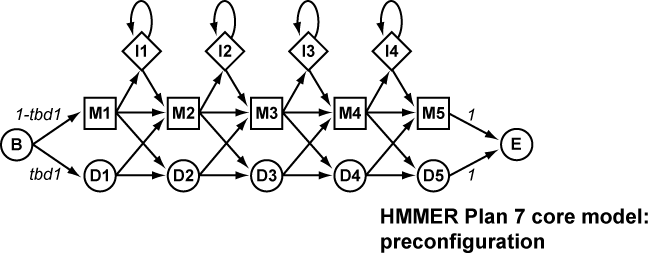
\includegraphics{plan7-core}
\caption{\textit{The core of the Plan7 architecture. Squares indicate
match states (modeling consensus positions in the alignment).
Diamonds indicate insert states (modeling insertions relative to
consensus) and special random sequence emitting states. Circles
indicate delete states (modeling deletions relative to consensus) and
special begin/end states. Arrows indicate state transitions. Every
match state and insert state also carries an emission probability
distribution, for the observable symbols (4 nucleotides or 20 amino
acids).}}
\end{figure}

A profile HMM is capable of modeling gapped alignments, e.g. including
insertions and deletions, which lets the software describe a complete
conserved domain (rather than just a small ungapped motif). Insertions
and deletions are modeled using (surprise!) insertion (I) states and
deletion (D) states. Each match state has an I and a D state
associated with it. HMMER calls a group of three states (M/D/I) at the
same consensus position in the alignment a ``node''.

These states are interconnected with arrows called \emph{state
transition probabilities}. The transitions are arranged so that at
each node, either the M state is used (and a residue is aligned and
scored) or the D state is used (and no residue is aligned, resulting
in a deletion-gap character, '-'). Insertions occur between nodes, and
I states have a self-transition, allowing one or more inserted
residues to occur between consensus columns. The transition to an I
state for the first inserted residue, followed by zero or more I
$\rightarrow$I self-transitions for each subsequent inserted residue,
is the probabilistic equivalent of the familiar gap-open and
gap-extend \emph{affine gap} penalty system, where one pays a
(usually) high cost for opening a gap and a (usually) lower cost for
extending it.

The model begins and ends with dummy non-emitting states, B and E.

This core section of the Plan 7 model, composed of M, D, and I nodes,
flanked by B and E states, is essentially a Krogh/Haussler profile
HMM.  This is the ``core model''. The core model controls the
\textit{data dependent} features of the model. All the probability
parameters in the main model are generally estimated from observed
frequencies of residues and transitions in a multiple sequence
alignment.

Unlike the original Krogh/Haussler and HMMER model architecture, Plan
7 has no D $\rightarrow$ I or I $\rightarrow$ D transitions. This
reduction from 9 to 7 transitions per node in the main model is one of
the origins of the name Plan 7. (The original Krogh/Haussler
architecture is called Plan 9 in parts of the HMMER source
code.)\footnote{The true origin of the codename is left undocumented,
as it reveals an inordinate fondness for bad science fiction
movies. Frighteningly, David Haussler understood immediately.}

\begin{figure}[t]
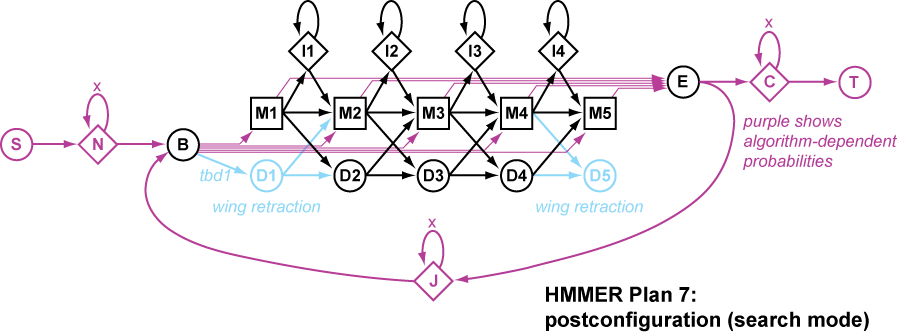
\includegraphics{plan7-search}
\caption{\textit{A complete Plan7 model, after configuration.}}
\end{figure}

The core model is augmented by five special states (S,N,C,T,J) and
additional state transition parameters to create the fully configured
Plan7 model. These additional states and parameters control
\textit{algorithm dependent} features of the model: e.g. how likely
the model is to generate various sorts of local or multihit
alignments. The algorithm dependent parameters are typically not
learned from data, but rather set externally by choosing a desired
alignment style.

In summary, the abbreviations for the states are as follows:

\begin{wideitem}
\item [\textbf{M$_x$}] Match state $x$.  Has $K$ emission probabilities.
\item [\textbf{D$_x$}] Delete state $x$. Non-emitter.
\item [\textbf{I$_x$}] Insert state $x$. Has $K$ emission probabilities.
\item [\textbf{S}]     Start state. Non-emitter.
\item [\textbf{N}]     N-terminal unaligned sequence state. 
    Emits \textit{on transition} with $K$ emission probabilities.
\item [\textbf{B}]     Begin state (for entering main model). Non-emitter.
\item [\textbf{E}]     End state (for exiting main model). Non-emitter.
\item [\textbf{C}]     C-terminal unaligned sequence state.
    Emits \textit{on transition} with $K$ emission probabilities.
\item [\textbf{J}]     Joining segment unaligned sequence state.
    Emits \textit{on transition} with $K$ emission probabilities.
\end{wideitem}

\subsubsection{the philosophy of Plan 7}

HMMs are \emph{generative probabilistic models}. Generative models
address a serious theoretical problem. To do correct statistical
inference, we need to be able to calculate a probability distribution
$P(S | M)$ for the probability of sequences $S$ given a model $M$, and
have this quantity sum to one over the ``space'' of all sequences.
But the number of possible different sequences $S$ is effectively
infinite, because they can be of any length. We can't just enumerate
this distribution, or we'd have to estimate an infinite number of
parameters. How do we make a \emph{finite} model of an \emph{infinite}
data space?  Generative models work by \emph{recursive} enumeration of
possible sequences from a finite set of rules -- rules that in an HMM
are represented by states, state transitions, and symbol emission
probabilities.

(In a profile HMM, the recursion is trivial: the self-transition
probability of the insert states, which allows insertions of any
length between two positions in the consensus. This simple model
implies a geometric distribution over insertion lengths -- as does any
linear or affine gap scoring system, in fact. Biologically, insertions
empirically follow a distribution with a longer tail, but more
realistic insertion models are computationally more expensive. The
marginal expected gain in performance is not thought to be worth the
extra computational effort.)

As described in \citep{Krogh94}, profile HMMs were originally
described as models of \emph{global alignment}: the sequence $S$ that
the model generates usually starts at the first match state and ends
at the last match state.

In real alignments of real biological sequences, global alignment is
rarely useful. A profile HMM is usually a model of a conserved domain,
not necessarily a model of a complete target sequence. A conserved
domain may be buried in a longer target sequence; there might be more
than one conserved domain in the target sequence; and maybe the target
sequence only contains a smaller fragment of the conserved domain. In
real applications, we prefer \emph{local alignment} algorithms, which
look for a high-scoring alignment between a subsequence of the target
sequence and a part of the query model. The common tools of sequence
analysis -- BLAST, FASTA, and Smith/Waterman alignment -- are all
local alignment algorithms.

It is straightforward to hack local alignment style algorithms around
the core Krogh/Haussler model of global alignment to a domain.  This
is what early versions of profile HMM software did, including
HMMER1. But some of the power of probabilistic modeling gets thrown
away; the resulting local alignment scores are no longer interpretable
as probabilities, because we have to introduce arbitrary
nonprobabilistic parameters for the local alignment (such as the usual
score of 0 for starting or ending a Smith/Waterman local alignment).

At least from a probabilistically purist perspective, it would be
sensible to revise the original Krogh/Haussler model to generate
\emph{complete} target sequences -- that is, modeling one or more
(possibly incomplete) matches to the domain model, and also modeling
the \emph{unaligned} sequence in the target. This is what Plan 7 does.

\subsubsection{the fully probabilistic ``local'' alignment models of Plan 7}

The Plan 7 architecture explicitly models the \emph{entire} target
sequence, regardless of how much of that sequence matches the main
model. \emph{All alignments to a Plan 7 model are ``global''
alignments:} a complete target sequence is aligned to a complete path
through the model from a start state (S) to the terminal state (T).
However, some (possibly most) of the sequence may be assigned to Plan
7 states (N,C,J) that generate nonhomologous, unaligned, ``random''
sequence that is not aligned to the main model.  Thus, the algorithm
dependent parts of the model control the \emph{apparent} locality of
the alignments.

Local alignments with respect to the sequence (i.e., allowing a match
to the main model anywhere internal to a longer sequence) are
controlled by the N and C states. If the N $\rightarrow$ N transition
is set to 0, alignments are constrained to have no unaligned
N-terminal sequence. Similarly, if the C $\rightarrow$ C transition is
set to 0, alignments are constrained to have no unaligned C-terminal
sequence.

Local alignments with respect to the model (i.e., allowing fragments
of the model to match the sequence) are controlled by B $\rightarrow$
M ``entry'' transitions and M $\rightarrow$ E ``exit'' transitions,
shown as dotted lines in the Plan 7 figure. Setting all entries but
the B $\rightarrow$ M$_1$ transition to 0 forces a partially
``global'' alignment in which all alignments to the main model must
start at the first match or delete state. Setting all exits to 0 but
the final M $\rightarrow$ E transition (which is always 1.0) forces a
partially global alignment in which all alignments to the main model
must end at the final match or delete state.

Multiple hit alignments are controlled by the E $\rightarrow$ J
transition and the J state. If the E $\rightarrow$ J transition is set
to 0, a sequence may only contain one domain (one alignment to the
main model). If it is nonzero, more than one domain per sequence can
be aligned to the main model. The J $\rightarrow$ J transition
controls the expected length of the intervening sequence between
domains; the lower this probability, the more clustered the domains
are expected to be.

\subsubsection{available alignment modes}

Because the alignment mode in Plan 7 is determined by the HMM
configuration, not by the search algorithm, you choose your alignment
style when you build the model -- not when you do the search.

The \prog{hmmbuild} program currently allows you to choose one of four
alignment modes, as follows. They are called \prog{hmmls},
\prog{hmmfs}, \prog{hmmsw}, and \prog{hmms} mode for historical
reasons -- these were the names of the corresponding search programs
in HMMER1.

\begin{wideitem}
\item [\emprog{hmmls}] This is like ``profile'' alignment or
``glocal'' alignment (as Waterman and others call it): global with
respect to the profile, and local with respect to sequence.  Multiple
nonoverlapping domains are allowed in the target sequence. $t_{NN}$
and $t_{CC}$ set to $t_{GG}$ from the null model (see below). $t_{EJ}$
set to 0.5. Internal entries and exits set to zero. This is the
default mode for HMMER.

\item [\emprog{hmmfs}] Multihit Smith/Waterman alignment: fully local
with respect to both the main model and the sequence; in addition,
multiple nonoverlapping alignments to more than one domain in the same
target sequence are allowed.  $t_{NN}$ and $t_{CC}$ set to $t_{GG}$
from the null model.  $t_{EJ}$ is set to 0.5.  Entry and exit
probabilities are set in a way such that all subsequences $i,j$ of the
model (starting at position $i$ and ending from position $j$) are
equiprobable (this is only roughly correct, as worded here; see source
code for detail). Activated by the \prog{hmmbuild -f} option.

\item [\emprog{hmmsw}] Smith/Waterman ``classic'' local alignment,
single best alignment per target. Same as \emprog{hmmfs} above, but
$t_{EJ}$ is set to zero. Activated by the \prog{hmmbuild -s} option.

\item [\emprog{hmms}] Needleman/Wunsch ``classic'' global alignment,
single best alignment per target. $t_{NN}$ and $t_{CC}$ set to
$t_{GG}$ from the null model. $t_{EJ}$ set to zero. Internal entries
and exits set to zero.  Activated by the \prog{hmmbuild -g} option.
\end{wideitem}

One advantage of Plan 7 is great flexibility in choosing an alignment
style. Complicated alignment styles are easily encoded in the model
parameters without changing the alignment algorithm.  For example, say
you wanted to model human L1 retrotransposon elements. Because of the
way L1 elements are inserted by reverse transcriptase (RVT), L1
elements tend to have a defined 3' end (RVT starts replication at the
same place in each new L1) but a ragged 5' end (RVT prematurely falls
off a new L1 in an unpredictable fashion). A specialized L1 model
could define non-zero internal entry probabilities and zero internal
exit probabilities to model this biological situation.

\begin{srefaq}{Why does Pfam distribute two sets of models, called
\prog{Pfam\_ls} and \prog{Pfam\_fs}?}  A disadvantage of Plan 7 is that
if you decide you want to do both local and global alignments, you
need two different models.  This wouldn't be too terrible, except for
the fact that the algorithm-dependent parameters strongly affect the
values of the $\mu$ and $\lambda$ parameters that E-value statistics
depend on. If the algorithm dependent parameters are changed, these
parameters are invalidated and the model needs to be recalibrated with
\prog{hmmcalibrate} -- but \prog{hmmcalibrate} is slow, so this can't
be done ``on the fly'' inside one of the search programs. It turns out
that ls mode is the most sensitive alignment mode, so long as a
complete domain alignment can be found; whereas fs mode is needed to
find domain fragments. Therefore Pfam is distributed with both sets of
models; for maximum detection ability of all homologies, both sets of
models have to be used.
\end{srefaq}

\subsection{Technical details on Plan 7 model configuration}

Skip this section unless you're interested in source code level detail.

In the figure of the fully configured Plan 7 architecture, you may
have noticed that the first and last delete states are greyed
out. Internally in HMMER, these delete states exist in the
``probability form'' of the model (when the model is being worked with
in every way except alignments) but they are carefully removed in the
``search form'' of the model (when the model is converted to log-odds
scores and used for alignments). This process is called ``wing
retraction'' in the code, by analogy to a swept-wing fighter changing
from a wings-out takeoff and landing configuration to a wings-back
configuration for high speed flight.

The technical problem that this is addressing is that the Plan 7 model
allows cycles through the J state. If a continuous nonemitting ``mute
cycle'' were allowed (J, B, D states, E, and back to J), dynamic
programming recursions would fail. This is why special mute states
like delete states must be handled carefully in HMM dynamic
programming algorithms \citep{Durbin98}. The easiest way to prevent a
mute cycle is to disallow them: make sure that the model must pass
through at least one match state per path through the main model.
Usually this can be done by breaking the chain somewhere and absorbing
the offending probability into a non-mute path.

Wing retraction involves folding the probabilities of the terminal
delete paths into the Plan 7 entry and exit probabilities. For
example, in wing retraction the ``algorithm dependent'' B
$\rightarrow$ M$_{3}$ entry probability is incremented by the
probability of the ``data dependent'' path B $\rightarrow$ D$_1$
$\rightarrow$ D$_2$ $\rightarrow$ M$_3$.

Wing retraction is done by the algorithm configuration routines. It is
only done for algorithms that allow beginning in or ending from a
delete state (global and glocal alignment modes). It is not done for
fully local Smith/Waterman modes (hmmfs and hmmsw modes) where the
algorithm-dependent begin and end distributions force entry and exit
only at match states.  Having the wing retraction step, rather than
{\em always} folding these probabilities together, is a design
decision, preserving a distinction between the ``algorithm dependent''
and ``data dependent'' parts of the model.

Because of wing retraction, the $D_1$ and $D_M$ states are never
accessed in dynamic programming alignment code. Their probabilities
are still kept in the model, so that the core model is remembered, and
a model can be ``deconfigured'' or reconfigured to a new algorithm
style. 

This leads to a peculiar technicality: the match state exit
transitions in a configured model can appear to be unnormalized,
because the exit transition from match state $k$ includes a dollop of
extra probability for the path that goes all-delete for the remainder
of the model ($k+1..M$). This is as should be, and everything balances
out, because exactly the sum of all those extra dollops of probability
get ignored when the DP algorithms ignore the final delete state.

\subsection{Parsing the residue information in input multiple sequence alignments}

\subsubsection{alphabet type: DNA or protein}

By default, the alphabet type (DNA or protein) is determined
automatically from the sequences in the alignment. This determination
primarily relies on the fact that some amino acid residues
(``EFIPQZ'') do not occur in DNA sequences, even in the IUPAC
degenerate code. Rarely, on small alignments, the autodetection may
resort to guesswork (and print a warning), or may fail altogether. You
can explicitly force the alphabet type using the \prog{--amino} or
\prog{--nucleic} option. 

\begin{srefaq}{Can HMMER make models of sequences other than DNA or
protein?} By default, HMMER requires DNA (RNA) or protein sequences.
But if you're willing to hack the code, the alphabet is configurable;
see the notes on the \prog{config.h} file,
page~\pageref{section:alphabet-config} in the installation section.
\end{srefaq}

\subsubsection{case insensitivity}

HMMER reads sequence residues in its input files in a
\emph{case-insensitive} manner.  (Internally, residues are handled
digitally, rather than alphabetically.) Other aspects of the file,
such as sequence names, preserve their case.

\begin{srefaq}{Why doesn't HMMER recognize Santa Cruz's SAM A2M format
properly?} HMMER can read an aligned FASTA format that is close, but
crucially not quite the Santa Cruz a2m format.  The real Santa Cruz
a2m format, used by the SAM profile HMM package, encodes match versus
insert column information in an upper vs. lower case convention in its
input files, and a - versus . convention for its gap characters.
Since HMMER digitizes residues case-insensitively, and treats
all gap characters identically in input files, this
information is lost. HMMER cannot currently read SAM a2m files
directly - even though the aligned fasta format is sometimes
called a2m! This is a historical misunderstanding of mine
about what the Santa Cruz format was; I thought it was simple...
\end{srefaq}

\subsubsection{handling of degenerate residue codes}

For amino acid sequences, HMMER accepts the standard IUPAC degeneracy
codes (BZX). It reads U (selenocysteine) as a valid amino acid, and
treats it as a serine (S). (Selenocysteine is derived from serine in
vivo, so this seems as good a choice as any.) It does not accept the
IUPAC \prog{*} character for stop codons.

For nucleic acid sequences, it accepts the standard IUPAC degeneracy
codes (NRYMKSWHBVD). It treats U and T as the same residue, and thus
does not distinguish in any way between RNA and DNA.  It treats X as
if it were N, to humor the many bioinformatics software packages that
aren't IUPAC-compliant.

It handles degenerate codes probabilistically, by assuming a uniform
distribution over the possible residues. That is, an amino acid of X
counts as a probability $\frac{1}{20}$ for each of the 20 residues.


\subsection{Model architecture construction}

Not all of the columns of the multiple alignment will necessarily be
treated as consensus (match) columns. Some may be treated as
insertions relative to the consensus. Only the consensus columns will
get a model node (a trio of M/D/I states) assigned to them.  The
assignment of alignment columns as either ``consensus'' or ``insert''
is called \emph{model architecture construction}. HMMER allows
a choice of three architecture construction algorithms.

\subsubsection{maximum a posteriori model architecture construction, the default}

By default, HMMER uses a maximum a posteriori (MAP) architecture
algorithm, e.g. one that is guaranteed to find the model architecture
with the highest posterior probability for the alignment data
\citep{Durbin98}.  This is a dynamic programming algorithm, and it is
almost always fast enough that you won't notice that it's running --
the rate limiting step in model construction is more often the
sequence weighting algorithm (see below). 

The MAP algorithm incorporates a prior distribution over expected
model size. The prior holds the model sizes down and has the effect of
requiring a certain amount of information content per column before it
becomes worthwhile to make it a consensus column. This prior is a
geometric distribution, controlled by a single parameter which can be
set by the \prog{--archpri <x>} option to any number $0 \leq x \leq
1$. By default, it is set to 0.85. Increasing it favors longer models;
decreasing it favors shorter models. The default setting was
determined empirically, and should be considered to be an \emph{ad
hoc} parameter, since it implies a mean expected model length of only
7 consensus residues and is unrelated to the observed distribution of
protein domain consensus lengths.

\begin{srefaq}{Why did hmmbuild build a model of length 0 for my alignment?}
It is rare but possible for the MAP architecture algorithm to decide
that the optimal architecture is \emph{nothing} -- e.g. that there is
so little information in the alignment, it isn't even worth modeling
it as a consensus, because the null model is a better model of
it. This can happen if your alignment contains unrelated sequences, or
if it has a lot of sequence fragments (and hence a lot of gaps). You
should probably take this as a warning that your alignment may not be
very good. If you want to work around the effect, either increase the
architecture prior parameter using the \prog{--archpri} option, or use
one of the other two architecture construction algorithms,
\prog{--fast} or \prog{--hand}.
\end{srefaq}

\subsubsection{fast model architecture construction}

The \prog{--fast} option selects an alternative, heuristic model
architecture algorithm: all columns that contain more than a certain
fraction $x$ of gap characters will be assigned as an insert column.
This is the original Krogh/Haussler method \citep{Krogh94}.

By default, $x$ is 0.5. It can be set to something else using the
\prog{--gapmax <x>} option. $x$ can be anything between 0 and 1.  The
larger $x$ is, the more columns will be included in the consensus; at
$x=1$, all columns will be included, and at $x=0$, only columns that
contain all aligned residues (e.g. no gaps at all) will be called
consensus columns.

\subsubsection{hand model architecture construction}

If the input alignment is in annotated Stockholm (or SELEX) format, it
can have an RF (reference) coordinate line. The \prog{--hand} option
tells \prog{hmmbuild} to parse the RF line, and use it to determine
the architecture. Any column marked with a non-gap character (x, for
instance) in the RF line is assigned as a consensus column; any column
marked with a gap character in the RF line is assigned as an insertion
column.

Hand construction can come in, well, handy. For example, one can pick
a ``canonical'' sequence in the alignment, copy that aligned sequence
as the RF annotation, and a hand-built model will then have its model
nodes numbered exactly in the coordinate system of the canonical
sequence. (I do this for some families where I know one sequence so
well, I remember some of its residues by number, and I want the HMM to
number aligned residues the way I expect.)

HMMER propagates an appropriate RF annotation line into every new
multiple alignment it builds with \prog{hmmalign}. If you build a new
model from that new alignment, \prog{hmmbuild --hand} causes the new
model to have the same consensus architecture as the first model
(e.g. the model that made the alignment) -- for instance, the column
that was aligned to match state 43 in the first model gets assigned to
match state 43 in the new model. This provides a way to maintain a
fixed model architecture through iterations of
\prog{hmmbuild}/\prog{hmmsearch}/\prog{hmmalign}, even as the number
of sequences changes.

If you select \prog{--hand} but an RF annotation line is not present
on the alignment, \prog{hmmbuild} will fail with an error message, of
course.

\subsection{Collecting observed emission/transition counts}

Having assigned all the columns as consensus columns or insertion
columns, \prog{hmmbuild} now collects counts of symbol emissions
(residues) and state transitions (insertions/deletions) from the
alignment. The raw counts are adjusted by a few heuristics as follows.

\subsubsection{sequence weighting}

A profile HMM has no notion of phylogeny. It assumes, in fact, that
all the observed sequences are independent, uncorrelated samples from
a single model. This is clearly not true in any biological sequence
data set, because sequences are related to each other by speciation
and gene duplication events on a phylogenetic tree -- not to mention
trivial redundancy in the sequence databases. Therefore, HMMER applies
a sequence weighting algorithm to downweight counts from closely
related sequences, and upweight distantly related sequences.

The default weighting algorithm is the Gerstein/Sonnhammer/Chothia
tree weighting algorithm \citep{Gerstein94}. 

Several weighting schemes are available as options, as follows:

\begin{tabular}{lll}
Option            & Weighting method   &  Reference \\ \hline
\prog{--wblosum}  & Henikoff simple filter weights  & \citep{Henikoff92} \\
\prog{--wgsc}     & GSC tree weights (default)      & \citep{Gerstein94}\\
\prog{--wme}      & maximum entropy (ME)            & \citep{KroghMitchison95}\\
\prog{--wpb}      & Henikoff position-based weights & \citep{Henikoff94b}\\
\prog{--wvoronoi} & Sibbald/Argos Voronoi weights   & \citep{Sibbald90}\\
\prog{--wnone}    & don't do any weighting          & \\ \hline
\end{tabular}

Most of the available weighting algorithms will become rather slow for
large numbers of sequences (scaling with the square of the number of
sequences). If you are trying to weight by the GSC, BLOSUM, or Voronoi
methods, for alignments over a threshold of $n$ sequences, the
weighting algorithm is instead switched automatically to the
\prog{--wpb} style, Henikoff position based weights
\citep{Henikoff94b}. The default switching threshold is 1000 sequences;
this can be adjusted with the \prog{--pbswitch <n>} option. Set
\prog{--pbswitch} to something very large if you don't want this
algorithm switching behavior to happen.

The \prog{--wblosum} scheme works by single linkage clustering of all
sequences related by more than some threshold $x$ of fractional
sequence identity, then distributing a weight of 1 across each
cluster. By default $x$ is 0.62 (62\%), the rule used for weighting
the BLOSUM62 scoring matrix \citep{Henikoff92}. The \prog{--idlevel
<x>} option can be used to set the threshold to something else.
Beware, \prog{--idlevel} also affects the effective sequence number
calculation, as described in the next subsection.

There is no satisfactory theory behind setting the weights; this is an
\emph{ad hoc} step. The maximum entropy method comes with the most
theoretical motivation, but even it is a bit of a stretch as far as
biological realism. A correct model would incorporate an explicit
model of phylogeny (e.g. ``tree HMMs'' \citep{Mitchison95}). There is a
growing body of literature from Jotun Hein, Ian Holmes, Bill Bruno,
Richard Goldstein and others, moving towards combining profile HMMs
and explicit phylogenetic modeling.

\subsubsection{determining the effective sequence number}

For $N$ sequences, sequence weighting algorithms typically
redistribute a total of $N$ counts, such that some sequences get
weights less than 1, some have weights larger than 1, but overall each
sequence has an average weight of 1. In principle, though, the total
sequence weight could be an arbitrary number, not necessarily $N$;
here, call it $X$, the \emph{effective sequence number}. 

For example, if our alignment contained 20 sequences, but 10 of them
were identical copies of the same sequence due to trivial database
redundancy, we'd not only want to downweight those sequences so that
they counted 1/10 as much as the other ones; we'd want to treat the
alignment as a total of 11 sequences, not 20.

Normally, sequence weighting algorithms ignore this issue because it
cancels out: if we were going to estimate probability parameters as
simple frequencies (e.g. maximum likelihood parameter estimation), the
choice of $X$ is irrelevant.

Profile HMMs do not estimate probability parameters solely from
counts, though. Observed count data are combined with \emph{priors},
which incorporate \emph{a priori} knowledge about what homologous,
aligned sequences usually look like; profile HMM parameters are
\emph{mean posterior estimates}, not maximum likelihood estimates
\citep{Durbin98,Sjolander96}. The less count data there are, the more
the priors affect the parameter estimates, so the choice of effective
sequence number $X$ becomes relevant.

HMMER determines effective sequence number by the BLOSUM clustering
rule: it counts the number of single linkage clusters above some
threshold fractional identity $x$, where $x$ defaults to 0.62.  The
threshold can be changed with the \prog{--idlevel <x>} option (beware,
that changes the behavior of the rarely used \prog{--wblosum}
weighting option too). Note that $X \leq N$. At \prog{--idlevel 0},
all sequences are clustered into one group, and $X=1$; at
\prog{--idlevel 1}, no sequences are clustered, and $X=N$.

The effective sequence number calculation can be shut off using the
\prog{--noeff} option.

There is no satisfactory theory behind the \emph{ad hoc}-ery of the
effective sequence number. Explicit phylogenetic methods will someday
make it obsolete.

\subsubsection{adjustments to the alignment}

Don't be shocked, but if you used a \prog{--hand} or \prog{--fast}
architecture construction strategy, the alignment that HMMER builds
its model from is not necessarily exactly the alignment that you
provided.

The reason is that the Plan 7 design disallows D $\rightarrow$ I and I
$\rightarrow$ D transitions, but your alignment may imply them.  For
instance, consider a hand-built model from this alignment:

\begin{sreoutput}
#=GC RF   xx..xx
seq1      C-a.YH
seq2      CM.v-H
\end{sreoutput}

seq1 implies a D$_2$ $\rightarrow$ I$_2$ transition, and seq2 implies
an I$_2$ $\rightarrow$ D$_3$ transition. These illegal moves have to
be dealt with somehow, before a valid Plan7 model can be built. HMMER
does something truly ugly to get around this - an evil little routine,
\prog{modelmaker.c:trace\_doctor()}, quietly \emph{revises} the
alignment to make it compatible with Plan 7.  D $\rightarrow$ I moves
are fixed by shoving the insertion to the left, filling the deletion
and turning it into a match.  I $\rightarrow$ D moves are fixed by
shoving the insertion to the right. There are a few other types of
illegal moves at the beginning and end of the model that
\prog{trace\_doctor()} also deals with.

Fortunately this is rare. If you want to see what HMMER did to your
beautiful alignment, you can use the \prog{-o <alifile>} option to
output a copy of your alignment \emph{after} hmmbuild has worked its
evil magic on it - the match columns will be annotated with an RF
line, and some residues may have been realigned. For instance, a
resaved copy of the above example, after \prog{hmmbuild --hand -o},
is:

\begin{sreoutput}
# STOCKHOLM 1.0
#=GF AU    HMMER 2.2g

seq1        CAYH
seq2        CMVH
#=GC RF     xxxx
//
\end{sreoutput}

and the gaps have (not so mysteriously, now?) disappeared.

\subsection{Estimating probability parameters from counts}

Counts $c_x$ are converted to mean posterior probability estimates
$\hat{p}_x$ using mixture Dirichlet priors.  The equation is

\[
  \hat{p}_x = \sum_k P(k | \vec{c})
  \frac{c_x + \alpha_x^k}{\sum_{y} (c_y + \alpha_{y}^k) }
\]

for a mixture of Dirichlet parameters $\alpha$, with each individual
Dirichlet mixture component numbered by $k$. The probability of
mixture $k$ given the count vector $\vec{c}$, $P(k | \vec{c})$, is a
mess of gamma functions; its equation is given by Sj\"{o}lander
\citep{Sjolander96,Durbin98}.

In the case of a single-component Dirichlet, this equation reduces to:

\[ 
  \hat{p}_x = \frac{c_x + \alpha_x}{\sum_{y} (c_y + \alpha_{y}) }
\]

where the $\alpha$ terms are often thought of as \emph{pseudocounts},
because they are added to the count data as if they were observations.
The bigger the alpha terms, the more weight the prior has, and the
more count data it takes to override the prior.

Each emission and transition probability distribution in the
data-dependent parts of a Plan 7 model have a prior assigned to them.
HMMER has hardcoded defaults; copies of these defaults are in
\prog{tutorial/amino.pri} and \prog{tutorial/nucleic.pri}, in HMMER's
prior file format (see page~\pageref{section:priorfiles}).

For proteins, the match emission prior is the nine-component Blocks9
mixture from Sj\"{o}lander et al. \citep{Sjolander96}. The insert
emission prior is a slightly hydrophilic-biased distribution estimated
from inserted residues in an early version of the Pfam database. The
insert prior has then been artificially scaled to very high values of
$\alpha$, which has the effect of fixating the insert emission
distributions in HMMER: all insertion states have virtually identical
emission distributions, rather than learning from the observed data.
The transition priors for M, D, and I states are single-component
Dirichlets, estimated by maximum likelihood on an early version of
Pfam by Graeme Mitchison.

No attempt has been made to estimate good nucleic acid priors.  The
transition priors are copied from the protein set. The match and
insert emission priors are \emph{plus-one} (Laplace) priors.

\subsubsection{using customized priors}

The default priors can be overridden on the command line, by providing
a prior file with the \prog{--prior <f>} option to \prog{hmmbuild}.

\subsubsection{the \emph{ad hoc} PAM prior}

An alternative to Dirichlet priors is available, called PAM priors,
which uses an amino acid scoring matrix to contribute prior
information.  It is activated by providing a scoring matrix file with
the \prog{--pam <f>} option. There is a weighting parameter $A$ that
affects how much weight (in counts) the prior has; by default $A=20$,
but this can be set with the \prog{--pamwgt <x>} option. This
implements the ``substitution matrix mixture'' strategy discussed by
Durbin et al. on p.117-119 \citep{Durbin98}.

\subsection{Calculating scores from counts}

The alignment scores reported by HMMER are log-odds scores: the log of
the probability of the sequence given the HMM, divided by the
probability of the sequence given a ``null hypothesis'' that the
sequence is just a random sequence, unrelated to the HMM
\citep{Barrett97}. The ``null model'' is also a probabilistic model,
but a simpler one than the profile:

\begin{center}

\includegraphics{nullmodel}
\end{center}

The G state has a symbol emission probability distribution for $K$
symbols in the alphabet. By default, this distribution is set either
to the average amino acid composition of SWISSPROT 34, or to 0.25 for
each nucleotide. The G $\rightarrow$ G transition controls the
expected length of observed random sequences; in practice, this
transition probability is so close to 1 that it has very little
effect. (It is set to 350/351 for protein models, 1000/1001 for DNA
models.) The F state is just a dummy end state like the T state in the
Plan 7 architecture.

The score of residues $x$ in match or insert states are:
\[
  s_x = \frac{p_x}{g_x}
\]

where $p_x$ is the probability according to the HMM, and $g_x$ is the
probabilitity according to the null model. Transition scores are also
calculated as log odds parameters. For details, see the source
documentation in \prog{plan7.c:P7Logoddsify()}.

As with the priors, copies of the default null model parameters are
provided, in the files \prog{tutorial/amino.null} and
\prog{tutorial/nucleic.null}.

Alternative null model files may be provided using the \prog{--null
<f>} option to \prog{hmmbuild}.

\subsection{Setting the alignment mode}

The model is then configured in one of four different alignment modes,
as described above. The default is hmmls mode: global with respect to
the model, multihit-local in the target sequence(s). The other modes
are selected with options:
\begin{enumerate}
\item[\prog{-f}] hmmfs, ``fragment'' mode: local in model,
multihit-local in sequence.
\item[\prog{-g}] hmms, ``global'' mode: global in model,
single hit global in sequence.
\item[\prog{-s}] hmmsw, ``Smith/Waterman'' mode: local in model,
single hit local in sequence.
\end{enumerate}

\subsection{Naming and saving the HMM}

HMM files have names (enabling them to be used in multi-HMM databases
for hmmpfam, like Pfam). The name must be one word, containing
no whitespace. The name is obtained in one of three ways:

\begin{itemize}
\item if a name \prog{<s>} is explicitly provided by the \prog{-n <s>}
      option, that's the name;
\item else if the alignment has a name (Stockholm \verb+#=GF ID+ or
      SELEX \verb+#=ID+ annotation), that's the name;
\item else the name is constructed by stripping off any suffix
      from the alignment file name. For instance, the alignment file
      ``rrm.phylip'' would result in an HMM named ``rrm''.
\end{itemize}
      
Finally, the HMM is saved. The default is to save it to the file named
on the \prog{hmmbuild} command line in a flat text, readable ASCII
format (page~\pageref{section:savefiles}. If the file already exists,
HMMER refuses to overwite it unless the \prog{-F} option was used to
force the overwrite, or the \prog{-A} option was used, which appends
to an existing HMM file rather than making a new HMM file.

A more space-efficient but undocumented binary format is available,
selected with the \prog{--binary} option. (Do not append binary HMMs
to ASCII files or vice versa; the program doesn't check to be sure
you're not doing this.) Minor but significant speed gains can be
obtained by working with large HMM databases in binary
format. Usually, one would convert an entire database to binary at
once, using the \prog{hmmconvert} program.





\newpage
\section{How HMMER scores alignments and determines significance}

The search programs \prog{hmmsearch} and \prog{hmmpfam} give you a
ranked list of hits in a sequence database.  Which ones are likely to
be true homologous and which ones are likely to be nonhomologous to
your query HMM?

HMMER gives you at least two scoring criteria to judge by: the HMMER
raw score, and an E-value. Additionally, Pfam models carry a third set
of criteria: six expert-calibrated raw score cutoffs that the Pfam
database maintainers set. How should you interpret all this
information?

\subsection{Executive summary}

\begin{itemize}
\item The best criterion of statistical significance is the E-value.
The E-value is calculated from the bit score. It tells you how many
false positives you would have expected to see at or above this bit
score. Therefore a low E-value is best; an E-value of 0.1, for
instance, means that there's only a 10\% chance that you would've seen
a hit this good in a search of nonhomologous sequences. {\em
Typically, I trust the results of HMMER searches at about E=0.1 and
below, and I examine the hits manually down to E=10 or so.}

\item HMMER bit scores are a stricter criterion: they reflect whether
the sequence is a better match to the profile model (positive score)
or to the null model of nonhomologous sequences (negative score).  A
HMMER bit score above $\log_2$ of the number of sequences in the
target database is likely to be a true homologue. For current NR
databases, this rule-of-thumb number is on the order of 20 bits.
Whereas the E-value measures how statistically significant the bit
score is, the bit score itself is telling you how well the sequence
matches your HMM. Because these things should be strongly correlated,
usually, true homologues will have both a good bit score and a good
E-value. However, sometimes (and these are the interesting cases), you
will find remote homologues which do not match the model well (and so
do not have good bit scores -- possibly even negative), but which
nonetheless have significant E-values, indicating that the bit score,
though ``bad'', is still better than you would've expected by chance,
so it is suggestive of homology.

\item For Pfam HMMs, you can also examine six other numbers that
represent bit score thresholds: two TC (trusted cutoff) scores, two GA
(gathering) scores, and two NC (noise cutoff) scores. The meaning of
these numbers is described below.
\end{itemize}

\begin{srefaq}{What does it mean when I have a negative bit score,
but a good E-value?} The negative bit score means that the sequence is
not a good match to the model. The good E-value means that it's still
a better score than you would've expected from a random sequence. The
usual interpretation is that the sequence is homologous to the
sequence family modeled by the HMM, but it's not ``within'' the family
- it's a distant homologue of some sort. This happens most often with
HMMs built from ``tight'' families of high sequence identity, aligned
to remote homologues outside the family. For example, an actin HMM
aligned to an actin-related protein will show this behavior - the bit
score says the sequence isn't an actin (correct) but the E-value says
it is significantly related to the actin family (also correct).
\end{srefaq}

\subsection{In more detail: HMMER bit scores}

The bit score is a log-odds score in log base two (thus, in units of
{\em bits}. Specifically, it is:

\[
	S = \log_2 \frac {P( \mbox{seq} | \mbox{HMM})} { P (\mbox{seq} |
	\mbox{null})}.
\]

$P( \mbox{seq} | \mbox{HMM})$ is the probability of the target
sequence according to your HMM. $ P (\mbox{seq} | \mbox{null}) $ is
the probability of the target sequence given a ``null hypothesis''
model of the statistics of random sequence. In HMMER, this null model
is a simple one-state HMM that says that random sequences are i.i.d.
sequences with a specific residue composition (this ``null model
distribution'' is part of the HMM save file, and it can be altered
when you do an \prog{hmmbuild}).

Thus, a positive score means the HMM is a better model of the target
sequence than the null model is (e.g. the HMM gives a higher
probability).

\prog{hmmsearch} reports two hit lists, with different types of
scores. The first list is ranked by {\em per-sequence} scores, and the
second is ranked by {\em per-domain} scores. The per-sequence score is
the score of the entire target sequence according to the HMM. A
per-domain score is a score of one matching subsequence (domain) from
the target sequence: the per-domain score is calculated as if that
subsequence was the entire target sequence.

Because HMMER's Plan 7 model is capable of looping, and therefore of
modeling more than one copy of a particular domain in a target
sequence (for instance, a closely spaced array of immunoglobulin
superfamily domains), HMMER may well report more than one domain per
target sequence.

For single domain proteins, the per-sequence and per-domain scores are
identical. For multi-domain proteins, the per-sequence score is the
sum of the individual per-domain scores.

You can specify cutoffs for per-sequence and/or per-domain scores
and/or E-values when you use \prog{hmmsearch} or \prog{hmmpfam}.  For
a specific sensible use of such cutoffs, read about how the Pfam
TC/NC/GA cutoffs are set and used (below).

\subsubsection{interaction of multihit alignment with negative bit scores}

HMMER will always report a score for the one best domain it finds in
the target sequence, even if that hit is a negative bit score.  The
Plan 7 model architecture forces a target sequence to pass through the
model at least one time.

However, each \emph{subsequent} domain must have a positive bit score
to be identified. If an additional domain has a negative bit score,
HMMER can find a better scoring alignment by using the
``nonhomologous'' N, C, or J states to account for the residues in
that domain -- \emph{even if the domain would have a significant
E-value}.

\begin{srefaq}{Why does HMMER give this domain a good E-value when
I just give it the domain sequence, but it doesn't find the domain at
all in the context of the whole sequence the domain came from?}  See
above. The behavior of being able to report the single best hit,
regardless of score, produces one counterintuitive behavior:
statistically significant domains will be invisible in a sequence if
they have negative bit scores. You can find cases where you can find
additional domains with good E-values but negative bit scores by
searching against a sequence that you've cut into smaller pieces. This
is not a bug; it's a limitation of the approach.
\end{srefaq}


\subsection{In more detail: HMMER E-values}

The E-value is the expected number of false positives with scores at
least as high as your hit.

Unlike the raw score, the E-value is dependent on the size of the
database you search. If you detect a hit with an E-value of 0.1 in a
search of a sequence database with 100,000 sequences, then you happen
to re-score the sequence all by itself, you will get an E-value
100,000 times better. The E-value is quite literally the expected
number of false positives at this raw score; the larger the database
you search, the greater the number of expected false positives.

\begin{srefaq}{Why do I get a different E-value when I search
against a file containing my sequence, than I got when I searched the
database?} See above. This behavior is shared with BLAST and FASTA
P-value and E-values, so it should not be unfamiliar to most users.
However, it can cause consternation: a related phenomenon is that a
hit that is marginally significant this year may no longer be
significant next year, when the database is twice as large. You can
specify a database size with the \prog{-Z} option.
\end{srefaq}

\begin{srefaq}{Why do hmmsearch and hmmpfam give me different
E-values?} From the above discussion, it should also be clear that if
you use \prog{hmmpfam} to search a sequence against Pfam (say, $\sim
3000$ models) to find a matching HMM, you will get a different E-value
than using \prog{hmmsearch} to search that single HMM against a
sequence database to find the original sequence, because the size of
the search spaces is entirely different. For hmmpfam, the search space
size $Z$ is the number of \emph{models}; for hmmsearch, the search
space size $Z$ is the number of \emph{sequences}. Some people want to
argue that this is wrong, but it's something you have to deal with;
that's statistics for you.
\end{srefaq}

HMMER has two ways of calculating E-values. One way is inaccurate but
analytical (and fast); the other way is more accurate but empirical
(and slow).

If your HMM has not been calibrated with \prog{hmmcalibrate}, HMMER
uses the analytic calculation. This is a conservative calculation,
meaning that the ``true'' E-value will be lower; sometimes much lower.
The calculation is essentially the same as that given in
\cite{Barrett97}.

It is highly recommended that you calibrate HMMs with
\prog{hmmcalibrate}. \prog{hmmcalibrate} writes two parameters
into your HMM file on a line labeled ``EVD'': these parameters are the
$\mu$ (location) and $\lambda$ (scale) parameters of an extreme value
distribution (EVD) that best fits a histogram of scores calculated on
randomly generated sequences of about the same length and residue
composition as SWISS-PROT. You only need to do this calibration once
for a given HMM. All the Pfam HMMs come pre-calibrated.

\subsubsection{fitting extreme value distributions to HMMER score histograms}

Now, there's good news and bad news about extreme value distributions.

Frst the good news. The extreme value distribution fitting is done
with a rather robust and personally satisfying chunk of maximum
likelihood code (see \prog{histogram.c} in the codebase). The ML
approach was suggested to me by Stephen Altschul, who directed me to a
lovely textbook by Lawless \cite{Lawless82}.  A brief technical report
on HMMER's EVD fitting is available at
\htmladdnormallink{ftp://ftp.genetics.wustl.edu/pub/eddy/papers/evd.pdf}
{ftp://ftp.genetics.wustl.edu/pub/eddy/papers/evd.pdf}.  Any EVD
fitting code that is relying on linear regression fits to log-log
plots is bound to be less accurate, judging from my tests.

However, the down side is that most profile HMM scores don't fit the
extreme value distribution well. Fully local alignments (models built
with \prog{hmmbuild -f} or \prog{hmmbuild -s} fit the EVD fairly well,
as expected for Smith/Waterman style alignments, for the same reasons
that gapped BLAST or FASTA alignment scores have been shown to be
approximately EVD-distributed. By default, though, \prog{hmmbuild}
makes models for ``glocal'' alignments which are global with respect
to the model, and multi-hit-local with respect to the sequence.  Also
called ``profile scores'' by Waterman, this sort of alignment score is
known not to be EVD-distributed \cite{GoldsteinWaterman94}.

Nonetheless, empirically, the tail of the distribution around E=1 is
falling off more or less like an EVD, and this is the region of
interest. HMMER does a ``censored EVD fit'' from the peak of the
distribution down to the right tail, and does not include the data to
the left of the peak in its fit. This produces a reasonable fit in the
important region of the scores. Empirically, HMMER E-values tend to be
accurate in the critical region (E~1), despite the lack of
mathematical foundation.

The end of \prog{hmmsearch} output shows you the observed histogram,
and (if the model is calibrated) an expected curve according to the
EVD fit. You should observe that the relevant tail (around E=1) is
more or less well fitted. The bulk of the distribution, particularly
at lower scores, is usually poorly fitted, but this is not the area of
interest.

\subsection{In more detail: Pfam TC/NC/GA cutoffs}

When a Pfam model is built, the Pfam curation team keeps track of
per-sequence and per-domain scores of every sequence in a large
nonredundant database. They record three types of score cutoffs on
Pfam HMM files:

\begin{wideitem}
\item[GA (gathering cutoffs)]: the scores used as cutoffs in
constructing Pfam. All domains that are in a sequence satisfying the
GA1 per-sequence score, and which themselves satisfy the GA2
per-domain score, will be included in the Pfam ``full alignment''.

\item[TC (trusted cutoffs)]: the scores of the lowest-scoring hit(s)
that were included as true member(s) of the Pfam family. The
per-domain TC2 score is the score of the lowest scoring domain
\textit{in a sequence with a per-sequence score over the TC1 cutoff};
therefore, the TC1 and TC2 scores could conceivably come from
different targets. Hits above these scores are ``within'' the Pfam
family and almost certainly members.

\item[NC (noise cutoffs)]: the scores of the highest-scoring
hit(s) that were \textit{not} included as true members of the Pfam
family, because they were considered to be the top of the noise.
Calculated analogously to TC1 and TC2. Hits above the NC cutoff are
above the top scoring noise in the Pfam NR database search, so are
likely homologues, but not as trustworthy as hits over the GA or TC
cutoffs.
\end{wideitem}

In order of increasing conservativeness, the cutoffs rank: NC, GA, and
TC.

The GA cutoffs, being the actual cutoffs used in constructing Pfam,
are a very good choice to use to collate large-scale automated data,
like counting protein family members in a sequenced genome.

The TC and NC cutoffs are less useful, and only really there as
documentation of Pfam construction. In general, the TC cutoffs would
be extremely conservative cutoffs to use in a database search, more
conservative than GA. The NC cutoffs are less conservative than GA.

Why use GA (or the other cutoffs) instead of the E-value? Pfam
artificially imposes a ``flat'', nonhierarchical structure on protein
sequence space.  Pfam asserts that no Pfam family is related to any
other Pfam family. This is obvious nonsense: many Pfam families are in
fact homologous.  The different 7-TM (G-protein coupled receptor)
families are one example; the different GTPase families are
another. HMMER often detect significant relationships between families
that Pfam chooses to suppress. In these cases, the Pfam GA cutoff will
be elevated to artifically separate two homologous but distantly
related subgroups of the same structural superfamily. 

\begin{srefaq}{Why isn't sequence X included in a Pfam full alignment?
It has a significant score!} For the reasons above, the sequences in
Pfam full alignments are harvested using curated GA
thresholds, rather than using score or E-value
thresholds. Interpro-based counts of domains in genome analyses also
use curated GA thresholds.  Please don't go writing a
paper that claims HMMs don't detect some similarity until you've done
the experiment with HMMs instead of just looking at curated Pfam
classifications. Yes, such paper(s) have been written. Sigh.
\end{srefaq}

The mechanism that HMMER uses to incorporate up these cutoffs is
general: Stockholm format multiple sequence alignments can carry
appropriate TC, NC, and GA markup lines. This means that you can use a
Pfam-like cutoff system if you like, just by adding the appropriate
Stockholm markup to your collection of alignments. When these numbers
are available in the HMM, HMMER search programs provide options
(\prog{--cut\_ga}, etc.) for setting search cutoffs to GA, TC, or NC
automatically.

\subsection{Biased composition filtering: the null2 model}

I've lied. HMMER bit scores are actually calculated as log odds scores
relative to \emph{two} null hypotheses. The first is the null model
built into the profile HMM when it was built with \prog{hmmbuild}.
The second, called \emph{null2}, is an \emph{ad hoc} model calculated
on the fly for each alignment, from the characteristics of that
alignment. The purpose of null2 is to compensate for false positive
hits caused by simple biased composition regions in the target
sequence.

Common biased composition filters like XNU, DUST, and SEG are
qualitative filters -- if a region is detected as biased composition,
it is masked (the residues are converted to X's). A drawback of this
approach is that some real domains are biased composition --
collagens, for example, are almost completely masked by standard
filters, and you won't see true collagen homologies.  The HMMER
composition filter is a quantitative filter, that tests whether the
sequence is a better match to the profile HMM, the null (random
composition) model, or a null2 model of biased amino acid composition.

This is a Good Thing, but on the other hand, the null2 model is not
very sophisticated. It is a single-state HMM just like the main null
model, which means it only captures residue composition, like DUST; no
attempt is made in HMMER to filter short-period repetitive sequences
like the XNU algorithm does. (The XNU masking algorithm is available
as an option, \prog{--xnu}.)

The null2 model was motivated by an artifact that appeared in the Plan
7 implementation of HMMER2. In HMMER1, insertion emissions always
scored zero: the insertion emission distribution was assumed to be
identical to overall amino acid composition. But that loses a small
amount of information. On average, insertions tend to occur in surface
loops of proteins. Inserted residues have a small but significant
hydrophilic bias. HMMER2's parameterization takes that into account.
As a result, insertions of hydrophilic residues get slightly positive
scores, while insertions of hydrophobic residues get slightly negative
scores.

\begin{srefaq}{Why is my alignment annotating inserted residues with
+'s? Shouldn't +'s only appear for aligned consensus residues?} This
is not a bug. See above; certain inserted residues can contribute
positive score to the alignment, because they are slighly more likely
to be seen in insertions than in overall amino acid composition.
\end{srefaq}

If you give hydrophilic insertions positive score, and you combine
that with the ability to do Smith/Waterman local alignment, you get an
undesirable artifact: it's possible to get alignments that enter the
model at some match state, align a residue to that match state, then
proceed to use the insertion state for a long hydrophilic stretch
before exiting the model from the next match state: thus, a ``high
scoring'' alignment that aligns to only two consensus positions in the
model, with a long insertion. It's this artifact that motivated the
development of the null2 filter, though the null2 filter also happens
to work well on a variety of other biased-composition scenarios.

A different null2 model is calculated for every alignment. The 20
emission probabilities of the null2 model are calculated as the
occurrence-weighted average emission probability of all the states in
the alignment's state path $\pi$. For example, if the state path is 52
emissions long and contains M$_{32}$, 50 inserted residues aligned to
I$_{32}$, and M$_{33}$, the null2 model will be calculated by averaging 52
emission distributions (50 copies of I$_{32}$, 1 each of M$_{32}$ and
M$_{33}$). 

But now we've got \emph{two} null hypotheses. We said we report a bit
score that's a log-odds ratio of our model likelihood and \emph{one}
null hypothesis likelihood. How do we calculate a score if we have
more than one null hypothesis? HMMER does a bit of algebraic sleight
of hand here, to arrive at an additive correction to the original
score that it calls the ``null2 score correction''. 

Because the mysterious null2 correction generated a fair amount of
faq-ish email traffic in the past, let's now finally slog through and
document the null2 score correction calculation, and the unpublished
(but relatively trivial) theory behind it.

\subsubsection{derivation of the null2 score correction}

We arrived at the parameters of the null2 model in a very \emph{ad
hoc} way. However, after that, the way HMMER arrives at the final bit
score once the null2 parameters have been determined is clean
(e.g. derivable) Bayesian probability theory, and sort of a novel
idea for quantitative sequence masking, I think.

If we take the Bayesian view, we're interested in the probability of a
hypothesis $H$ given some observed data $D$:

\[
   P(H | D) = \frac{P(D | H) P(H)}{\sum_{H_i} P(D | H_i) P(H_i)},
\]

an equation which forces us to state explicit probabilistic models not
just for the hypothesis we want to test, but also for the alternative
hypotheses we want to test against. Up until now, we've considered two
hypotheses for an observed sequence $D$: either it came from our
profile HMM (call that model $M$), or it came from our null hypothesis
for random, unrelated sequences (call that model $N$). If these are
the only two models we consider, the Bayesian posterior for the model
$M$ is:

\[
   P(M | D) = \frac{P(D | M) P(M)}{P(D | M) P(M) + P(D | N) P(N)}
\]

Recall that the log odds score reported by HMMER's alignment
algorithms is

\[
  s = \log \frac{P(D | M)}{P(D | N)}.
\]

Let's assume for simplicity that \emph{a priori}, the profile and the
null model are equiprobable, so the priors $P(M)$ and $P(N)$
cancel. Then the log odds score $s$ is related to the Bayesian
posterior by a sigmoid function,

\[
  P(M | D) = \frac{e^s}{e^s + 1}.
\]

(We don't have to assume that the two hypotheses are equiprobable;
keeping these around would just add an extra $\pi = \log P(M) / P(N)$
factor to $s$. We'll reintroduce these prior log odds scores $\pi$
shortly.)

The simple sigmoid relationship between the posterior and the log odds
score suggests a plausible basis for calculating a score that includes
contributions of more than one null hypothesis: \textbf{we desire a
generalized score $S$ such that:}

\[
  \frac{e^S}{e^S + 1} = P(M | D),
\]

\textbf{for \emph{any} number of alternative hypotheses under consideration.}

So, let $N_i$ represent any number of alternative null models
$N_i$. Then, by algebraic rearrangement of Bayes' theorem,

\[
   S = \log \frac{P(S | M) P(M)}{ \sum_{i} P(S | N_i) P(N_i)}. 
\]

We saw above that HMMER internally calculates a log odds score $s$, of
the model relative to the first null hypothesis. Let's now call that
$s_M$, the alignment score of the model. HMMER extends that same
scoring system to all additional competing hypotheses, calculating a
log odds score relative to the first null hypothesis for any
additional null hypotheses $i > 1$:

\[
  s_i = \log \frac{P(D | N_i)}{P(D | N_1)}
\]

We can also state prior scores $\pi_i$ for how relatively likely
each null hypothesis is, relative to the main one:

\[
  \pi_i = \log \frac{P(N_i)}{P(N_1)}
\]

(Remember that we assumed $\pi_M = 0$; but we're going to put it back
in anyway now.)

Now we can express $S$ in terms of the internal scores $s$ and
prior scores $\pi$:

\[
   S = \log  \frac{e^{s_M + \pi_M}} { 1 + \sum_{i>1} e^{s_i + \pi_i}},
\]

which therefore simply amounts to an additive correction of the
original score, $(s_M + \pi_M)$:

\[
  S = (s_M + \pi_M) - \log \left( 1 + \sum_{i>1} e^{s_i + \pi_i} \right)
\]

So, to calculate its reported score, HMMER uses four quantities:

\begin{enumerate}
\item [$s_M$] The (simple, uncorrected) log odds score for the model,
calculated by optimal alignment of the model to the sequence.

\item [$\pi_M$] The log odds of the priors, $\log P(M)/P(N_1)$. HMMER
   implicitly assumes this factor to be 0.

\item [$s_2$] The (simple, uncorrected) log odds score
   for the null2 hypothesis, calculated by rescoring the residues
   of the alignment under the null2 model.

\item [$\pi_2$] The log odds of the priors, $\log
P(N_2)/P(N_1)$. HMMER arbitrarily assumes that the null2 model is
$\frac{1}{256}$ as likely as the main null model, so this factor
is -8 bits.
\end{enumerate}

Thus, if you read the code in \prog{masks.c:TraceScoreCorrection()},
you'll see:
\begin{itemize}
\item we start with an alignment.
\item the null2 model is calculated from the state path, by
      averaging over the emission distributions of all M and I 
      states that appear in the path.
\item The null2 emission probabilities are converted to 
      log odds scores, relative to the main null model.
\item The residues in the alignment are rescored under null2,
      which gives $s_2$.
\item We subtract the arbitrary 8 bit prior penalty from $s_2$,
      so now we have $s_2 + \pi_2$.
\item We calculate the value
      $\log (1 + e^{s_2 + \pi_2})$.
      This quantity is the ``null2 score correction''; we return it. 
\end{itemize}

The null2 correction is usually close to zero, for random sequences,
but becomes a significant quantitative penalty on biased composition
sequences.  It gets added to the original alignment score to form
HMMER's final bit score.

(Finally, in order to guarantee that the scores of individual domains
add up to the score of a complete sequence, HMMER calculates and
applies separate null2 corrections for each aligned domain.)






%\newpage
%\chapter{Stray topics}

Ah, you thought this was organized documentation? No, it's generally
written on a laptop, late at night, with a good bottle of wine beside
me (occasionally not so good; it depends on whether I've put myself in
the hands of the amazing Wine Merchant, or in the less capable hands
of the local supermarket), and nothing better to do. Here's where you
can find topics that rank as frequently asked questions about HMMER.

\section{Evaluating the significance of profile HMM hit}

\prog{hmmsearch} gives you a ranked list of hits in a sequence
database.  Which ones are likely to be true homologous and which ones
are likely to be nonhomologous to your query HMM? (The same
question of course arises in evaluating the significance of
\prog{hmmpfam} hits.)

HMMER gives you at least two scoring criteria to judge by: the HMMER
raw score, and an E-value. Additionally, Pfam models carry a third set
of criteria: six expert-calibrated raw score cutoffs that the Pfam
database maintainers set.

\subsection{Executive summary}

\begin{itemize}

\item The best criterion of statistical significance is the E-value.
The E-value is calculated from the raw score. It tells you how many
false positives you would have expected to see at or above this raw
score. Therefore a low E-value is best; an E-value of 0.1, for
instance, means that there's only a 10\% chance that you would've seen
a hit this good in a search of nonhomologous sequences. {\em
Typically, I trust the results of HMMER searches at about E=0.1 and
below, and I examine the hits manually down to E=10 or so.}

\item A HMMER raw score above $\log_2$ of the number of sequences
in the target database is likely to be a true homologue. For current
NR databases, this rule-of-thumb number is on the order of 20 bits.
Whereas the E-value measures how statistically significant the raw
score is, the raw score itself is telling you how well the sequence
matches your HMM. Because these things should be strongly correlated,
usually, true homologues will have both a good raw score and a good
E-value. However, sometimes (and these are the interesting cases), you
will find remote homologues which do not match the model well (and so
do not have good raw scores -- possibly even negative), but which
nonetheless have significant E-values, indicating that the raw score,
though ``bad'', is still strongly suggestive of homology.

\item For Pfam HMMs, you can also examine six other numbers that
represent raw score thresholds: two TC (trusted cutoff) scores, two GA
(gathering) scores, and two NC (noise cutoff) scores. The meaning of
these numbers is described below.

\item \textbf{What does it mean when I have a negative bit score,
but a good E-value?} The negative bit score means that the sequence is
not a good match to the model. The good E-value means that it's still
a better score than you would've expected from a random sequence. The
usual interpretation is that the sequence is homologous to the
sequence family modeled by the HMM, but it's not ``within'' the family
- it's a distant homologue of some sort. This happens most often with
HMMs built from ``tight'' families of high sequence identity, aligned
to remote homologues outside the family. For example, an actin HMM
aligned to an actin-related protein will show this behavior - the bit
score says the sequence isn't an actin (correct) but the E-value says
it is significantly related to the actin family (also correct).

\end{itemize}



\subsection{In more detail: What HMMER raw scores mean}

The raw score is a log-odds score in log base two (thus, in units of
{\em bits}. Specifically, it is:

\[
	S = \log_2 \frac {P( \mbox{seq} | \mbox{HMM})} { P (\mbox{seq} |
	\mbox{null})}.
\]

$P( \mbox{seq} | \mbox{HMM})$ is the probability of the target sequence
according to your HMM. $ P (\mbox{seq} | \mbox{null}) $ is the
probability of the target sequence given a ``null hypothesis'' model
of the statistics of random sequence. In HMMER, this null model is a
simple one state HMM that says that random sequences are i.i.d.
sequences with a specific residue composition (this ``null model
distribution'' is part of the HMM save file, and it can be altered
when you do an \prog{hmmbuild}).

Thus, a positive score means the HMM is a better model of the target
sequence than the null model is (e.g. the HMM gives a higher
probability).

\prog{hmmsearch} reports two hit lists, with different types of
scores. The first list is ranked by {\em per-sequence} scores, and the
second is ranked by {\em per-domain} scores. The per-sequence score is
the score of the entire target sequence according to the HMM. A
per-domain score is a score of one matching subsequence (domain) from
the target sequence: the per-domain score is calculated as if that
subsequence was the entire target sequence. 

Because HMMER's Plan 7 model is capable of looping, and therefore of
modeling more than one copy of a particular domain in a target
sequence (for instance, a closely spaced array of immunoglobulin
superfamily domains), HMMER may well report more than one domain per
target sequence.

For single domain proteins, the per-sequence and per-domain scores are
identical. For multi-domain proteins, the per-sequence score is the
sum of the individual per-domain scores.

You can specify cutoffs for per-sequence and/or per-domain scores
and/or E-values when you use \prog{hmmsearch} or \prog{hmmpfam}.  For
a specific sensible use of such cutoffs, read about how the Pfam
TC/NC/GA cutoffs are set and used (below).

There are some technical points that may be of interest here;
especially for developers trying to mirror HMMER raw scores.

First, HMMER will always report a score for the best domain it finds
in the target sequence, even if that hit is a negative raw score. Why?
If you look at the Plan 7 model architecture, you see that a target
sequence must pass through the model at least one time. However, each
subsequent domain must have a positive bit score to be identified.
(Why? Because HMMER finds the best-scoring alignment of the sequence
to the HMM; if a domain has a negative bit score, HMMER finds a better
scoring alignment by using the ``nonhomologous'' N, C, or J states to
account for the residues in that domain.) Therefore HMMER will never
find more than one domain in a target sequence that has a negative
per-sequence score \textit{even if there are additional domains with
significant E-values}. Thus, counterintuitively, you can find cases
where you find additional significant domains by searching against a
sequence that you've cut into pieces. This is not a bug; it's a
limitation of the approach.

Second, HMMER actually implements two null models, and by default, raw
scores take both models into account. The second one is an ad hoc null
model, called ``null2'', which compensates for target sequences with
biased composition. Biased composition filters are important in any
database searching application. The BLAST filters, SEG, XNU, and DUST,
are aggressive filters that completely X out part of a
sequence. Sometimes, this filters out real homologues, if you happen
to be searching with a ``real'' biased composition query (collagens
are a great example -- BLAST has a hard time finding collagen
homologues unless you switch the filters off.) 

There are certain inconsistencies (not to say ``bugs'') known with the
current null2 approach, and the code is also now known to be
incompatible with the design of certain hardware accelerators, so
developers should expect the relevant code to change without notice.

\subsection{In more detail: What HMMER E-values mean}

The E-value is the expected number of false positives with scores at
least as high as your hit.

Unlike the raw score, the E-value is dependent on the size of the
database you search. If you detect a hit with an E-value of 0.1 in a
search of a sequence database with 100,000 sequences, then you happen
to re-score the sequence all by itself, you will get an E-value
100,000 times better. The E-value is quite literally the expected
number of false positives at this raw score; the larger the database
you search, the greater the number of expected false positives.

This behavior is shared with BLAST and FASTA P-value and E-values, so
it will not be unfamiliar to most users. However, it can cause
consternation: one phenomenon is that a hit that is marginally
significant this year may no longer be significant next year, when the
database is twice as large. It also means that if you use
\prog{hmmpfam} to search a
sequence against Pfam (say, $\sim 3000$ models) to find a matching
HMM, you will get a different E-value than using
\prog{hmmsearch} to search that HMM against
a sequence database to find the original sequence, because the size of
the search spaces is entirely different. Some people argue that this
is wrong, or at least confusing, but it's just something you have to
deal with; that's statistics for you.

HMMER has two ways of calculating E-values. One way is inaccurate but
analytical (and fast); the other way is more accurate but empirical
(and slow).

If your HMM has not been calibrated with \prog{hmmcalibrate}, HMMER
uses the analytic calculation. This is a conservative calculation,
meaning that the ``true'' E-value will be lower; sometimes much lower.
The calculation is essentially the same as that given in
\cite{Barrett97}.

It is highly recommended that you calibrate HMMs with
\prog{hmmcalibrate}. \prog{hmmcalibrate} writes two parameters
into your HMM file on a line labeled ``EVD'': these parameters are the
$\mu$ (location) and $\lambda$ (scale) parameters of an extreme value
distribution (EVD) that best fits a histogram of scores calculated on
randomly generated sequences of about the same length and residue
composition as SWISS-PROT. You only need to do this calibration once
for a given HMM. All the Pfam HMMs come pre-calibrated.

Now, there's good news and bad news about extreme value distributions.

Frst the good news. The extreme value distribution fitting is done
with a rather robust and personally satisfying chunk of maximum
likelihood code (see \prog{histogram.c} in the codebase). This code is
portable enough that it is part of the BioPerl distribution, as an XS
C module. The ML approach was suggested to me by Stephen Altschul, who
directed me to a lovely textbook by Lawless \cite{Lawless82}. See the
code for details. Any EVD fitting code that is relying on linear
regression fits to log-log plots is bound to be less accurate, judging
from my tests. (This currently includes FASTA and PFSCAN, to the best
of my knowledge.)

However, the down side is that most profile HMM scores don't fit the
extreme value distribution well. Fully local alignments (models built
with \prog{hmmbuild -f} or \prog{hmmbuild -s} fit the EVD fairly well,
as expected for Smith/Waterman style alignments, for the same reasons
that gapped BLAST or FASTA alignment scores have been shown to be
approximately EVD-distributed. By default, though, \prog{hmmbuild}
makes models for ``glocal'' alignments which are global with respect
to the model, and multi-hit-local with respect to the sequence.  Also
called ``profile scores'' by Waterman, this sort of alignment score is
known not to be EVD-distributed \cite{GoldsteinWaterman94}.

Nonetheless, empirically, the tail of the distribution around E=1 is
falling off more or less like an EVD, and this is the region of
interest. HMMER does a ``censored EVD fit'' from the peak of the
distribution down to the right tail, and does not include the data to
the left of the peak in its fit. This produces a reasonable fit in the
important region of the scores. Empirically, HMMER E-values tend to be
accurate in the critical region (E~1), despite the lack of
mathematical foundation.

The end of \prog{hmmsearch} output shows you the observed histogram,
and (if the model is calibrated) an expected curve according to the
EVD fit. You should observe that the relevant tail (around E=1) is
more or less well fitted. The bulk of the distribution, particularly
at lower scores, is usually poorly fitted, but this is not the area of
interest.

\subsection{In more detail: What Pfam TC/NC/GA cutoffs mean}

When a Pfam model is built, the Pfam team keeps track of per-sequence
and per-domain scores of every sequence in a large nonredundant
database. They record three types of score cutoffs on Pfam HMM files:

\begin{wideitem}
\item[GA (gathering cutoffs)]: the scores used as cutoffs in
constructing Pfam. All domains that are in a sequence satisfying the
GA1 per-sequence score, and which themselves satisfy the GA2
per-domain score, will be included in the Pfam ``full alignment''.

\item[TC (trusted cutoffs)]: the scores of the lowest-scoring hit(s)
that were included as true member(s) of the Pfam family. The
per-domain TC2 score is the score of the lowest scoring domain
\textit{in a sequence with a per-sequence score over the TC1 cutoff};
therefore, the TC1 and TC2 scores could conceivably come from
different targets. Hits above these scores are ``within'' the Pfam
family and almost certainly members.

\item[NC (noise cutoffs)]: the scores of the highest-scoring
hit(s) that were \textit{not} included as true members of the Pfam
family, because they were considered to be the top of the noise.
Calculated analogously to TC1 and TC2. Hits above the NC cutoff are
above the top scoring noise in the Pfam NR database search, so are
likely homologues, but not as trustworthy as hits over the GA or TC
cutoffs.
\end{wideitem}

In order of increasing conservativeness, the cutoffs rank: NC, GA, and
TC.

The GA cutoffs, being the actual cutoffs used in constructing Pfam,
are a very good choice to use to collate large-scale automated data,
like counting protein family members in a sequenced genome.

The TC and NC cutoffs are less useful, and only really there as
documentation of Pfam construction. In general, the TC cutoffs would
be extremely conservative cutoffs to use in a database search, more
conservative than GA. The NC cutoffs are less conservative than GA.

Why use GA (or the other cutoffs) instead of the E-value? Pfam
artificially imposes a ``flat'', nonhierarchical structure on protein
sequence space.  Pfam asserts that no Pfam family is related to any
other Pfam family. This is obvious nonsense: many Pfam families are in
fact homologous.  The different 7-TM (G-protein coupled receptor)
families are one example; the different GTPase families are
another. HMMER often detect significant relationships between families
that Pfam chooses to suppress. In these cases, the Pfam GA cutoff will
be elevated to artifically separate two homologous but distantly
related subgroups of the same structural superfamily. (On a related
note, this means that if you happen to observe that Pfam ``doesn't
recognize the similarity between family X and Y'', but your method
does, please don't go writing a paper that claims HMMs don't detect
the similarity until you've done the experiment with HMMs instead of
just looking at Pfam classifications. Yes, such paper(s) have been
written. Sigh.)

The mechanism that HMMER uses to incorporate up these cutoffs is
general: Stockholm format multiple sequence alignments can carry
appropriate TC, NC, and GA markup lines. This means that you can use a
Pfam-like cutoff system if you like, just by adding the appropriate
Stockholm markup to your collection of alignments. When these numbers
are available in the HMM, HMMER search programs provide options
(\prog{--cut\_ga}, etc.) for setting search cutoffs to GA, TC, or NC
automatically.

\section{How do I cite HMMER?}

There is still no single peer-reviewed reference to the HMMER
package. Depending on the standards of your journal, here are
some possibilities.

If the journal will accept WWW references, I recommend:

\begin{quote}
Eddy, S.R. (2001) HMMER: Profile hidden Markov models for
biological sequence analysis (http://hmmer.wustl.edu/)
\end{quote}

If the journal doesn't accept WWW references but will allow
unpublished references or personal communications, I recommend:

\begin{quote}
Eddy, S.R. (2001) HMMER: Profile hidden Markov models for
biological sequence analysis. Unpublished.
\end{quote}

And if the journal won't accept unpublished references at all, I
recommend citing my last profile HMM review paper \cite{Eddy98}.


\newpage
\section{File formats}
\label{section:formats}
\setcounter{footnote}{0}

\subsection{HMMER profile HMM files}
\label{section:savefiles}

The file \prog{tutorial/fn3.hmm} gives an example of a HMMER3 ASCII
save file. An abridged version is shown here, where (\ldots) mark
deletions made for clarity and space:

\begin{tinysreoutput}
HMMER3/f [3.1 | February 2013]
NAME  fn3
ACC   PF00041.13
DESC  Fibronectin type III domain
LENG  86
ALPH  amino
RF    no
MM    no
CONS  yes
CS    yes
MAP   yes
DATE  Fri Feb 15 06:04:13 2013
NSEQ  106
EFFN  11.415833
CKSUM 3564431818
GA    8.00 7.20
TC    8.00 7.20
NC    7.90 7.90
STATS LOCAL MSV       -9.4043  0.71847
STATS LOCAL VITERBI   -9.7737  0.71847
STATS LOCAL FORWARD   -3.8341  0.71847
HMM          A        C        D        E        F        G        H        I    (...)    Y   
            m->m     m->i     m->d     i->m     i->i     d->m     d->d
  COMPO   2.70330  4.91262  3.03272  2.64079  3.60307  2.84344  3.74204  3.07942 (...) 3.21526
          2.68618  4.42225  2.77519  2.73123  3.46354  2.40513  3.72494  3.29354 (...) 3.61503
          0.00338  6.08833  6.81068  0.61958  0.77255  0.00000        *
      1   3.16986  5.21447  4.52134  3.29953  4.34285  4.18764  4.30886  3.35801 (...) 3.93889      1 p - - -
          2.68629  4.42236  2.77530  2.73088  3.46365  2.40512  3.72505  3.29365 (...) 3.61514
          0.09796  2.38361  6.81068  0.10064  2.34607  0.48576  0.95510
      2   2.70230  5.97353  2.24744  2.62947  5.31433  2.60356  4.43584  4.79731 (...) 4.25623      3 s - - -
          2.68618  4.42225  2.77519  2.73123  3.46354  2.40513  3.72494  3.29354 (...) 3.61503
          0.00338  6.08833  6.81068  0.61958  0.77255  0.48576  0.95510
(...)
     85   2.48488  5.72055  3.87501  1.97538  3.04853  3.48010  4.51877  3.51898 (...) 3.43366    120 e - - B
     
          2.68618  4.42225  2.77519  2.73123  3.46354  2.40513  3.72494  3.29354 (...) 3.61503
          0.00338  6.08833  6.81068  0.61958  0.77255  0.48576  0.95510
     86   3.03720  5.94099  3.75455  2.96917  5.26587  2.91682  3.66571  4.11840 (...) 4.99111    121 s - - E
     
          2.68618  4.42225  2.77519  2.73123  3.46354  2.40513  3.72494  3.29354 (...) 3.61503
          0.00227  6.08723        *  0.61958  0.77255  0.00000        *
//
\end{tinysreoutput}

An HMM file consists of one or more HMMs.  Each HMM starts with a
format version identifier (here, \prog{HMMER3/f}) and ends with
\prog{//} on a line by itself.  The format version identifier allows
backward compatibility as the HMMER software evolves: it tells the
parser this file is from HMMER3's save file format version
f.\footnote{HMMER 3.0 used 3/b format. HMMER 3.1 uses 3/f format.
  Some alpha test versions of 3.0 used 3/a format. Internal
  development versions of 3.1 used 3/c, 3/d, and 3/e formats.}  The closing
\prog{//} allows multiple HMMs to be concatenated.

The format is divided into two regions. The first region contains
textual information and miscalleneous parameters in a roughly
tag-value scheme.  This section ends with a line beginning with the
keyword \prog{HMM}. The second region is a tabular, whitespace-limited
format for the main model parameters.

All probability parameters are all stored as negative natural log
probabilities with five digits of precision to the right of the
decimal point, rounded. For example, a probability of $0.25$ is stored
as $-\log 0.25 = 1.38629$. The special case of a zero probability is
stored as '*'.

Spacing is arranged for human readability, but the parser only cares
that fields are separated by at least one space character.

A more detailed description of the format follows.

\subsubsection{header section}

The header section is parsed line by line in a tag/value format. Each
line type is either \textbf{mandatory} or \textbf{optional} as
indicated. 

\begin{sreitems}{\emprog{header}}

\item [\emprog{HMMER3/f}] Unique identifier for the save file format
  version; the \prog{/f} means that this is HMMER3 HMM file format
  version f. When HMMER3 changes its save file format, the revision
  code advances. This way, parsers may easily remain backwards
  compatible. The remainder of the line after the \prog{HMMER3/f} tag
  is free text that is ignored by the parser. HMMER currently writes
  its version number and release date in brackets here,
  e.g. \prog{[3.1b2 | December 2013]} in this
  example. \textbf{Mandatory.}

\item [\emprog{NAME <s>}] Model name; \prog{<s>} is a single word
containing no spaces or tabs. The name is normally picked up from the
\verb+#=GF ID+ line from a Stockholm alignment file.  If this is not
present, the name is created from the name of the alignment file by
removing any file type suffix. For example, an otherwise nameless HMM
built from the alignment file \prog{rrm.slx} would be named
\prog{rrm}.  \textbf{Mandatory.}

\item [\emprog{ACC <s>}] Accession number; \prog{<s>} is a one-word
accession number. This is picked up from the \verb+#=GF AC+ line in a
Stockholm format alignment. \textbf{Optional.}

\item [\emprog{DESC <s>}] Description line; \prog{<s>} is a one-line
free text description. This is picked up from the \verb+#=GF DE+ line
in a Stockholm alignment file. \textbf{Optional.}

\item [\emprog{LENG <d>}] Model length; \prog{<d>}, a positive nonzero
integer, is the number of match states in the model.
\textbf{Mandatory.}

\item [\emprog{MAXL <d>}] Max instance length; \prog{<d>}, a positive
nonzero integer, is the upper bound on the length at which and instance
of the model is expected to be found. Used only by nhmmer and nhmmscan.
\textbf{Optional.}

\item [\emprog{ALPH <s>}] Symbol alphabet type. For biosequence
analysis models, \prog{<s>} is \prog{amino}, \prog{DNA}, or \prog{RNA}
(case insensitive). There are also other accepted alphabets for
purposes beyond biosequence analysis, including \prog{coins},
\prog{dice}, and \prog{custom}. This determines the symbol alphabet
and the size of the symbol emission probability distributions.  If
\prog{amino}, the alphabet size $K$ is set to 20 and the symbol
alphabet to ``ACDEFGHIKLMNPQRSTVWY'' (alphabetic order); if
\prog{DNA}, the alphabet size $K$ is set to 4 and the symbol alphabet
to ``ACGT''; if \prog{RNA}, the alphabet size $K$ is set to 4 and the
symbol alphabet to ``ACGU''. \textbf{Mandatory.}

\item [\emprog{RF <s>}] Reference annotation flag; \prog{<s>} is
either \prog{no} or \prog{yes} (case insensitive). If \prog{yes}, the
reference annotation character field for each match state in the main
model (see below) is valid; if \prog{no}, these characters are
ignored.  Reference column annotation is picked up from a Stockholm
alignment file's \verb+#=GC RF+ line. It is propagated to alignment
outputs, and also may optionally be used to define consensus match
columns in profile HMM construction. \textbf{Optional}; assumed to be
no if not present.

\item [\emprog{MM <s>}] Model masked flag; \prog{<s>} is
either \prog{no} or \prog{yes} (case insensitive). If \prog{yes}, the
model mask annotation character field for each match state in the main
model (see below) is valid; if \prog{no}, these characters are
ignored. Indicates that the profile model was created such that
emission probabilities at masked positions are set to match the 
background frequency, rather than being set based on observed frequencies 
in the alignment. Position-specific insertion and deletion rates are not 
altered, even in masked regions. \textbf{Optional}; assumed to be
no if not present.

\item [\emprog{CONS <s>}] Consensus residue annotation flag;
  \prog{<s>} is either \prog{no} or \prog{yes} (case insensitive).  If
  \prog{yes}, the consensus residue field for each match state in the
  main model (see below) is valid. If \prog{no}, these characters are
  ignored. Consensus residue annotation is determined when models are
  built. For models of single sequences, the consensus is the same as
  the query sequence. For models of multiple alignments, the consensus
  is the maximum likelihood residue at each position. Upper case
  indicates that the model's emission probability for the consensus
  residue is $\geq$ an arbitrary threshold (0.5 for protein models,
  0.9 for DNA/RNA models).

\item [\emprog{CS <s>}] Consensus structure annotation flag;
\prog{<s>} is either \prog{no} or \prog{yes} (case insensitive). If
\prog{yes}, the consensus structure character field for each match
state in the main model (see below) is valid; if \prog{no} these
characters are ignored. Consensus structure annotation is picked up
from a Stockholm file's \verb+#=GC SS_cons+ line, and propagated to
alignment displays.  \textbf{Optional}; assumed to be no if not
present.

\item [\emprog{MAP <s>}] Map annotation flag; \prog{<s>} is either
\prog{no} or \prog{yes} (case insensitive).  If set to \prog{yes}, the
map annotation field in the main model (see below) is valid; if
\prog{no}, that field will be ignored.  The HMM/alignment map
annotates each match state with the index of the alignment column from
which it came. It can be used for quickly mapping any subsequent
HMM alignment back to the original multiple alignment, via the model.
\textbf{Optional}; assumed to be no if not present.

\item [\emprog{DATE <s>}] Date the model was constructed; \prog{<s>}
is a free text date string.  This field is only used for logging
purposes.\footnote{HMMER does not use dates for any purpose other than
human-readable annotation, so it is no more prone than you are to Y2K,
Y2038, or any other date-related eschatology.} \textbf{Optional.}

\item [\emprog{COM [<n>] <s>}] Command line log; \prog{<n>} counts
command line numbers, and \prog{<s>} is a one-line command. There may
be more than one \prog{COM} line per save file, each numbered starting
from $n=1$. These lines record every HMMER command that modified the
save file. This helps us reproducibly and automatically log how Pfam
models have been constructed, for example. \textbf{Optional.}

\item [\emprog{NSEQ  <d>}] Sequence number; \prog{<d>} is a nonzero
positive integer, the number of sequences that the HMM was trained on.
This field is only used for logging purposes.
\textbf{Optional.}

\item [\emprog{EFFN <f>}] Effective sequence number; \prog{<f>} is a
nonzero positive real, the effective total number of sequences
determined by \prog{hmmbuild} during sequence weighting, for combining
observed counts with Dirichlet prior information in parameterizing the
model. This field is only used for logging purposes.
\textbf{Optional.}

\item [\emprog{CKSUM <d>}] Training alignment checksum; \prog{<d>} is
  a nonnegative unsigned 32-bit integer. This number is calculated
  from the training sequence data, and used in conjunction with the
  alignment map information to verify that a given alignment is indeed
  the alignment that the map is for. \textbf{Optional.}

\item [\emprog{GA    <f> <f>}] Pfam gathering thresholds GA1 and GA2.
See Pfam documentation of GA lines. \textbf{Optional.}

\item [\emprog{TC <f> <f>}] Pfam trusted cutoffs TC1 and TC2.  See
Pfam documentation of TC lines. \textbf{Optional.}

\item [\emprog{NC <f> <f>}] Pfam noise cutoffs NC1 and NC2.  See Pfam
documentation of NC lines. \textbf{Optional.}

\item [\emprog{STATS <s1> <s2> <f1> <f2>}] Statistical parameters
  needed for E-value calculations. \prog{<s1>} is the model's
  alignment mode configuration: currently only \prog{LOCAL} is
  recognized. \prog{<s2>} is the name of the score distribution:
  currently \prog{MSV}, \prog{VITERBI}, and \prog{FORWARD} are
  recognized.  \prog{<f1>} and \prog{<f2>} are two real-valued
  parameters controlling location and slope of each distribution,
  respectively; $\mu$ and $\lambda$ for Gumbel distributions for MSV
  and Viterbi scores, and $\tau$ and $\lambda$ for exponential tails
  for Forward scores.  $\lambda$ values must be positive.  All three
  lines or none of them must be present: when all three are present,
  the model is considered to be calibrated for E-value
  statistics. \textbf{Optional.}

\item [\emprog{HMM }] Flags the start of the main model
section. Solely for human readability of the tabular model data, the
symbol alphabet is shown on the \prog{HMM} line, aligned to the fields
of the match and insert symbol emission distributions in the main
model below. The next line is also for human readability, providing
column headers for the state transition probability fields in the main
model section that follows. Though unparsed after the \prog{HMM} tag,
the presence of two header lines is \textbf{mandatory:} the parser
always skips the line after the \prog{HMM} tag line.

\item [\emprog{COMPO <f>*K}] The first line in the main model section
may be an optional line starting with \emprog{COMPO}: these are the
model's overall average match state emission probabilities, which are
used as a background residue composition in the ``filter null''
model. The $K$ fields on this line are log probabilities for each
residue in the appropriate biosequence alphabet's
order. \textbf{Optional.}

\end{sreitems}

\subsubsection{main model section}

All the remaining fields are \textbf{mandatory}.

The first two lines in the main model section are
atypical.\footnote{That is, the first two lines after the optional
  COMPO line. Don't be confused by the presence of an optional COMPO
  line here. The COMPO line is placed in the model section, below the
  residue column headers, because it's an array of numbers much like
  residue scores, but it's not really part of the model.}  They
contain information for the core model's BEGIN node. This is stored as
model node 0, and match state 0 is treated as the BEGIN state.  The
begin state is mute, so there are no match emission probabilities. The
first line is the insert 0 emissions. The second line contains the
transitions from the begin state and insert state 0.  These seven
numbers are: $B \rightarrow M_1$, $B \rightarrow I_0$, $B \rightarrow
D_1$; $I_0 \rightarrow M_1$, $I_0 \rightarrow I_0$; then a 0.0 and a
'*', because by convention, nonexistent transitions from the
nonexistent delete state 0 are set to $\log 1 = 0$ and $\log 0 =
-\infty = $ `*'.

The remainder of the model has three lines per node, for $M$ nodes
(where $M$ is the number of match states, as given by the \prog{LENG}
line). These three lines are ($K$ is the alphabet size in residues):

\begin{sreitems}{\textbf{State transition line}}

\item [\textbf{Match emission line}] The first field is the node
number ($1 \ldots M$).  The parser verifies this number as a
consistency check (it expects the nodes to come in order). The next
$K$ numbers for match emissions, one per symbol, in alphabetic order.

The next field is the \prog{MAP} annotation for this node.  If
\prog{MAP} was \prog{yes} in the header, then this is an integer,
representing the alignment column index for this match state
(1..alen); otherwise, this field is `-'.

The next field is the \prog{CONS} consensus residue for this node.  If
\prog{CONS} was \prog{yes} in the header, then this is a single
character, representing the consensus residue annotation for this
match state; otherwise, this field is `-'.

The next field is the \prog{RF} annotation for this node.  If
\prog{RF} was \prog{yes} in the header, then this is a single
character, representing the reference annotation for this match state;
otherwise, this field is `-'.

The next field is the \prog{MM} mask value for this node.  If
\prog{MM} was \prog{yes} in the header, then this is a single 'm'
character, indicating that the position was identified as a masked 
position during model construction; otherwise, this field is `-'.

The next field is the \prog{CS} annotation for this node.  If
\prog{CS} was \prog{yes}, then this is a single character,
representing the consensus structure at this match state; otherwise
this field is `-'.

\item [\textbf{Insert emission line}] The $K$ fields on this line are
the insert emission scores, one per symbol, in alphabetic order.

\item [\textbf{State transition line}] The seven fields on this line
are the transitions for node $k$, in the order shown by the transition
header line: $M_k \rightarrow M_{k+1}, I_{k}, D_{k+1}$; $ I_k
\rightarrow M_{k+1}, I_k$; $D_{k} \rightarrow M_{k+1}, D_{k+1}$.

For transitions from the final node $M$, match state $M+1$ is
interpreted as the END state $E$, and there is no delete state $M+1$;
therefore the final $M_k \rightarrow D_{k+1}$ and $D_k \rightarrow
D_{k+1}$ transitions are always * (zero probability), and the final
$D_k \rightarrow M_{k+1}$ transition is always 0.0 (probability 1.0).
\end{sreitems}

Finally, the last line of the format is the ``//'' record separator.

\subsection{Stockholm, the recommended multiple sequence alignment format}
\label{section:stockholm}

The Pfam and Rfam Consortiums have developed a multiple sequence
alignment format called ``Stockholm format'' that allows rich and
extensible annotation. 

Most popular multiple alignment file formats can be changed into a
minimal Stockholm format file just by adding a Stockholm header line
and a trailing \prog{//} terminator:

\begin{sreoutput}
# STOCKHOLM 1.0

seq1  ACDEF...GHIKL
seq2  ACDEF...GHIKL
seq3  ...EFMNRGHIKL

seq1  MNPQTVWY
seq2  MNPQTVWY
seq3  MNPQT...
//
\end{sreoutput}

The first line in the file must be \verb+# STOCKHOLM 1.x+, where
\verb+x+ is a minor version number for the format specification
(and which currently has no effect on my parsers). This line allows a
parser to instantly identify the file format.

In the alignment, each line contains a name, followed by the aligned
sequence. A dash, period, underscore, or tilde (but not whitespace)
denotes a gap. If the alignment is too long to fit on one line, the
alignment may be split into multiple blocks, with blocks separated by
blank lines. The number of sequences, their order, and their names
must be the same in every block. Within a given block, each
(sub)sequence (and any associated \verb+#=GR+ and \verb+#=GC+ markup,
see below) is of equal length, called the \textit{block length}. Block
lengths may differ from block to block. The block length must be at
least one residue, and there is no maximum.

Other blank lines are ignored. You can add comments anywhere to the
file (even within a block) on lines starting with a \verb+#+.

All other annotation is added using a tag/value comment style. The
tag/value format is inherently extensible, and readily made
backwards-compatible; unrecognized tags will simply be ignored. Extra
annotation includes consensus and individual RNA or protein secondary
structure, sequence weights, a reference coordinate system for the
columns, and database source information including name, accession
number, and coordinates (for subsequences extracted from a longer
source sequence) See below for details.

\subsubsection{syntax of Stockholm markup}

There are four types of Stockholm markup annotation, for per-file,
per-sequence, per-column, and per-residue annotation:

\begin{sreitems}{\emprog{\#=GR <seqname> <tag> <..s..>}}
\item [\emprog{\#=GF <tag> <s>}]
        Per-file annotation. \prog{<s>} is a free format text line
        of annotation type \prog{<tag>}. For example, \prog{\#=GF DATE
        April 1, 2000}. Can occur anywhere in the file, but usually
        all the \prog{\#=GF} markups occur in a header.

\item [\emprog{\#=GS <seqname> <tag> <s>}]
        Per-sequence annotation. \prog{<s>} is a free format text line
        of annotation type \prog{tag} associated with the sequence
        named \prog{<seqname>}. For example, \prog{\#=GS seq1
        SPECIES\_SOURCE Caenorhabditis elegans}. Can occur anywhere
        in the file, but in single-block formats (e.g. the Pfam
        distribution) will typically follow on the line after the
        sequence itself, and in multi-block formats (e.g. HMMER
        output), will typically occur in the header preceding the
        alignment but following the \prog{\#=GF} annotation.

\item [\emprog{\#=GC <tag> <..s..>}]
        Per-column annotation. \prog{<..s..>} is an aligned text line
        of annotation type \prog{<tag>}.
        \verb+#=GC+ lines are
        associated with a sequence alignment block; \prog{<..s..>}
        is aligned to the residues in the alignment block, and has
        the same length as the rest of the block.
        Typically \verb+#=GC+ lines are placed at the end of each block.

\item [\emprog{\#=GR <seqname> <tag> <..s..>}]
        Per-residue annotation. \prog{<..s..>} is an aligned text line
        of annotation type \prog{<tag>}, associated with the sequence
        named \prog{<seqname>}. 
        \verb+#=GR+ lines are 
        associated with one sequence in a sequence alignment block; 
        \prog{<..s..>}
        is aligned to the residues in that sequence, and has
        the same length as the rest of the block.
        Typically
        \verb+#=GR+ lines are placed immediately following the
        aligned sequence they annotate.
\end{sreitems}

\subsubsection{semantics of Stockholm markup}

Any Stockholm parser will accept syntactically correct files, but is
not obligated to do anything with the markup lines. It is up to the
application whether it will attempt to interpret the meaning (the
semantics) of the markup in a useful way. At the two extremes are the
Belvu alignment viewer and the HMMER profile hidden Markov model
software package.

Belvu simply reads Stockholm markup and displays it, without trying to
interpret it at all. The tag types (\prog{\#=GF}, etc.) are sufficient
to tell Belvu how to display the markup: whether it is attached to the
whole file, sequences, columns, or residues.

HMMER uses Stockholm markup to pick up a variety of information from
the Pfam multiple alignment database. The Pfam consortium therefore
agrees on additional syntax for certain tag types, so HMMER can parse
some markups for useful information. This additional syntax is imposed
by Pfam, HMMER, and other software of mine, not by Stockholm format
per se. You can think of Stockholm as akin to XML, and what my
software reads as akin to an XML DTD, if you're into that sort of
structured data format lingo.

The Stockholm markup tags that are parsed semantically by my software
are as follows:

\subsubsection{recognized \#=GF annotations}
\begin{sreitems}{\emprog{TC  <f> <f>}}
\item [\emprog{ID  <s>}] 
        Identifier. \emprog{<s>} is a name for the alignment;
        e.g. ``rrm''. One word. Unique in file.

\item [\emprog{AC  <s>}]
        Accession. \emprog{<s>} is a unique accession number for the
        alignment; e.g. 
        ``PF00001''. Used by the Pfam database, for instance. 
        Often a alphabetical prefix indicating the database
        (e.g. ``PF'') followed by a unique numerical accession.
        One word. Unique in file. 
        
\item [\emprog{DE  <s>}]
        Description. \emprog{<s>} is a free format line giving
        a description of the alignment; e.g.
        ``RNA recognition motif proteins''. One line. Unique in file.

\item [\emprog{AU  <s>}]
        Author. \emprog{<s>} is a free format line listing the 
        authors responsible for an alignment; e.g. 
        ``Bateman A''. One line. Unique in file.

\item [\emprog{GA  <f> <f>}]
        Gathering thresholds. Two real numbers giving HMMER bit score
        per-sequence and per-domain cutoffs used in gathering the
        members of Pfam full alignments. 
        
\item [\emprog{NC  <f> <f>}]
        Noise cutoffs. Two real numbers giving HMMER bit score
        per-sequence and per-domain cutoffs, set according to the
        highest scores seen for unrelated sequences when gathering
        members of Pfam full alignments.

\item [\emprog{TC  <f> <f>}]
        Trusted cutoffs. Two real numbers giving HMMER bit score
        per-sequence and per-domain cutoffs, set according to the
        lowest scores seen for true homologous sequences that
        were above the GA gathering thresholds, when gathering
        members of Pfam full alignments. 
\end{sreitems}

\subsubsection{recognized \#=GS annotations}

\begin{sreitems}{\emprog{WT  <f>}}
\item [\emprog{WT  <f>}]
        Weight. \emprog{<f>} is a positive real number giving the
        relative weight for a sequence, usually used to compensate
        for biased representation by downweighting similar sequences.   
        Usually the weights average 1.0 (e.g. the weights sum to
        the number of sequences in the alignment) but this is not
        required. Either every sequence must have a weight annotated, 
        or none of them can.  

\item [\emprog{AC  <s>}]
        Accession. \emprog{<s>} is a database accession number for 
        this sequence. (Compare the \prog{\#=GF AC} markup, which gives
        an accession for the whole alignment.) One word. 
        
\item [\emprog{DE  <s>}]
        Description. \emprog{<s>} is one line giving a description for
        this sequence. (Compare the \prog{\#=GF DE} markup, which gives
        a description for the whole alignment.)
\end{sreitems}


\subsubsection{recognized \#=GC annotations}

\begin{sreitems}{\emprog{SA\_cons}}

\item [\emprog{RF}]
        Reference line. Any character is accepted as a markup for a
        column. The intent is to allow labeling the columns with some
        sort of mark.
        
\item [\emprog{MM}]
        Model mask line. An 'm' indicates that the column lies within a 
        masked range, so that \prog{hmmbuild} should produce emissions matching
        the background for a match state corresponding to that alignment column.
        Otherwise, a '.' is used.
                
\item [\emprog{SS\_cons}]
        Secondary structure consensus. For protein alignments,
        DSSP codes or gaps are accepted as markup: [HGIEBTSCX.-\_], where
        H is alpha helix, G is 3/10-helix, I is p-helix, E is extended
        strand, B is a residue in an isolated b-bridge, T is a turn, 
        S is a bend, C is a random coil or loop, and X is unknown
        (for instance, a residue that was not resolved in a crystal
        structure). 

\item [\emprog{SA\_cons}]
        Surface accessibility consensus. 0-9, gap symbols, or X are
        accepted as markup. 0 means $<$10\% accessible residue surface
        area, 1 means $<$20\%, 9 means $<$100\%, etc. X means unknown
        structure.
\end{sreitems}

\subsubsection{recognized \#=GR annotations}
\begin{sreitems}{\emprog{SA}}
\item [\emprog{SS}]
        Secondary structure consensus. See \prog{\#=GC SS\_cons} above.
\item [\emprog{SA}]
        Surface accessibility consensus. See \prog{\#=GC SA\_cons} above.
\item [\emprog{PP}] Posterior probability for an aligned residue. This
  represents the probability that this residue is assigned to the HMM
  state corresponding to this alignment column, as opposed to some
  other state. (Note that a residue can be confidently
  \emph{unaligned}: a residue in an insert state or flanking N or C
  state may have high posterior probability.) The posterior
  probability is encoded as 11 possible characters \verb+0-9*+: $0.0
  \leq p < 0.05$ is coded as 0, $0.05 \leq p < 0.15$ is coded as 1,
  (... and so on ...), $0.85 \leq p < 0.95$ is coded as 9, and $0.95
  \leq p \leq 1.0$ is coded as '*'. Gap characters appear in the PP
  line where no residue has been assigned.
\end{sreitems}


% Adapted from Easel documentation's format_a2m.tex by:
%  - including format_a2m.tex
%  - add an extra level of \sub: \subsection -> \subsubsection
%  - add the subsection header below
%  - revise first pp to be about HMMER.

\subsection{A2M multiple alignment format}

HMMER's Easel library routines are capable of writing alignments in UC
Santa Cruz ``A2M'' (alignment to model) format, the native input
format for the UCSC SAM profile HMM software package. 

To select A2M format, use the format code \ccode{a2m}: for example, 
to reformat a Stockholm alignment to A2M:

\user{esl-reformat a2m myali.sto}.

Easel currently does not read A2M format, and it currently only writes
in what UCSC calls ``dotless'' A2M format.

The most official documentation for A2M format appears to be at
\url{http://compbio.soe.ucsc.edu/a2m-desc.html}. You may refer to that
document if anything in the brief description below is unclear.

\subsubsection{An example A2M file}

This alignment:

\begin{cchunk}
seq1  ACDEF...GHIKLMNPQTVWY
seq2  ACDEF...GHIKLMNPQTVWY
seq3  ---EFmnrGHIKLMNPQT---
\end{cchunk}

\noindent 
is encoded in A2M format as:

\begin{cchunk}
>seq1  Sequence 1 description
ACDEFGHIKLMNPQTVWY
>seq2  Sequence 2 description
ACDEFGHIKLMNPQTVWY
>seq3  Sequence 3 description
---EFmnrGHIKLMNPQT---
\end{cchunk}

A2M format looks a lot like aligned FASTA format. A crucial difference
is that the aligned sequences in a ``dotless'' A2M file do not
necessarily all have the same number of characters. The format
distinguishes between ``consensus columns'' (where residues are in
upper case and gaps are a dash, `-') and ``insert columns'' (where
residues are in lower case and gaps are dots, `.', that aren't
explicitly shown in the format -- hence ``dotless'' A2M). The position
and number of gaps in insert columns (dots) is implicit in this
representation.  An advantage of this format is its compactness.

This representation only works if all insertions relative to consensus
are considered to be unaligned characters. That is how insertions are
handled by profile HMM implementations like SAM and HMMER, and profile
SCFG implementations like Infernal.

Thus every sequence must have the same number of consensus columns
(upper case letters plus `-' characters), and may have additional lower
case letters for insertions.

\subsubsection{Legal characters}

A2M (and SAM) do not support some special characters such as the `*'
(not-a-residue) or `\verb+~+' (missing data) characters. Easel outputs these
characters as gaps: either `-' in a consensus column, or nothing in an
insert column.

The SAM software parses only a subset of legal ambiguity codes for
amino acids and nucleotides. For amino acids, it only reads \{BXZ\} in
addition to the 20 standard one-letter codes. For nucleotides, it only
reads \{NRY\} in addition to \{ACGTU\}. With one crucial exception, it
treats all other letters as X or N. 

The crucial exception is `O'. SAM reads an `O' as the position of a
``free insertion module'' (FIM), a concept specific to SAM-style
profile HMMs. This has no impact on nucleic acid sequences, where `O'
is not a legal character. But in amino acid sequences, `O' means
pyrrolysine, one of the unusual genetically-encoded amino acids.  This
means that A2M format alignments must not contain pyrrolysine
residues, lest they be read as FIMs. For this reason, Easel converts
`O' residues to `X' when it writes an amino acid alignment in A2M
format.

\subsubsection{Determining consensus columns}

Writing A2M format requires knowing which alignment columns are
supposed to be considered consensus and which are considered
inserts. If the alignment was produced by HMMER or Infernal, then the
alignment has so-called ``reference annotation'' (what appears as a
\verb+#=GC RF+ line in Stockholm format) marking the consensus
columns. 

Often, an alignment has no reference annotation; for example, if it
has been read from an alignment format that has no reference
annotation line (only Stockholm and SELEX formats support reference
annotation). In this case, Easel internally generates a ``reasonable''
guess at consensus columns, using essentially the same procedure that
HMMER's \prog{hmmbuild} program uses by default: sequence fragments
(sequences $<$50\% of the mean sequence length in the alignment
overall) are ignored, and for the remaining sequences, any column
containing $\geq$ 50\% residues is considered to be a consensus
column.




%%%%%%%%%%%%%%%%%%%%%%%%%%%%%%%%%%%%%%%%%%%%%%%%%%%%%%%%%%%%%%%%
\subsection{hmmpgmd sequence database format}

The hmmpgmd sequence database format closely resembles the 
FASTA format, with slight modification to support use within HMMER's
\prog{hmmpgmd} daemon. 


The \prog{hmmpgmd} program enables search of one or more sequence 
databases (e.g. NR, SwissProt, UniProt) within a single instance,
having loaded a single sequence file into memory. Because the set of 
sequences found within the various databases may overlap, the hmmpgmd 
format allows each sequence to be stored once, and includes a small piece of
metadata that indicates, for each sequence, the list of source databases in
which the sequence is found. When a search is performed in \prog{hmmpgmd}, a
single target database is specified, and search is restricted to sequences
belonging to that database.

Furthermore, because a single sequence might be found multiple times
within a single sequence database, \prog{hmmpgmd} is designed to compute
E-values not just on the total number of non-redundant sequences
within a database, but on the total number of sequences in the original
(possibly redundant) database, provided those redundant counts are
given in the hmmpgmd-formatted file.

The \prog{hmmpgmd} file begins with a single line containing various counts
describing the contents of the file, of the form

\emprog{\#res\_cnt seq\_cnt db\_cnt cnt\_1 fullcnt\_1 cnt\_2 fullcnt\_2 $\ldots$ date\_stamp}

\subsubsection{Fields in header line}

\begin{sreitems}{\emprog{header}}

\item [\emprog{res\_cnt}] Number of residues in the sequence file.

\item [\emprog{seq\_cnt}] Number of sequences in the sequence file. 

\item [\emprog{db\_cnt}] Number of databases in the sequence file. 

\item [\emprog{cnt\_i}] Of the sequnces in the file, the number that belong to
database \prog{i}. Note that if the file contains only a single
database, this will match \prog{seq\_cnt}.
 
\item [\emprog{fullcnt\_i}] For database \prog{i}, the number of sequences
that should be used in computing E-values. If redundant 
sequences were collapsed out of the original database, this may be 
larger than \prog{cnt\_i}.  

\end{sreitems}


\subsubsection{FASTA-like sequence format}

In the main body of the sequence file, database sequences are stored
sequentially, with each entry consisting of a one-line FASTA-like
header followed by one or more lines containing the amino acid sequence, 
like

\begin{cchunk}
>1 100
ACDEFGHIKLMNPQTVWY
>2 010
ACDKLMNPQTVWYEFGHI
>3 111
EFMNRGHIKLMNPQT
\end{cchunk}

Note that the per-entry header line is made up of two parts. The first part 
is a numeric, incrementing sequence identifier (the i'th entry has the
identifier \prog{i}). The second part is a bit string indicating database
membership. In this example, sequence 1 is found in database 1, sequence 2 is
found in database 2, and sequence 3 found in databases 1, 2, and 3. The number 
of bits in each bit string should match \prog{db\_cnt}.

Because \prog{hmmpgmd} accepts only numeric sequence identifiers, it is
necessary to keep track of the mapping between each numeric sequence identifier
and the corresponding meta data (e.g. name, accession, description) external to
the hmmpgmd-format file, and post-process \prog{hmmpgmd} seach results to 
apply those fields to the target sequence information.
Depending on the size of the map list, this might be easily acheived with a
simple perl array, or might require a more heavy-duty mapping backend such as
mongodb (\url{http://www.mongodb.org}).
  

\subsubsection{Creating a file in hmmpgmd format}

The HMMER-Easel tool \prog{esl-reformat} is able to convert a file in unaligned
fasta format into an hmmpgmd format file, such as

\user{esl-reformat --id\_map mydb.hmmpgmd.map hmmpgmd mydb.fasta > mydb.hmmpgmd}.

The optional \prog{--id\_map} flag captures sequence name and description
information into a simple tabular file, to be used for mapping those values 
back to \prog{hmmpgmd} query hits.



%%%%%%%%%%%%%%%%%%%%%%%%%%%%%%%%%%%%%%%%%%%%%%%%%%%%%%%%%%%%%%%%

\subsection{Score matrix files}

Profile HMMs can be built from single sequences, not just from
multiple sequence alignments. For example, the \prog{phmmer} and
\prog{jackhmmer} search programs take a single sequence query as an
input, and \prog{nhmmer} can as well. For single sequence queries, the
probability parameters for residue alignments are derived from a
substitution score matrix, such as BLOSUM62. Scores are converted to
probabilities as described by \citet{Altschul91}. The scores can be
arbitrary, but they must satisfy a couple of conditions so they 
can be interpreted as implicit log-odds probabilities: there must be
at least one positive score, and the expected score (on nonhomologous
alignments) must be negative.

The default score matrix for protein alignments is BLOSUM62; for DNA,
a matrix we call DNA1. Using the \prog{--mx} option (for programs that
can use score matrices), you can choose instead one of several
alternative protein score matrices: PAM30, PAM70, PAM120, PAM240,
BLOSUM45, BLOSUM50, BLOSUM80, and BLOSUM90. For example, you could use
\prog{--mx BLOSUM50}.

The \prog{--mxfile} option allows you to provide a score matrix as a
file. You can download many standard score matrice files from NCBI at
\url{ftp://ftp.ncbi.nlm.nih.gov/blast/matrices/}. HMMER can read
\emph{almost} any of these files, with one exception: because it
requires the score matrix to be symmetrical (same number of residues
in rows and columns), the NCBI \prog{NUC.4.4} matrix for DNA works,
but the alternative short-form format \prog{NUC.4.2} does not
work. The scores in these two files are identical, so just use
\prog{NUC.4.4}, and files like it.

Here's a simple example file:

\begin{cchunk}
# My score matrix
#
   A  T  G  C
A  1 -3 -3 -3
T -3  1 -3 -3
G -3 -3  1 -3
C -3 -3 -3  1
\end{cchunk}

In more detail, the rules for the format are:

\begin{itemize}

\item Blank lines are ignored.

\item A \prog{\#} indicates a comment. Anything after it is
  ignored. Lines that start with \prog{\#} are ignored like blank
  lines.

\item The first data line is a header line, labeling each column with
  $n$ single residue characters (case-insensitive). A nucleic matrix
  has $4 \leq n \leq 16$: at least the four canonical residues
  \prog{ACGT} (or \prog{U}, for you RNA zealots), and it may also
  contain any or all ambiguity codes \prog{RYMKSWHBVDN*}. A protein
  matrix has $20 \leq n 27$; it must contain at least the 20 canonical
  residues \prog{ACDEFGHIKLMNPQRSTVWY}, and may contain any or all
  ambiguity codes \prog{BJZOU}. These residues can be in any order,
  but the rows must be in the same order as the columns.

\item The next $n$ data lines are the rows of a square $n \times n$
  score matrix:

\begin{itemize}
\item  Fields in the row are whitespace-delimited (tabs or
       spaces).

\item Optionally, each row can start with its single residue label.
  Therefore each row has either $n+1$ fields if there is a leading
  label, or $n$ fields if not. Rows and columns are in the same order.

\item  Each score is an integer. Plus signs are optional. 
\end{itemize}

\item The file may not contain any additional lines (other than
  comments or blank lines).
\end{itemize}

HMMER only uses the scores for canonical residues, and uses them to
calculate probabilities. If scores for ambiguous residue codes are
provided, HMMER ignores them; it has its own logic for dealing with
the probability of ambiguous residues, given the probability of
canonical residues.






  

\newpage
%% This chapter automatically generated. Do not edit.
\section{Manual pages}

\newpage
\section{Index of frequently asked questions}
\listoffaqs
\newpage
\chapter{License terms}

If you're just going to use HMMER to analyze sequence, it's free to
you, and you can stop reading the legalese. If you have a specially
licensed (non-GPL) copy of HMMER from Washington University, you have
your own legalese, in the form of a separate written WashU licensing
contract; this chapter does not apply to you. But if you have a public
copy of HMMER and you're interested in modifying or borrowing the
source code or distributing the software yourself, keep reading.

HMMER is a copyrighted work, and is not public domain software.  It is
distributed under an ``Open Source'' license, the GNU General Public
License (GPL). In brief, what the license means is that:

\begin{itemize}
\item If you're just going to use HMMER to analyze sequence, it's free.

\item If you want to redistribute {\em unmodified} copies of
HMMER, you're free to do so.  The license even permits you to sell
copies of HMMER, or include it (in unmodified form) as part of an
otherwise proprietary software package. The license and my copyright
must remain unchanged.

\item If you want to {\em modify} HMMER and use your modified
copy {\em internally} (in your company or department), you're free to
do so.

\item If you want to modify HMMER or borrow any part of its source code
for your software package, and you plan to redistribute your code
(either freely or for profit), you {\em must}:
\begin{itemize}
\item freely distribute your code under the GNU GPL, retaining
my copyright on the parts I wrote; or
\item if you're a free software developer but you prefer a
different open source license, contact me and I'll typically ship you
the code under your favorite open source license. For small chunks
of code, I will typically ship you source with
a very permissive open source license (not the GPL)
so you can do what you like with it without worrying about
the GPL's viral effects; or
\item if you're a proprietary software developer, 
contact Washington University to arrange for non-GPL licensing
terms. For commercial licenses, we will typically ask for a fee
and/or royalties.
\end{itemize}
\end{itemize}

\section{``Manifesto''}

Because HMMER has commercial value, I spend an inordinate amount of
time explaining the choice of the GPL. Open source licenses are widely
misunderstood.

Much of my funding comes from the National Human Genome Research
Insitute at the National Institutes of Health (NIH). NIH grants policy
states that the results of NIH-funded research must be made available
to qualified scientists upon request. The free exchange of information
is also a fundamental tenet of publicly funded science. The simplest
means of disseminating information about how HMMER works is to
distribute documented source code. I take this responsibility
seriously. While I am in academia, my software will be freely
available in source code form.

At the same time, I'm not going to put HMMER in the public domain.  If
I did, someone could incorporate HMMER into a proprietary software
package without my permission or knowledge. I couldn't see the
improvements they were making to my work.  They might sell the
proprietary software and not contribute a fair share of the profits to
Washington University or my research lab. So I need a distribution
license that lets me distribute it freely, while at the same time
trying to make sure that my university and I don't get taken advantage
of.

Some developers license their software under restricted ``academic
only'' licenses, such that ``commercial'' users have to pay license
fees. Having worked in a biotech startup, I strongly oppose this sort
of license. Most industry scientists contribute to basic research, and
they consider themselves no different from their counterparts in
academia. The line I want to draw is between open and proprietary, not
academic and commercial. Commercial scientists can be open, and
academic scientists can be proprietary. (And NIH's free resource
distribution policy does not distinguish between academic and
industrial peers.)

Open Source licenses (aka ``free'' software licenses) like the BSD
license, the Perl Artistic License, the Netscape Public License, and
the GNU Public License do what I need. The GNU Public License is the
best known of these licenses. So long as you play the game -- that you
are working in a nonproprietary manner, accepting that any of your
modifications to my code must also be GPL'ed and made freely available
as open source code -- you get free, open access to HMMER source code.
But if you want to use HMMER in a proprietary way, the GPL does not
grant you that right, so you must contact the Washington University
tech transfer people to arrange a special proprietary license.  And,
unsurprisingly, we'll happily charge you fair license fees. You can
feel warm and fuzzy about this - I opt to take all licensing funds
into a research fund for the lab, not into personal income.  I still
quite contently drive a Civic; I'm too busy coding to own a Boxster.

The GPL is often misinterpreted as a socialist license, and I
sometimes field questions about why I'm so determined to oppose
commercial development, or even undermine it (by distributing free
software). This is a misunderstanding. American universities have a
responsibility, under the 1980 Bayh/Dole act, to transfer technology
to the private sector. I respect the economic goals of Bayh/Dole. In
my view, there is a productive tension between Bayh/Dole and
scientific ethics. The purpose of the HMMER licensing policy is not to
impede commercial development, but rather to maintain this tension.
As an academic, my primary responsibility is to make my work freely
available. As an American research university, the job of Washington
University and our technology transfer office is to make HMMER
available for proprietary commercialization under appropriate
terms. We can and do license HMMER for proprietary use. We're just not
going to {\em give it away} for proprietary use, that's all. If you
want to make a profit from HMMER, we want a fair share so we can put
it towards the research that develops HMMER.

Whew. You think that was long-winded? That's nothing; the full text of
the GNU GPL follows:

\begin{center}
{\bf GNU GENERAL PUBLIC LICENSE} \\
Version 2, June 1991
\end{center}

\begin{center}
Copyright (C) 1989, 1991 Free Software Foundation, Inc.\\
675 Mass Ave, Cambridge, MA 02139, USA\\
Everyone is permitted to copy and distribute verbatim copies\\
of this license document, but changing it is not allowed.\\
\end{center}

\begin{center}
Preamble
\end{center}

The licenses for most software are designed to take away your
freedom to share and change it.  By contrast, the GNU General Public
License is intended to guarantee your freedom to share and change free
software--to make sure the software is free for all its users.  This
General Public License applies to most of the Free Software
Foundation's software and to any other program whose authors commit to
using it.  (Some other Free Software Foundation software is covered by
the GNU Library General Public License instead.)  You can apply it to
your programs, too.

When we speak of free software, we are referring to freedom, not
price.  Our General Public Licenses are designed to make sure that you
have the freedom to distribute copies of free software (and charge for
this service if you wish), that you receive source code or can get it
if you want it, that you can change the software or use pieces of it
in new free programs; and that you know you can do these things.

To protect your rights, we need to make restrictions that forbid
anyone to deny you these rights or to ask you to surrender the rights.
These restrictions translate to certain responsibilities for you if you
distribute copies of the software, or if you modify it.

For example, if you distribute copies of such a program, whether
gratis or for a fee, you must give the recipients all the rights that
you have.  You must make sure that they, too, receive or can get the
source code.  And you must show them these terms so they know their
rights.

We protect your rights with two steps: (1) copyright the software, and
(2) offer you this license which gives you legal permission to copy,
distribute and/or modify the software.

Also, for each author's protection and ours, we want to make certain
that everyone understands that there is no warranty for this free
software.  If the software is modified by someone else and passed on, we
want its recipients to know that what they have is not the original, so
that any problems introduced by others will not reflect on the original
authors' reputations.

Finally, any free program is threatened constantly by software
patents.  We wish to avoid the danger that redistributors of a free
program will individually obtain patent licenses, in effect making the
program proprietary.  To prevent this, we have made it clear that any
patent must be licensed for everyone's free use or not licensed at all.

The precise terms and conditions for copying, distribution and
modification follow.

\begin{center}
{\bf GNU GENERAL PUBLIC LICENSE } \\
{\bf TERMS AND CONDITIONS FOR COPYING, DISTRIBUTION AND MODIFICATION}
\end{center}

\setcounter{enumi}{0}
\begin{enumerate}
\item[0.] This License applies to any program or other work which contains
a notice placed by the copyright holder saying it may be distributed
under the terms of this General Public License.  The ``Program'', below,
refers to any such program or work, and a ``work based on the Program''
means either the Program or any derivative work under copyright law:
that is to say, a work containing the Program or a portion of it,
either verbatim or with modifications and/or translated into another
language.  (Hereinafter, translation is included without limitation in
the term ``modification''.)  Each licensee is addressed as ``you''.

Activities other than copying, distribution and modification are not
covered by this License; they are outside its scope.  The act of
running the Program is not restricted, and the output from the Program
is covered only if its contents constitute a work based on the
Program (independent of having been made by running the Program).
Whether that is true depends on what the Program does.
\item[1.] You may copy and distribute verbatim copies of the Program's
source code as you receive it, in any medium, provided that you
conspicuously and appropriately publish on each copy an appropriate
copyright notice and disclaimer of warranty; keep intact all the
notices that refer to this License and to the absence of any warranty;
and give any other recipients of the Program a copy of this License
along with the Program.

You may charge a fee for the physical act of transferring a copy, and
you may at your option offer warranty protection in exchange for a fee.
\item[2.] You may modify your copy or copies of the Program or any portion
of it, thus forming a work based on the Program, and copy and
distribute such modifications or work under the terms of Section 1
above, provided that you also meet all of these conditions:

\begin{enumerate}
\item You must cause the modified files to carry prominent notices
stating that you changed the files and the date of any change.
\item You must cause any work that you distribute or publish, that in
whole or in part contains or is derived from the Program or any
part thereof, to be licensed as a whole at no charge to all third
parties under the terms of this License.
\item If the modified program normally reads commands interactively
when run, you must cause it, when started running for such
interactive use in the most ordinary way, to print or display an
announcement including an appropriate copyright notice and a
notice that there is no warranty (or else, saying that you provide
a warranty) and that users may redistribute the program under
these conditions, and telling the user how to view a copy of this
License.  (Exception: if the Program itself is interactive but
does not normally print such an announcement, your work based on
the Program is not required to print an announcement.)
\end{enumerate}

These requirements apply to the modified work as a whole.  If
identifiable sections of that work are not derived from the Program,
and can be reasonably considered independent and separate works in
themselves, then this License, and its terms, do not apply to those
sections when you distribute them as separate works.  But when you
distribute the same sections as part of a whole which is a work based
on the Program, the distribution of the whole must be on the terms of
this License, whose permissions for other licensees extend to the
entire whole, and thus to each and every part regardless of who wrote it.

Thus, it is not the intent of this section to claim rights or contest
your rights to work written entirely by you; rather, the intent is to
exercise the right to control the distribution of derivative or
collective works based on the Program.

In addition, mere aggregation of another work not based on the Program
with the Program (or with a work based on the Program) on a volume of
a storage or distribution medium does not bring the other work under
the scope of this License.
\item[3.] You may copy and distribute the Program (or a work based on it,
under Section 2) in object code or executable form under the terms of
Sections 1 and 2 above provided that you also do one of the following:

\begin{enumerate}
\item Accompany it with the complete corresponding machine-readable
    source code, which must be distributed under the terms of Sections
    1 and 2 above on a medium customarily used for software interchange; or,
\item Accompany it with a written offer, valid for at least three
    years, to give any third party, for a charge no more than your
    cost of physically performing source distribution, a complete
    machine-readable copy of the corresponding source code, to be
    distributed under the terms of Sections 1 and 2 above on a medium
    customarily used for software interchange; or,
\item Accompany it with the information you received as to the offer
    to distribute corresponding source code.  (This alternative is
    allowed only for noncommercial distribution and only if you
    received the program in object code or executable form with such
    an offer, in accord with Subsection b above.)
\end{enumerate}

The source code for a work means the preferred form of the work for
making modifications to it.  For an executable work, complete source
code means all the source code for all modules it contains, plus any
associated interface definition files, plus the scripts used to
control compilation and installation of the executable.  However, as a
special exception, the source code distributed need not include
anything that is normally distributed (in either source or binary
form) with the major components (compiler, kernel, and so on) of the
operating system on which the executable runs, unless that component
itself accompanies the executable.

If distribution of executable or object code is made by offering
access to copy from a designated place, then offering equivalent
access to copy the source code from the same place counts as
distribution of the source code, even though third parties are not
compelled to copy the source along with the object code.
\item[4.] You may not copy, modify, sublicense, or distribute the Program
except as expressly provided under this License.  Any attempt
otherwise to copy, modify, sublicense or distribute the Program is
void, and will automatically terminate your rights under this License.
However, parties who have received copies, or rights, from you under
this License will not have their licenses terminated so long as such
parties remain in full compliance.
\item[5.] You are not required to accept this License, since you have not
signed it.  However, nothing else grants you permission to modify or
distribute the Program or its derivative works.  These actions are
prohibited by law if you do not accept this License.  Therefore, by
modifying or distributing the Program (or any work based on the
Program), you indicate your acceptance of this License to do so, and
all its terms and conditions for copying, distributing or modifying
the Program or works based on it.
\item[6.] Each time you redistribute the Program (or any work based on the
Program), the recipient automatically receives a license from the
original licensor to copy, distribute or modify the Program subject to
these terms and conditions.  You may not impose any further
restrictions on the recipients' exercise of the rights granted herein.
You are not responsible for enforcing compliance by third parties to
this License.
\item[7.] If, as a consequence of a court judgment or allegation of patent
infringement or for any other reason (not limited to patent issues),
conditions are imposed on you (whether by court order, agreement or
otherwise) that contradict the conditions of this License, they do not
excuse you from the conditions of this License.  If you cannot
distribute so as to satisfy simultaneously your obligations under this
License and any other pertinent obligations, then as a consequence you
may not distribute the Program at all.  For example, if a patent
license would not permit royalty-free redistribution of the Program by
all those who receive copies directly or indirectly through you, then
the only way you could satisfy both it and this License would be to
refrain entirely from distribution of the Program.

If any portion of this section is held invalid or unenforceable under
any particular circumstance, the balance of the section is intended to
apply and the section as a whole is intended to apply in other
circumstances.

It is not the purpose of this section to induce you to infringe any
patents or other property right claims or to contest validity of any
such claims; this section has the sole purpose of protecting the
integrity of the free software distribution system, which is
implemented by public license practices.  Many people have made
generous contributions to the wide range of software distributed
through that system in reliance on consistent application of that
system; it is up to the author/donor to decide if he or she is willing
to distribute software through any other system and a licensee cannot
impose that choice.

This section is intended to make thoroughly clear what is believed to
be a consequence of the rest of this License.
\item[8.] If the distribution and/or use of the Program is restricted in
certain countries either by patents or by copyrighted interfaces, the
original copyright holder who places the Program under this License
may add an explicit geographical distribution limitation excluding
those countries, so that distribution is permitted only in or among
countries not thus excluded.  In such case, this License incorporates
the limitation as if written in the body of this License.
\item[9.] The Free Software Foundation may publish revised and/or new versions
of the General Public License from time to time.  Such new versions will
be similar in spirit to the present version, but may differ in detail to
address new problems or concerns.

Each version is given a distinguishing version number.  If the Program
specifies a version number of this License which applies to it and ``any
later version'', you have the option of following the terms and conditions
either of that version or of any later version published by the Free
Software Foundation.  If the Program does not specify a version number of
this License, you may choose any version ever published by the Free Software
Foundation.

\item[10.] If you wish to incorporate parts of the Program into other free
programs whose distribution conditions are different, write to the author
to ask for permission.  For software which is copyrighted by the Free
Software Foundation, write to the Free Software Foundation; we sometimes
make exceptions for this.  Our decision will be guided by the two goals
of preserving the free status of all derivatives of our free software and
of promoting the sharing and reuse of software generally.

\newpage
\begin{center}
{\bf NO WARRANTY}
\end{center}
\item[11.] BECAUSE THE PROGRAM IS LICENSED FREE OF CHARGE, THERE IS NO WARRANTY
FOR THE PROGRAM, TO THE EXTENT PERMITTED BY APPLICABLE LAW.  EXCEPT WHEN
OTHERWISE STATED IN WRITING THE COPYRIGHT HOLDERS AND/OR OTHER PARTIES
PROVIDE THE PROGRAM ``AS IS'' WITHOUT WARRANTY OF ANY KIND, EITHER EXPRESSED
OR IMPLIED, INCLUDING, BUT NOT LIMITED TO, THE IMPLIED WARRANTIES OF
MERCHANTABILITY AND FITNESS FOR A PARTICULAR PURPOSE.  THE ENTIRE RISK AS
TO THE QUALITY AND PERFORMANCE OF THE PROGRAM IS WITH YOU.  SHOULD THE
PROGRAM PROVE DEFECTIVE, YOU ASSUME THE COST OF ALL NECESSARY SERVICING,
REPAIR OR CORRECTION.
\item[12.] IN NO EVENT UNLESS REQUIRED BY APPLICABLE LAW OR AGREED TO IN WRITING
WILL ANY COPYRIGHT HOLDER, OR ANY OTHER PARTY WHO MAY MODIFY AND/OR
REDISTRIBUTE THE PROGRAM AS PERMITTED ABOVE, BE LIABLE TO YOU FOR DAMAGES,
INCLUDING ANY GENERAL, SPECIAL, INCIDENTAL OR CONSEQUENTIAL DAMAGES ARISING
OUT OF THE USE OR INABILITY TO USE THE PROGRAM (INCLUDING BUT NOT LIMITED
TO LOSS OF DATA OR DATA BEING RENDERED INACCURATE OR LOSSES SUSTAINED BY
YOU OR THIRD PARTIES OR A FAILURE OF THE PROGRAM TO OPERATE WITH ANY OTHER
PROGRAMS), EVEN IF SUCH HOLDER OR OTHER PARTY HAS BEEN ADVISED OF THE
POSSIBILITY OF SUCH DAMAGES.
\end{enumerate}

\begin{center}
END OF TERMS AND CONDITIONS
\end{center}

\newpage
\section{Acknowledgements and history}

HMMER 1 was developed on slow weekends in the lab at the MRC
Laboratory of Molecular Biology, Cambridge UK, while I was a postdoc
with Richard Durbin and John Sulston. I thank the Human Frontier
Science Program and the National Institutes of Health for their
remarkably enlightened support at a time when I was really supposed to
be working on the genetics of neural development in \emph{C. elegans}.

HMMER 1.8, the first public release of HMMER, came in April 1995,
shortly after I moved to Washington University in St. Louis. A few
bugfix releases followed. A number of more serious modifications and
improvements went into HMMER 1.9 code, but 1.9 was never
released. Some versions of HMMER 1.9 did inadvertently escape
St. Louis and make it to some genome centers, but 1.9 was never
documented or supported. HMMER 1.9 collapsed under its own weight in
1996.

HMMER 2 is a nearly complete rewrite, based on the new Plan 7 model
architecture. Implementation was begun in November 1996. I thank the
Washington University Dept. of Genetics, the NIH National Human Genome
Research Institute, and Monsanto for their support during this time.
Also, I thank the Biochemistry Academic Contacts Committee at Eli
Lilly \& Co. for a gift that paid for the trusty Linux laptop on which
much of HMMER 2 was written. The laptop was indispensable. Far too
much of HMMER was written in coffee shops, airport lounges,
transoceanic flights, and Graeme Mitchison's kitchen. The source code
still contains a disjointed record of where and when various bits were
written.

HMMER has now settled into a comfortable middle age, like its author;
still actively maintained, though dramatic changes are increasingly
unlikely. HMMER 2.1.1 was the stable release for three years, from
1998-2001.  HMMER 2.2g was intended to be a beta release, but became
the \emph{de facto} stable release for two more years, 2001-2003. The
latest release, 2.3, has been assembled in spring 2003.

The MRC-LMB computational molecular biology discussion group
contributed many ideas to HMMER. In particular, I thank Richard
Durbin, Graeme Mitchison, Erik Sonnhammer, Alex Bateman, Ewan Birney,
Gos Micklem, Tim Hubbard, Roger Sewall, David MacKay, and Cyrus
Chothia. 

The UC Santa Cruz HMM group, led by David Haussler and including
Richard Hughey, Kevin Karplus, Anders Krogh (now back in Copenhagen)
and Kimmen Sj\"{o}lander, has been a source of knowledge, friendly
competition, and occasional collaboration. All scientific competitors
should be so gracious. The Santa Cruz folks have never complained (at
least in my earshot) that HMMER started as simply a re-implementation
of their original ideas, just to teach myself what HMMs were.

Sequence format parsing ({\tt sqio.c}) in HMMER is derived from an
early release of the {\tt READSEQ} package by Don Gilbert, Indiana
University. Thanks to Don for an excellent piece of software; and
apologies for the years of mangling I've put it through since I
obtained it in 1992. The file {\tt hsregex.c} is a derivative of Henry
Spencer's regular expression library; thanks, Henry. Several
miscellaneous functions in {\tt sre\_math.c} are taken from public
domain sources and are credited in the code's comments. {\tt masks.c}
includes a modified copy of the XNU source code from David States and
Jean-Michel Claverie.

John Blanchard (Incyte Pharmaceuticals) made several contributions to
the PVM port; the remaining bugs are my own dumb fault.  Dave Cortesi
(Silicon Graphics) contributed much useful advice on the POSIX threads
implementation. The blazing fast Altivec port to Macintosh PowerPC was
contributed in toto by Erik Lindahl at Stanford.

In many other places, I've reimplemented algorithms described in the
literature. These are too numerous to credit and thank here. The
original references are given in the comments of the code. However,
I've borrowed more than once from the following folks that I'd like to
be sure to thank: Steve Altschul, Pierre Baldi, Phillip Bucher, Warren
Gish, Steve and Jorja Henikoff, Anders Krogh, and Bill Pearson.

HMMER is primarily developed on GNU/Linux machines, but is tested on a
variety of hardware. Compaq, IBM, Intel, Sun Microsystems, Silicon
Graphics, Hewlett-Packard, and Paracel have provided the generous
hardware support that makes this possible. I owe a large debt to the
free software community for the development tools I use: an incomplete
list includes GNU gcc, gdb, emacs, and autoconf; Cygnus' and others'
egcs compiler; Conor Cahill's dbmalloc library; Bruce Perens'
ElectricFence; Armin Biere's ccmalloc; the cast of thousands that
develops CVS, the Concurrent Versioning System; Larry Wall's perl;
LaTeX and TeX from Leslie Lamport and Don Knuth; Nikos Drakos'
latex2html; Thomas Phelps' PolyglotMan; Linus Torvalds' Linux
operating system; and the folks at Red Hat Linux and Mandrake Linux.

Finally, I will cryptically thank Dave ``Mr. Frog'' Pare and Tom
``Chainsaw'' Ruschak for a totally unrelated free software product
that was historically instrumental in HMMER's development -- for
reasons that are best not discussed while sober.

\label{manualend}



\newpage
\bibliography{master,lab}

\end{document}
